\documentclass{article}

% Packages
\usepackage[margin=1.5cm, includefoot, footskip=30pt]{geometry}
\usepackage{hyperref}
\usepackage{multicol}
\usepackage{booktabs}
\usepackage{xstring}
\usepackage{subcaption}
\usepackage{graphicx}
\usepackage{amsmath}
\usepackage{standalone}
\usepackage{fancyvrb}

\usepackage{tikz}
\usetikzlibrary{calc, shapes, patterns}

\usepackage[backend=biber, firstinits=false, backref=false, url=true,
            isbn=true, style=numeric]{biblatex}
\addbibresource{./tex/bibliography.bib}

% Title
\title{An Empirical Study of Invasion and Resistance for Iterated Prisoner's Dilemma Strategies}
\author{Marc Harper \and Vincent Knight \and Nikoleta E. Glynatsi} % TODO Authors?
\date{}


\begin{document}

\maketitle

\begin{abstract}
    The Iterated Prisoner's Dilemma is a well established framework for
    the study of emergent behaviour. In this paper an extensive numerical
    study of the evolutionary dynamics of this framework are presented. Fixation
    probabilities for Moran processes are obtained for 164
    different strategies. We find that players with long memories and
    sophisticated behaviours outperform many strategies that perform well
    in a two player setting.
\end{abstract}

\section{Introduction}\label{sec:introduction}

The Prisoner's Dilemma (PD)~\cite{Flood1958} is a fundamental two player game
used to model a large variety of strategic interactions. Each player can choose
between cooperation (C) or defection (D). The decisions are made simultaneously
and independently. The payoffs of
the game are defined by the matrix $\begin{pmatrix} R & S \\ T & P
\end{pmatrix}$, where $T > R > P > S$ and $2R > T + S$. The PD is a one
round game, but is commonly studied in a manner where the prior outcomes
matter. This extended form is called the Iterated Prisoner's
Dilemma (IPD).

The Moran Process \cite{Moran1957} is a model of
evolutionary population dynamics that has been used to gain insights about the
evolutionary stability and fixation of strategies in a number of settings.
Similarly since the first Iterated Prisoner's Dilemma (IPD) tournament described in
\cite{Axelrod1980a}, the Prisoner's dilemma has been used to understand the
evolution of cooperative behaviour in complex systems. Several earlier
works have studied iterated games in the context of the prisoner's dilemma
\cite{Nowak, Stewart2012}.

This manuscript provides a detailed numerical analysis of \textbf{164} complex
and adaptive strategies for the IPD\@. This is made possible by the Axelrod
library \cite{axelrodproject}, an effort to provide software for reproducible
research for the IPD\@. The library now contains over 150 parameterized
strategies including classics like TitForTat and WinStayLoseShift, as well as
recent variants such as OmegaTFT, zero determinant and other memory one
strategies, strategies based on finite state machines, lookup tables, neural
networks, and other machine learning based strategies, and a collection of novel
strategies. The library can conduct matches, tournaments and population
dynamics with variations including noise and spatial structure.

We present fixation probabilities for all pairs of
strategies in the library, identifying those are effective invaders and
those resistant to invasion, for population sizes $N=2$ to $N=14$.

In particular we address the following questions:
\begin{enumerate}
    \item What strategies are good invaders?
    \item What strategies are good at resisting invasion?
    \item How does the population size affect these findings?
\end{enumerate}


While our results agree with some of the published literature, we find that:

\begin{enumerate}
 \item Zero determinant strategies are not particularly effective for $N > 2$
 \item Long memory strategies are generally more effective than short
       memory strategies
 \item Complex strategies can be effective
\end{enumerate}


\subsection{The Moran Process}

Figure~\ref{fig:moran_process} shows a diagrammatic representation of the Moran
process, a stochastic birth death process on a finite population
in which the population size stays constant over time. Individuals are
\textbf{selected} according to a given fitness landscape. Once selected, the
individual is reproduced and similarly another individual is chosen to be
removed from the population. In some settings mutation is also considered but
without mutation (the case considered in this work) this process will arrive at
an absorbing state where the population is entirely made up of players of
one strategy. The probability with which a given strategy is the survivor is
called the fixation probability. A more detailed analytic description of this
is given in Section~\ref{sec:validation}.

\begin{figure}[!hbtp]
    \centering
    \documentclass{standalone}
\usepackage{tikz}
\usetikzlibrary{calc, shapes, patterns}

\begin{document}
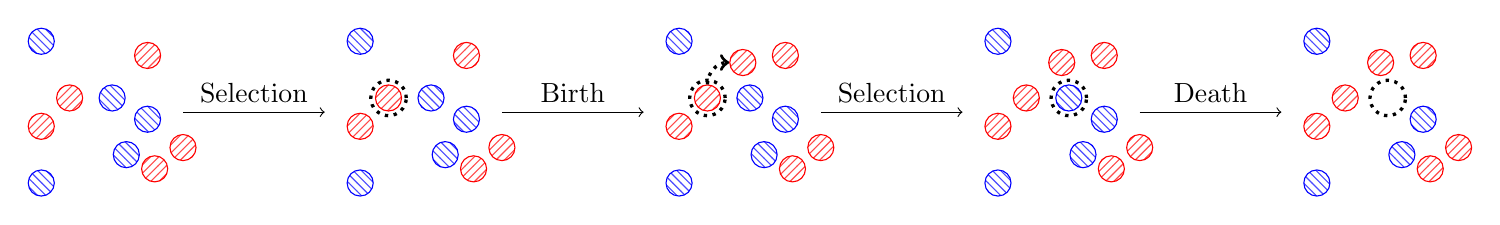
\begin{tikzpicture}[scale=.9]
	\node (A1) at (-1, -1) [circle, pattern=north west lines, pattern
        color=blue!70, draw=blue] {};
	\node (A2) at (-1, 1) [circle, pattern=north west lines, pattern
        color=blue!70, draw=blue] {};
	\node (A3) at (0, .2) [circle, pattern=north west lines, pattern
        color=blue!70, draw=blue] {};
	\node (A4) at (.2, -.6) [circle, pattern=north west lines, pattern
        color=blue!70, draw=blue] {};
	\node (A5) at (.5, -0.1) [circle, pattern=north west lines, pattern
        color=blue!70, draw=blue] {};
	\node (B1) at (-1, -.2) [circle, pattern=north east lines, pattern
        color=red!70, draw=red] {};
	\node (B2) at (1, -.5) [circle, pattern=north east lines, pattern
        color=red!70, draw=red] {};
	\node (B3) at (.5, .8) [circle, pattern=north east lines, pattern
        color=red!70, draw=red] {};
	\node (B4) at (-.6, .2) [circle, pattern=north east lines, pattern
        color=red!70, draw=red] {};
	\node (B5) at (.6, -.8) [circle, pattern=north east lines, pattern
        color=red!70, draw=red] {};

	\draw [->] (1, 0) -- (3, 0) node [above, pos=0.5] {Selection};

	\node (A1) at ($(A1) + (4.5, 0)$) [circle, pattern=north west lines,
        pattern color=blue!70, draw=blue] {};
	\node (A2) at ($(A2) + (4.5, 0)$) [circle, pattern=north west lines,
        pattern color=blue!70, draw=blue] {};
	\node (A3) at ($(A3) + (4.5, 0)$) [circle, pattern=north west lines,
        pattern color=blue!70, draw=blue] {};
	\node (A4) at ($(A4) + (4.5, 0)$) [circle, pattern=north west lines,
        pattern color=blue!70, draw=blue] {};
    \node (A5) at ($(A5) + (4.5, 0)$) [circle, pattern=north west lines,
        pattern color=blue!70, draw=blue] {};
	\node (B1) at ($(B1) + (4.5, 0)$) [circle, pattern=north east lines,
        pattern color=red!70, draw=red] {};
	\node (B2) at ($(B2) + (4.5, 0)$) [circle, pattern=north east lines,
        pattern color=red!70, draw=red] {};
	\node (B3) at ($(B3) + (4.5, 0)$) [circle, pattern=north east lines,
        pattern color=red!70, draw=red] {};
	\node (B4) at ($(B4) + (4.5, 0)$) [circle, pattern=north east lines,
        pattern color=red!70, draw=red] {};
	\node (B5) at ($(B5) + (4.5, 0)$) [circle, pattern=north east lines,
        pattern color=red!70, draw=red] {};

	\draw [dotted, very thick] (B4) circle (.25cm);

	\draw [->] (5.5, 0) -- (7.5, 0) node [above, pos=0.5] {Birth};

	\node (A1) at ($(A1) + (4.5, 0)$) [circle, pattern=north west lines,
        pattern color=blue!70, draw=blue] {};
	\node (A2) at ($(A2) + (4.5, 0)$) [circle, pattern=north west lines,
        pattern color=blue!70, draw=blue] {};
	\node (A3) at ($(A3) + (4.5, 0)$) [circle, pattern=north west lines,
        pattern color=blue!70, draw=blue] {};
	\node (A4) at ($(A4) + (4.5, 0)$) [circle, pattern=north west lines,
        pattern color=blue!70, draw=blue] {};
    \node (A5) at ($(A5) + (4.5, 0)$) [circle, pattern=north west lines,
        pattern color=blue!70, draw=blue] {};
	\node (B1) at ($(B1) + (4.5, 0)$) [circle, pattern=north east lines,
        pattern color=red!70, draw=red] {};
	\node (B2) at ($(B2) + (4.5, 0)$) [circle, pattern=north east lines,
        pattern color=red!70, draw=red] {};
	\node (B3) at ($(B3) + (4.5, 0)$) [circle, pattern=north east lines,
        pattern color=red!70, draw=red] {};
	\node (B4) at ($(B4) + (4.5, 0)$) [circle, pattern=north east lines,
        pattern color=red!70, draw=red] {};
	\node (B5) at ($(B5) + (4.5, 0)$) [circle, pattern=north east lines,
        pattern color=red!70, draw=red] {};

	\draw [dotted, very thick] (B4) circle (.25cm);
	\node (B6) at ($(B4) + (0.5, 0.5)$) [circle, pattern=north east lines,
        pattern color=red!70, draw=red] {};
	\draw [->, dotted, very thick] (B4) [out=90, in=180] to (B6);

	\draw [->] (10, 0) -- (12, 0) node [above, pos=0.5] {Selection};

	\node (A1) at ($(A1) + (4.5, 0)$) [circle, pattern=north west lines,
        pattern color=blue!70, draw=blue] {};
	\node (A2) at ($(A2) + (4.5, 0)$) [circle, pattern=north west lines,
        pattern color=blue!70, draw=blue] {};
	\node (A3) at ($(A3) + (4.5, 0)$) [circle, pattern=north west lines,
        pattern color=blue!70, draw=blue] {};
	\node (A4) at ($(A4) + (4.5, 0)$) [circle, pattern=north west lines,
        pattern color=blue!70, draw=blue] {};
    \node (A5) at ($(A5) + (4.5, 0)$) [circle, pattern=north west lines,
        pattern color=blue!70, draw=blue] {};
	\node (B1) at ($(B1) + (4.5, 0)$) [circle, pattern=north east lines,
        pattern color=red!70, draw=red] {};
	\node (B2) at ($(B2) + (4.5, 0)$) [circle, pattern=north east lines,
        pattern color=red!70, draw=red] {};
	\node (B3) at ($(B3) + (4.5, 0)$) [circle, pattern=north east lines,
        pattern color=red!70, draw=red] {};
	\node (B4) at ($(B4) + (4.5, 0)$) [circle, pattern=north east lines,
        pattern color=red!70, draw=red] {};
	\node (B5) at ($(B5) + (4.5, 0)$) [circle, pattern=north east lines,
        pattern color=red!70, draw=red] {};
	\node (B6) at ($(B6) + (4.5, 0)$) [circle, pattern=north east lines,
        pattern color=red!70, draw=red] {};

	\draw [dotted, very thick] (A3) circle (.25cm);

	\draw [->] (14.5, 0) -- (16.5, 0) node [above, pos=0.5] {Death};

	\node (A1) at ($(A1) + (4.5, 0)$) [circle, pattern=north west lines,
        pattern color=blue!70, draw=blue] {};
	\node (A2) at ($(A2) + (4.5, 0)$) [circle, pattern=north west lines,
        pattern color=blue!70, draw=blue] {};
	\node (A3) at ($(A3) + (4.5, 0)$) {};
	\node (A4) at ($(A4) + (4.5, 0)$) [circle, pattern=north west lines,
        pattern color=blue!70, draw=blue] {};
    \node (A5) at ($(A5) + (4.5, 0)$) [circle, pattern=north west lines,
        pattern color=blue!70, draw=blue] {};
	\node (B1) at ($(B1) + (4.5, 0)$) [circle, pattern=north east lines,
        pattern color=red!70, draw=red] {};
	\node (B2) at ($(B2) + (4.5, 0)$) [circle, pattern=north east lines,
        pattern color=red!70, draw=red] {};
	\node (B3) at ($(B3) + (4.5, 0)$) [circle, pattern=north east lines,
        pattern color=red!70, draw=red] {};
	\node (B4) at ($(B4) + (4.5, 0)$) [circle, pattern=north east lines,
        pattern color=red!70, draw=red] {};
	\node (B5) at ($(B5) + (4.5, 0)$) [circle, pattern=north east lines,
        pattern color=red!70, draw=red] {};
	\node (B6) at ($(B6) + (4.5, 0)$) [circle, pattern=north east lines,
        pattern color=red!70, draw=red] {};

	\draw [dotted, very thick] (A3) circle (.25cm);
\end{tikzpicture}
\end{document}

    \caption{A diagrammatic representation of a Moran process}
    \label{fig:moran_process}
\end{figure}

The Moran process was initially introduced in \cite{Moran1957}. It has since
been used in a variety of settings including the understanding of the spread of
cooperative and non-cooperative behaviour such as cancer \cite{West2016} and the
emergence of cooperative behaviour in spatial topologies \cite{Nowak2017}.
However these works mainly consider non-sophisticated strategies. Some work has
looked at evolutionary stability of strategies within the Prisoner's Dilemma
\cite{Li2014} but this is not done in the more widely-used setting of the Moran
process, rather in terms of infinite population stability. In \cite{Baek2016}
Moran processes are studied in a theoretical framework for a small subset of
strategies.  The subset included memory one strategies, strategies that recall
the events of the previous round only.

Of particular interest are the zero determinant strategies introduced in
\cite{Press2012} and highly-praised \cite{Stewart2012} it was argued that
generous ZD strategies are robust against invading strategies. However, in
\cite{Lee2015} a strategy using machine learning techniques was capable of
resisting invasion and also able to invade any memory one strategy.  Recent work
\cite{Hilbe2017} has investigated the effect of memory length on strategy
performance and the emergence of cooperation but this is not done in Moran
process context and only considers specific cases of memory 2 strategies.  In
\cite{Adami2013} it was recognized that many zero determinant strategies do not
fare well against themselves. This is a disadvantage for the Moran process where
the best strategies cooperate well with other players using the same strategy.

The contribution of this work is a detailed and extensive analysis of absorption
probabilities for 164 strategies. These strategies and the numerical simulations
are from~\cite{axelrodproject} which is an open source research library written
for the study of the IPD\@. The strategies and simulation frameworks are
automatically tested to an extraordinarily high degree of coverage in accordance
with best research software practices. The large
number of strategies are available thanks to the open source nature of the
project with over 40 contributions made by different programmers and researchers.

Section~\ref{sec:methodology} will explain the methodological approach used,
Section~\ref{sec:validation} will validate the methodology by comparing
simulated results to analytical results in some cases. The main results of this
manuscript are presented in Section~\ref{sec:empirical_results} which will
present a detailed analysis of all the data generated. Finally,
Section~\ref{sec:conclusion} will conclude and offer future avenues for the work
presented here.

\section{Methodology}\label{sec:methodology}

To carry out this large numerical experiment, 164 strategies are used from the
axelrod library: \cite{axelrodproject}.

The axelrod library contains many machine learning based strategies trained
with reinforcement learning algorithms. This work includes three additional
strategies trained specifically to excel at the Moran process.
Appendix~\ref{app:list_of_players} shows all the players in question. More
information about each player can be obtained in the documentation for
\cite{axelrodproject}. There are 43stochastic and
124deterministic strategies. Their memory
depth, defined by the number of rounds of history used by the strategy each round,
is shown in Table~\ref{tbl:memory_depth_count}. The memory depth is infinite if
the strategy uses the entire history of play (whatever its length). For example,
a strategy that utilizes a handshaking mechanism where the opponents actions
on the first few rounds of play determines the strategies subsequent behavior
would have infinite memory depth.

All of the
strategies are trained with an evolutionary algorithm that perturbs strategy
% TODO Add a generic text book reference
parameters and optimizes an objective function, such as the mean total score
against all other opponents or the mean fixation probability over a large
number of Moran processes. The objective functions can include standard
variations such as noisy matches, varying the number of rounds of play, and the
other typical parameters used for the IPD. Variation is introduced via mutation
and crossover of parameters, and the best performing strategies are carried to
the next generation along with new variants. Similar methods appear in the
literature \cite{Ashlock2006}.

All of our training code is available in the
Axelrod repository with documentation to train new strategies easily. Training
% TODO Include link etc
typically takes less than 200 iterations and can be completed within several
hours on commodity hardware.  The three strategies trained specifically for
this study are Trained FSM 1, 2, and 3 (TF1 - TF3), based on finite state
machines of 16, 16, and 8 states respectively (see Figures \ref{}).
% TODO Include images of FSMs
These strategies were trained with the objective function of mean fixation
probabilities for Moran processes starting at initial population states
consisting of \(N/2\) individuals of the training candidates and \(N/2\)
individuals of an opponent strategy, for all of the short run time strategies
in the library (approximately 150 opponents at the time of training):

\begin{itemize}
	\item TF1 \(N=12\), 0\% noise, 10000 repetitions per match
	\item TF2 \(N=10\), 0\% noise, 10000 repetitions per match
	\item TF3 \(N=8\), 1\% noise, 100 repetitions per match
\end{itemize}

Each matchup of players was run to fixation for the specified number of
repetitions to estimate the absorption probabilities. The trained algorithms
were run for less than 50 generations.

TF1 has an initial handshake of CCD and cooperates if the opponent matches.
However if the opponent later defects, TF1 will respond in kind, so the
handshake is not permanent. Only one player (Prober 4 \cite{prison}) manages to
achieve cooperation with TF1 after about 20 rounds of play.

TF2 always starts
with CD and will defect against opponents that start with DD. It plays CDD
against itself and then cooperates thereafter. There is a longer complex
handshake which eventually results in mutual cooperation with Firm but Fair,
Fortress3, Fortress4, and Grofman (always) and Evolved HMM 5 and GTFT
(depending on the random seed).

TF3 cooperates and defects with
various cycles depending on the opponent's actions. TF3 will mutually
cooperate with any strategy and only tolerates a few defections before
defecting for the rest of match. It is similar to but not exactly the same as
Fool Me Once, a strategy that cooperates until the opponent has defected twice
(not necessarily consecutively), and defects indefinitely thereafter. Though a
product of training with a Moran objective, it was selected for inclusion
because of the lack of an apparent handshake.

For both TF1 and TF2 a handshake
mechanism naturally emerges from the structure of the underlying finite state
machine. This behavior is an outcome of the evolutionary process and is in no
way hard-coded or included via an additional mechanism. Some of the existing
strategies in the library were trained on earlier versions of the library
(smaller total opponents used in training) based on neural networks, lookup
tables and stochastic variants trained with a particle swarm algorithm, finite
state machines and a stochastic variant mimicking hidden Markov models, and
neural networks. These strategies were trained to win IPD tournaments using an
objective function that computes the mean match payoffs against a collection of
opponents. Detailed descriptions and the performance of these strategies in IPD
tournaments will be described in another manuscript.
% TODO Think of how to reference this upcoming manuscript
% TODO Move the section below to the discussion for particular
% cases and/or conclusion
These strategies trained with the mean score
objective are among the best invaders in the library but are not as resistant
to invasion as the strategies trained using a Moran objective function (see
Tables \ref{}). These strategies include trained finite state machine
strategies, but they do not appear to have handshaking mechanisms. Therefore it
is reasonable to conclude that the objective function is the cause of the
emergence of handshaking mechanisms.
The payoff maximizing strategies
typically will not defect before the opponent's first defection, possibly
because the training strategy collection contains a significant portion of
strategies such as Grudger and Fool Me Once that retaliate harshly by defecting
for the remainder of the match if the opponent has more than a small number of
cumulative defections. Paradoxically it is necessary to defect in order to
achieve mutual cooperation with opponents using the same strategy but not with
other opponents. A handshake requires at least one defection and there is
selective pressure to defect as few times as possible to achieve the
self-recognition mechanism. It is also unwise to defect on the first move as
some strategies additionally retaliate first round defections. So the
handshakes used by TF1 and TF2, and CS, are in some sense optimal.  These
discoveries may have significant ramifications regarding the evolution of
cooperation and forgiveness in biological organisms and social interactions
between humans.

\begin{table}[!hbtp]
    \centering
        \begin{tabular}{lrrrrrrrrrrrrrrrr}
\toprule
Memory Depth &   0   &   1   &   2   &   3   &   4   &   5   &   6   &   9   &   10  &   11  &   12  &   16  &   20  &   40  &   200 &  \(\infty\)   \\
\midrule
Count &     3 &    34 &    12 &     8 &     2 &     6 &     1 &     1 &     5 &     1 &     1 &     2 &     2 &     2 &     1 &    86 \\
\bottomrule
\end{tabular}

        \caption{Memory depth}
        \label{tbl:memory_depth_count}
\end{table}

Each strategy pair is run for 1000 runs of the Moran process to fixation
with starting population distributions of $(1, N-1)$,
$(N/2, N/2)$ and $(N-1 , 1)$, for \(N\) from 2 through 14. The
% TODO Change 14 to 12 if we do not use the 14 case.
fixation probability is then empirically computed for each combination of
starting distribution and value of \(N\).

Our software can carry out exact simulations of the Moran process. Since some of
the strategies have a high computational cost or are stochastic, we sample
from a large number of match outcomes for the pairs of players for use in computing
fitnesses in the Moran process. This approach was verified to agree with unsampled
calculations to a high degree of accuracy in specific cases.
% TODO Perhaps write some pseudo code for this?

Figure~\ref{fig:number_of_stochastic_match_outcomes} shows the distribution of
the number of outcomes between all strategy pairs.
% TODO is this true? the distribution also matters, not just the number of outcomes
% TODO Good point, we could (if we wanted to) go down the line of checking
% specific distributions etc or perhaps we just remove and point at the good
% fits in the Validation section as a justification.


\begin{figure}[!hbtp]
    \centering
    \begin{subfigure}[t]{.5\textwidth}
        \centering
        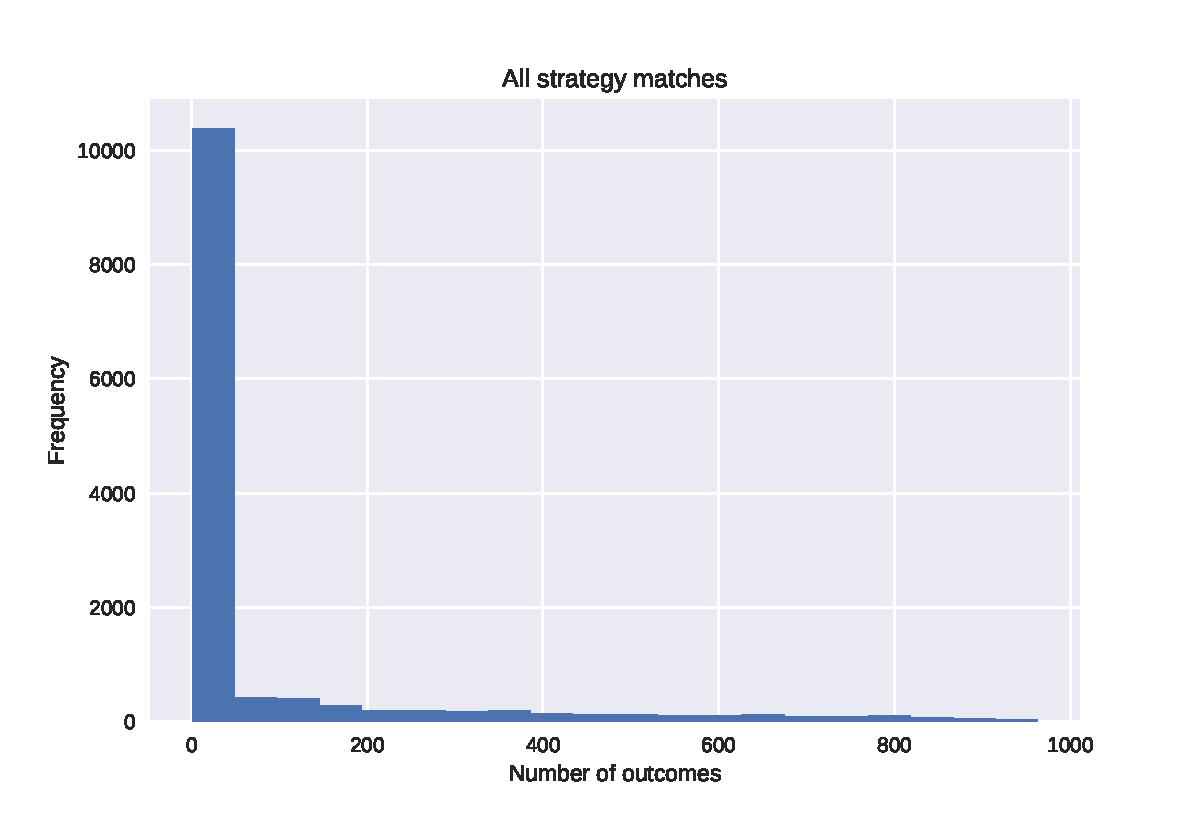
\includegraphics[width=.9\textwidth]{./img/number_of_match_outcomes.pdf}
        \caption{All matches}
    \end{subfigure}%
    ~
    \begin{subfigure}[t]{.5\textwidth}
        \centering
        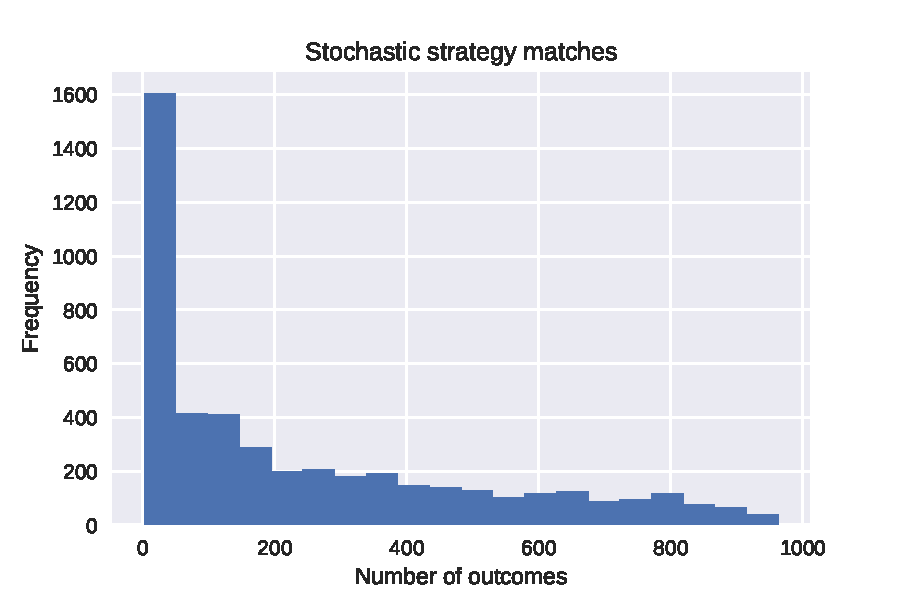
\includegraphics[width=.9\textwidth]{./img/number_of_stochastic_match_outcomes.pdf}
        \caption{Stochastic matches}
    \end{subfigure}%
    \caption{The distribution of the number of unique outcomes used as the
    cached results}
    \label{fig:number_of_stochastic_match_outcomes}
\end{figure}

Section~\ref{sec:validation} will validate the methodology used here against
known theoretic results.

\section{Validation}\label{sec:validation}

As described in \cite{Nowak} consider the payoff matrix:

\begin{equation}\label{equ:payoff_matrix}
    M = \begin{pmatrix}
        a, b\\
        c, d
        \end{pmatrix}
\end{equation}

The expected payoffs of \(i\) players of the first type in a population with \(N
- i\) players of the second type are given by:

\begin{equation}\label{equ:expected_payoff_one}
    F_i = \frac{a(i - 1) + b(N - i)}{N - 1}
\end{equation}

\begin{equation}\label{equ:expected_payoff_two}
    G_i = \frac{ci + d(N - i - 1)}{N - 1}
\end{equation}

With an intensity of selection \(\omega\) the fitness of both strategies is
given by:

\begin{equation}\label{equ:expected_payoff_one}
    f_i = 1 - \omega + \omega F_i
\end{equation}

\begin{equation}\label{equ:expected_payoff_two}
    g_i = 1 - \omega + \omega G_i
\end{equation}

The transitions within the birth death process that underpins the Moran process
are then given by:

\begin{align}
    p_{i, i+1}&= \frac{if_i}{if_i+(N-i)g_i}\frac{N-i}{N}\label{equ:p_up}\\
    p_{i, i-1}&= \frac{(N-i)g_i}{if_i+(N-i)g_i}\frac{i}{N}\label{equ:p_down}\\
    p_{ii} &= 1 - p_{i, i+1} - p_{i, i-1}\label{equ:p_stay}
\end{align}

Using this it is a known result that the fixation probability of the first
strategy in a population of \(i\) individuals of the first type (and \(N-i\)
individuals of the second. We have:

\begin{equation}\label{equ:fixation_probability}
x_i = \frac{1 + \sum_{j=1}^{i-1}\prod_{k=1}^{j}\gamma_j}{1 + \sum_{j=1}^{N-1}
      \prod_{k=1}^{j}\gamma_j}
\end{equation}

where:

\[
\gamma_j = \frac{p_{j, j-1}}{p_{j, j+1}}
\]

A neutral strategy will have fixation probability $x_i = i/N$. Alternatively,
we can frame the outcomes in terms of relative fitness. For a strategy
of relative fitness $r$ the fixation probability is well-known to be

\[ x_i = \frac{1 - r^{-i}}{1 - r^{-N}} \]

We can use this formula to compute a value $r_i$ that produces the observed
value $x_i$, noting that for arbitrary strategies the value of this
effective relative fitness is dependent on $i$ and $N$.

Comparisons of \(x_1, x_{N/2}, x_{N-1}\) are shown in
Figure~\ref{fig:comparison_deterministic}. The points represent the simulated
values and the line shows the theoretical value. Note that these are all
deterministic strategies and show a perfect match up between the expected value
of (\ref{equ:fixation_probability}) and the actual Moran process for all
strategies pairs.

\begin{figure}[!hbtp]
    \centering
    \begin{subfigure}[t]{.3\textwidth}
        \centering
        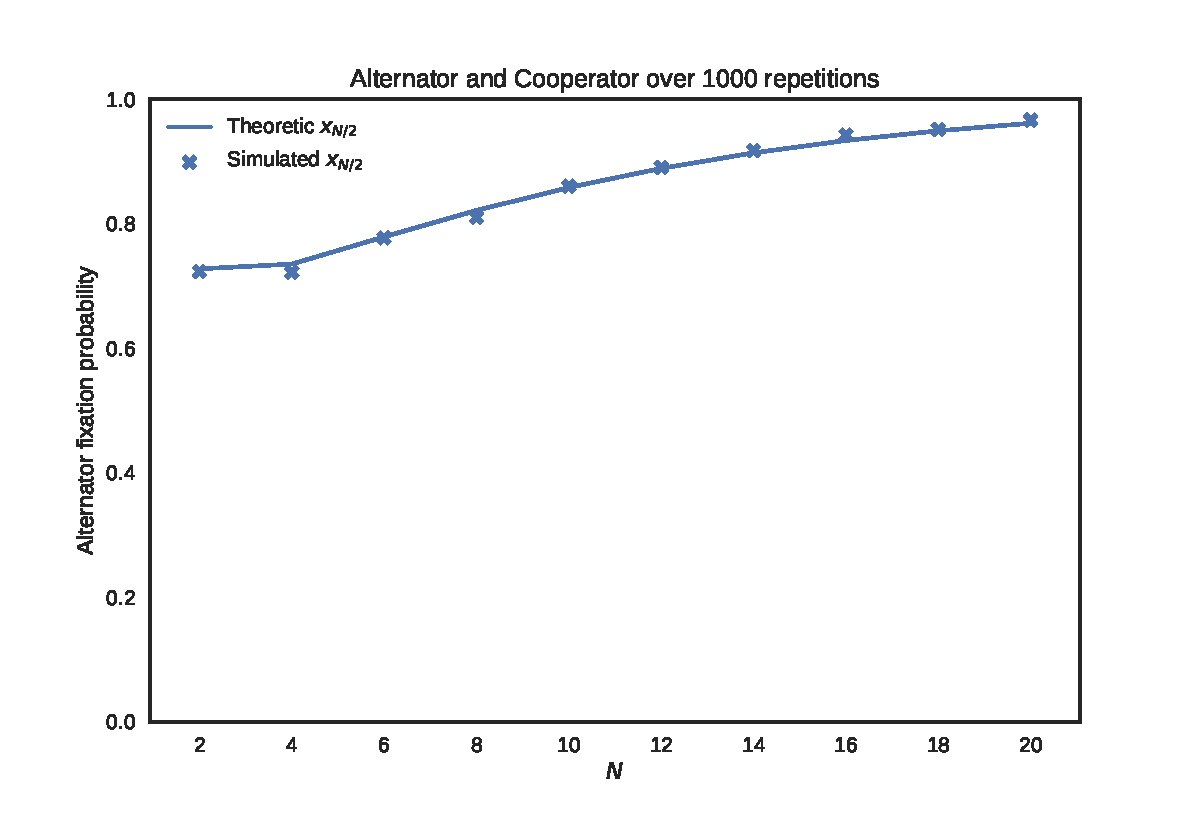
\includegraphics[width=.8\textwidth]{./img/Alternator_v_Cooperator.pdf}
        \caption{Alternator and Cooperator}
    \end{subfigure}%
    ~
    \begin{subfigure}[t]{.3\textwidth}
        \centering
        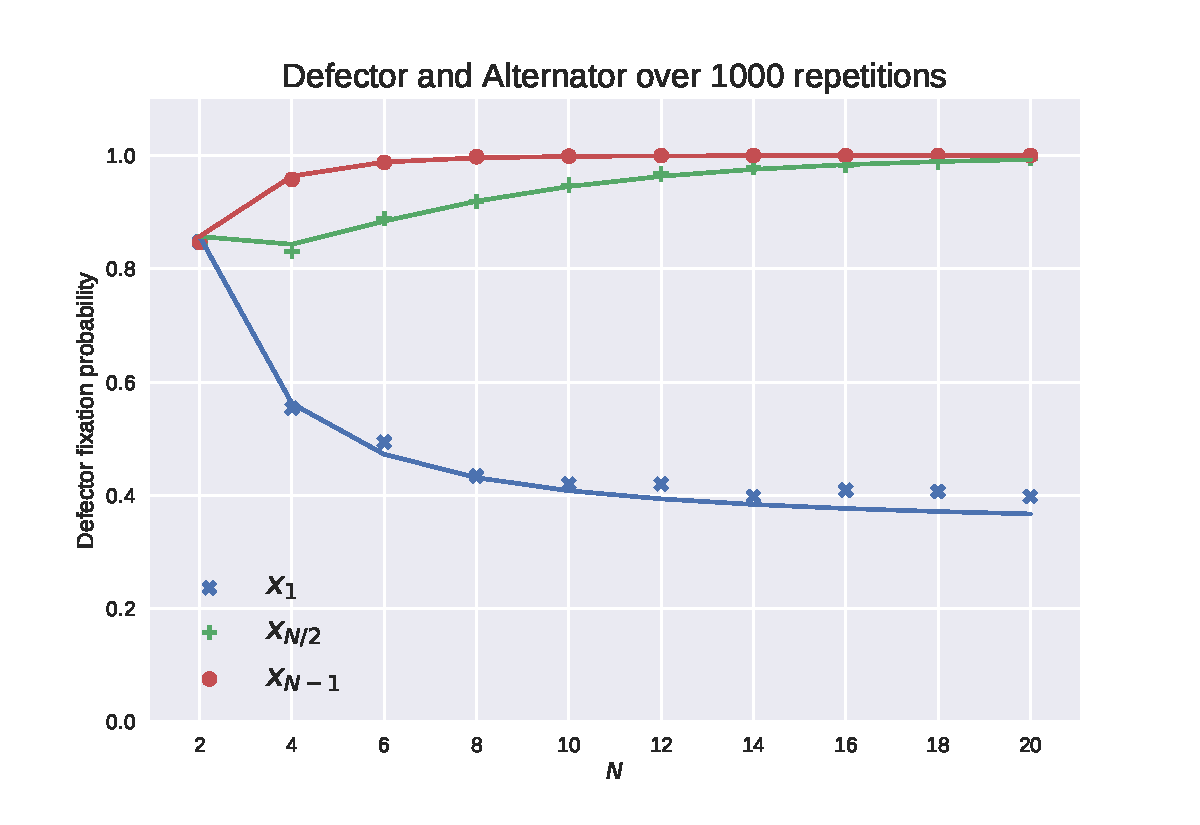
\includegraphics[width=.8\textwidth]{./img/Defector_v_Alternator.pdf}
        \caption{Defector and Alternator}
    \end{subfigure}%
    ~
    \begin{subfigure}[t]{.3\textwidth}
        \centering
        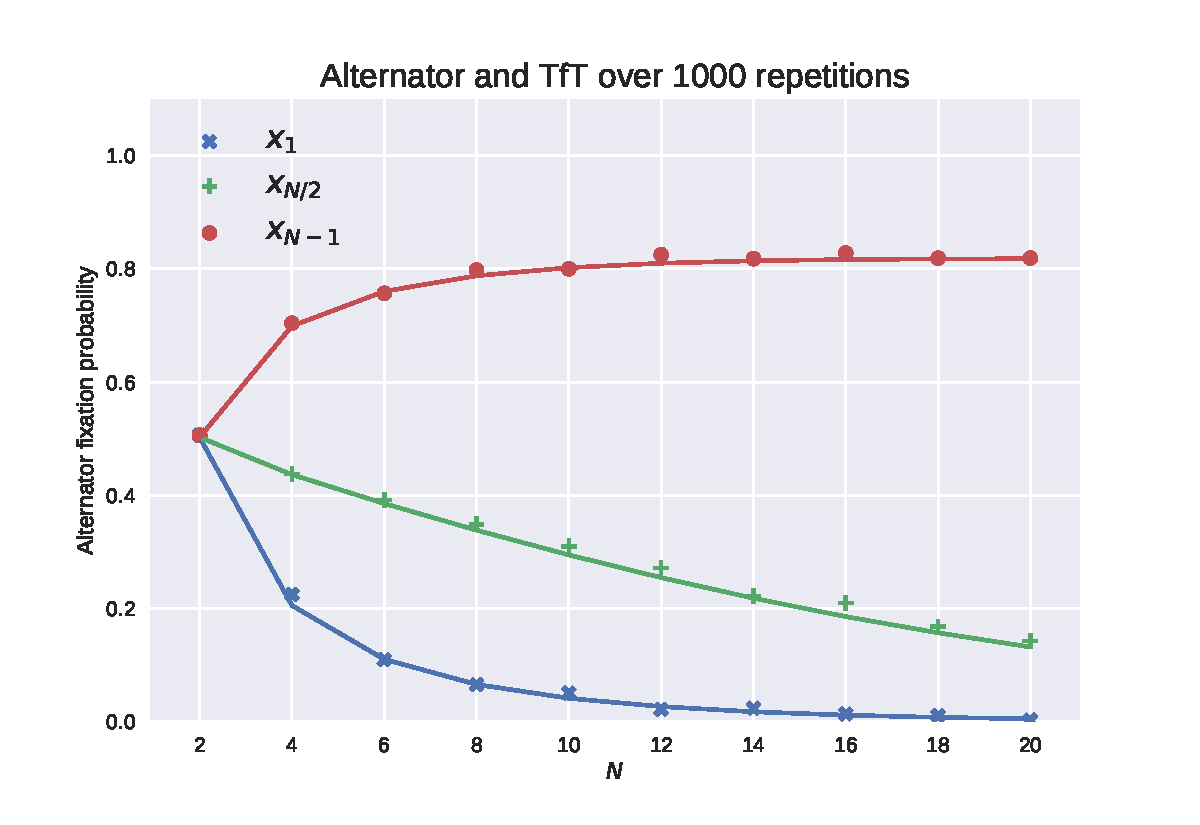
\includegraphics[width=.8\textwidth]{./img/Alternator_v_TfT.pdf}
        \caption{Alternator and Tit For Tat}
    \end{subfigure}%

    \begin{subfigure}[t]{.3\textwidth}
        \centering
        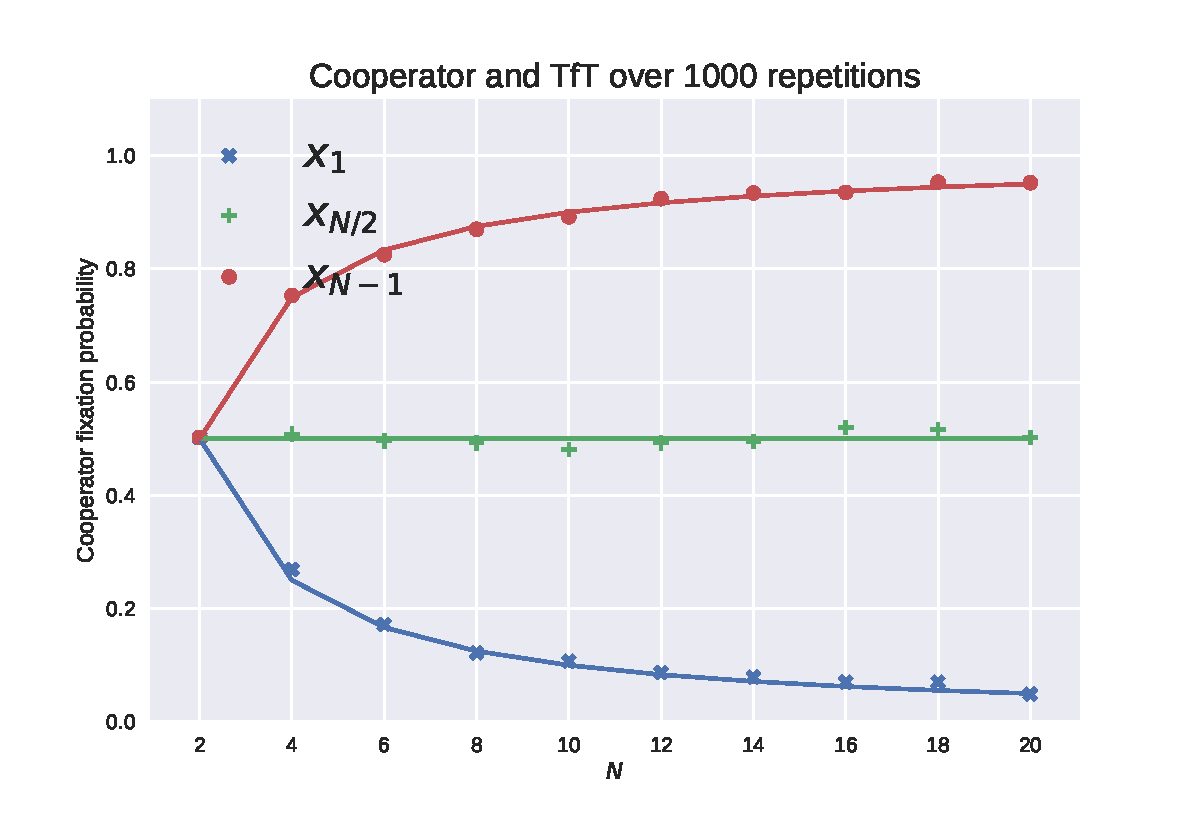
\includegraphics[width=.8\textwidth]{./img/Cooperator_v_TfT.pdf}
        \caption{Cooperator and Tit For Tat}
    \end{subfigure}%
    ~
    \begin{subfigure}[t]{.3\textwidth}
        \centering
        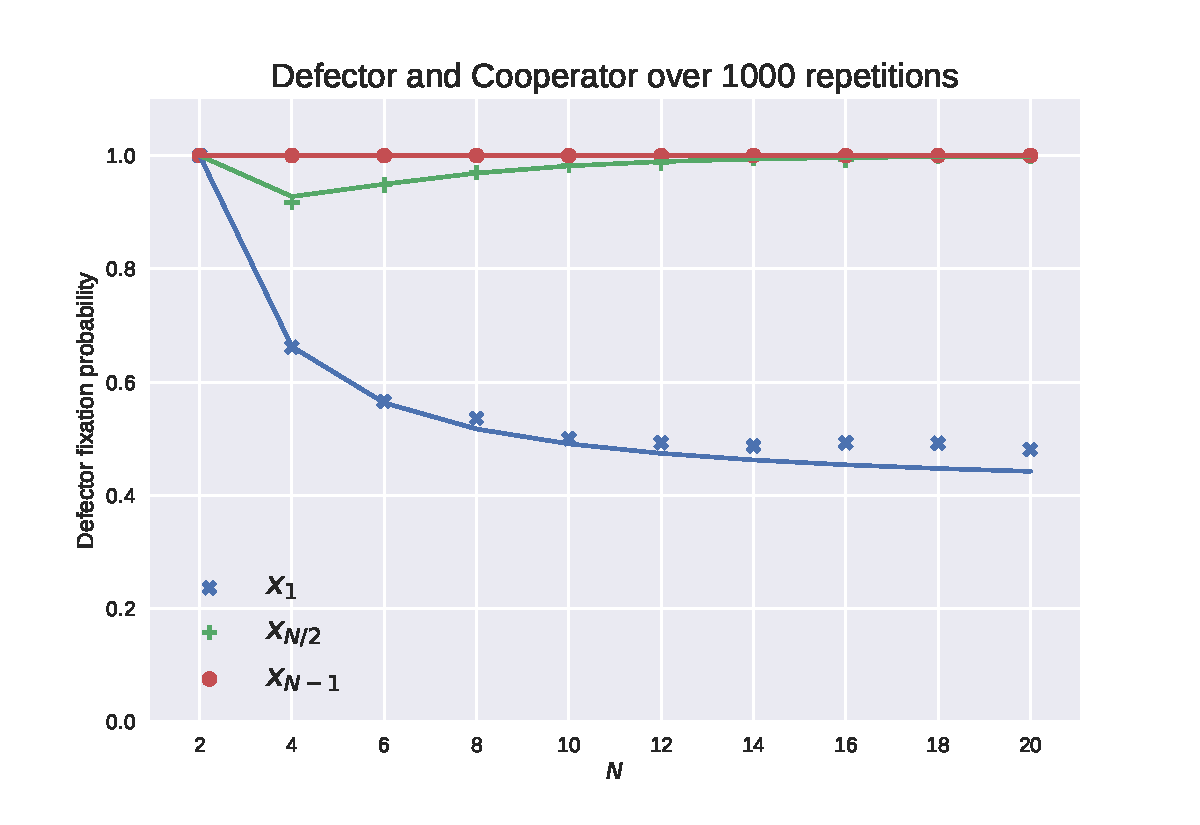
\includegraphics[width=.8\textwidth]{./img/Defector_v_Cooperator.pdf}
        \caption{Defector and Cooperator}
    \end{subfigure}%
    ~
    \begin{subfigure}[t]{.3\textwidth}
        \centering
        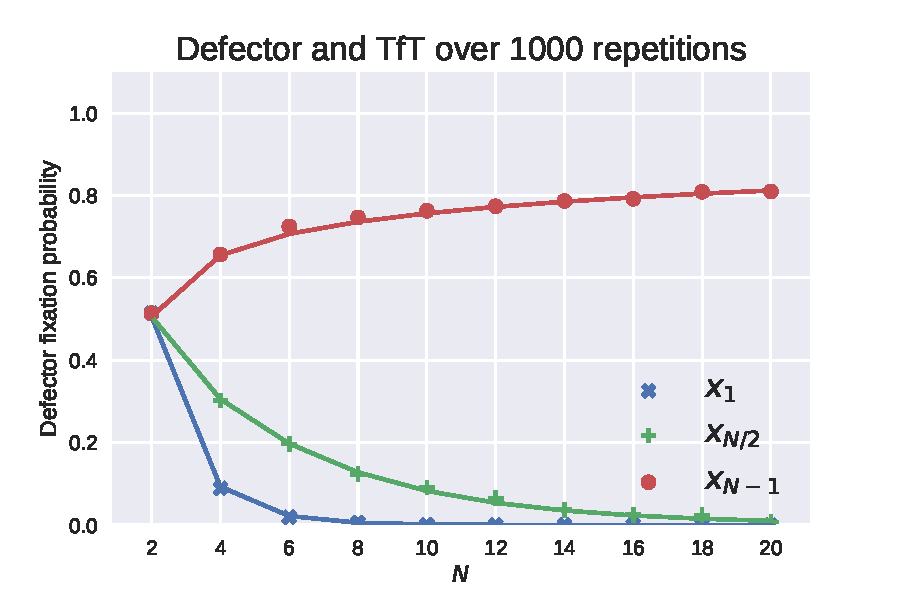
\includegraphics[width=.8\textwidth]{./img/Defector_v_TfT.pdf}
        \caption{Defector and Tit For Tat}
    \end{subfigure}%

    \begin{subfigure}[t]{.3\textwidth}
        \centering
        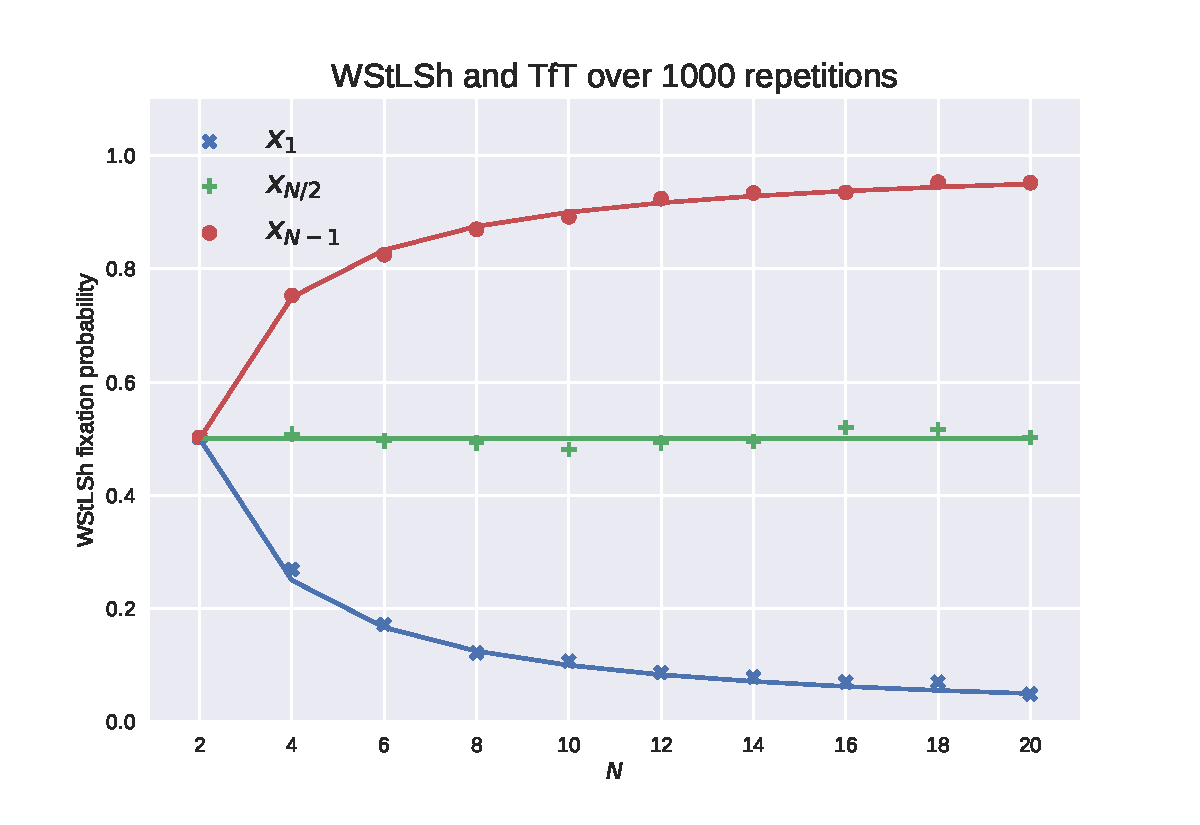
\includegraphics[width=.8\textwidth]{./img/WStLSh_v_TfT.pdf}
        \caption{Win Stay Lose Shift and Tit For Tat}
    \end{subfigure}%
    ~
    \begin{subfigure}[t]{.3\textwidth}
        \centering
        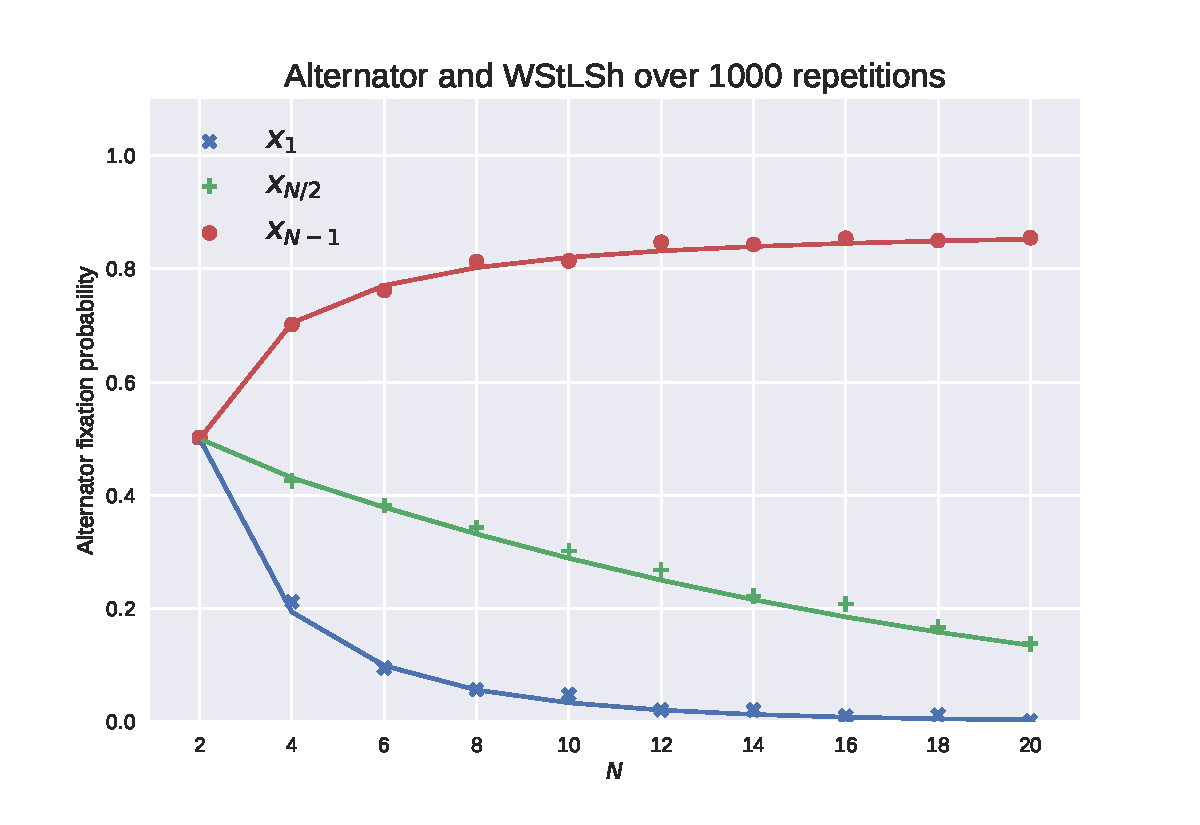
\includegraphics[width=.8\textwidth]{./img/Alternator_v_WStLSh.pdf}
        \caption{Alternator and Win Stay Lose Shift}
    \end{subfigure}%
    ~
    \begin{subfigure}[t]{.3\textwidth}
        \centering
        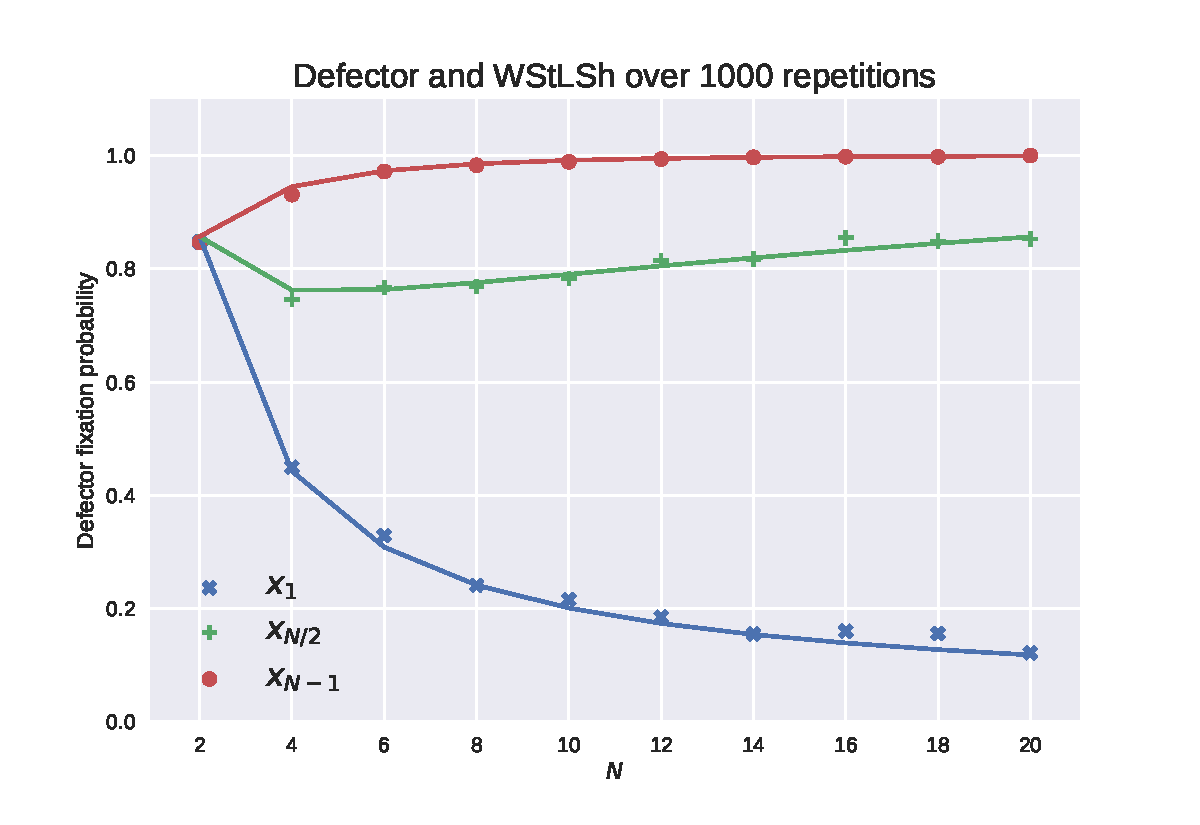
\includegraphics[width=.8\textwidth]{./img/Defector_v_WStLSh.pdf}
        \caption{Defector and Win Stay Lose Shift}
    \end{subfigure}%
    \caption{Comparison of theoretic and actual Moran Process fixation
             probabilities for \textbf{deterministic} strategies}
    \label{fig:comparison_deterministic}
\end{figure}

\begin{figure}[!hbtp]
    \centering
    \begin{subfigure}[t]{.3\textwidth}
        \centering
        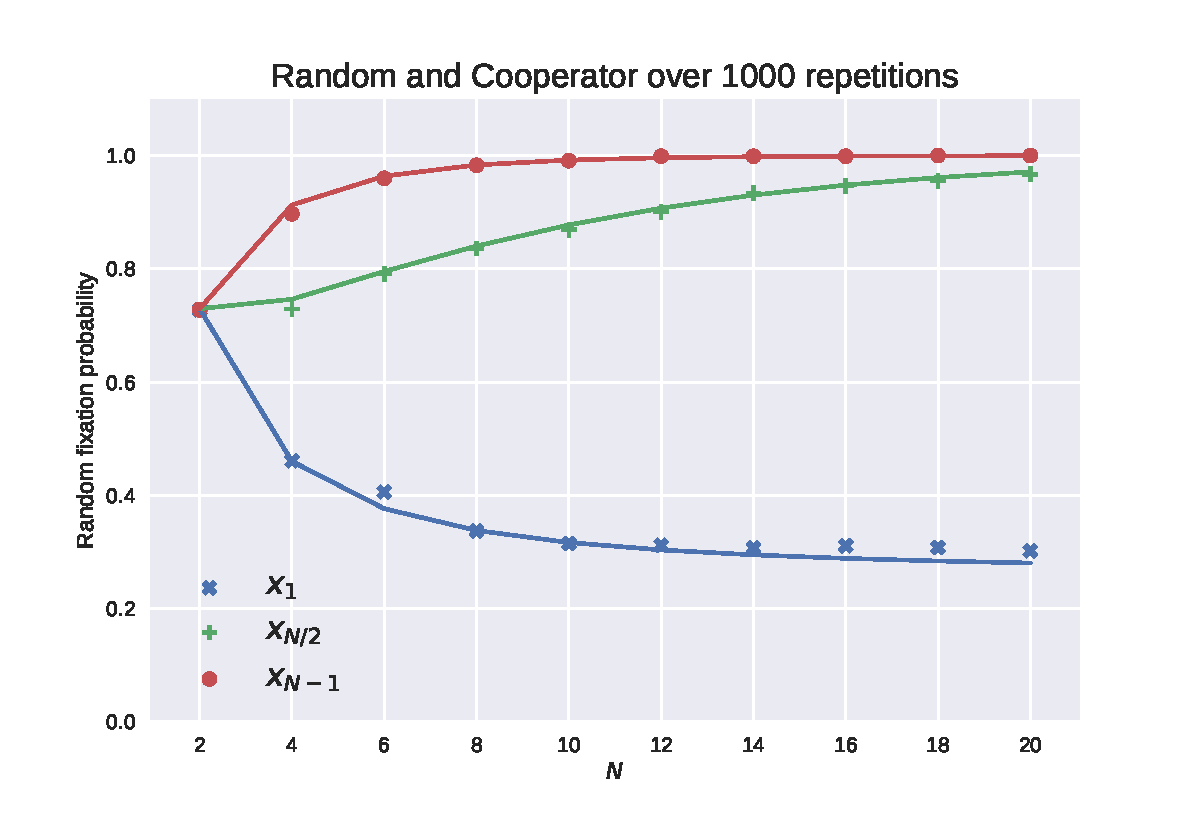
\includegraphics[width=.8\textwidth]{./img/Random_v_Cooperator.pdf}
        \caption{Random and Cooperator}
    \end{subfigure}%
    ~
    \begin{subfigure}[t]{.3\textwidth}
        \centering
        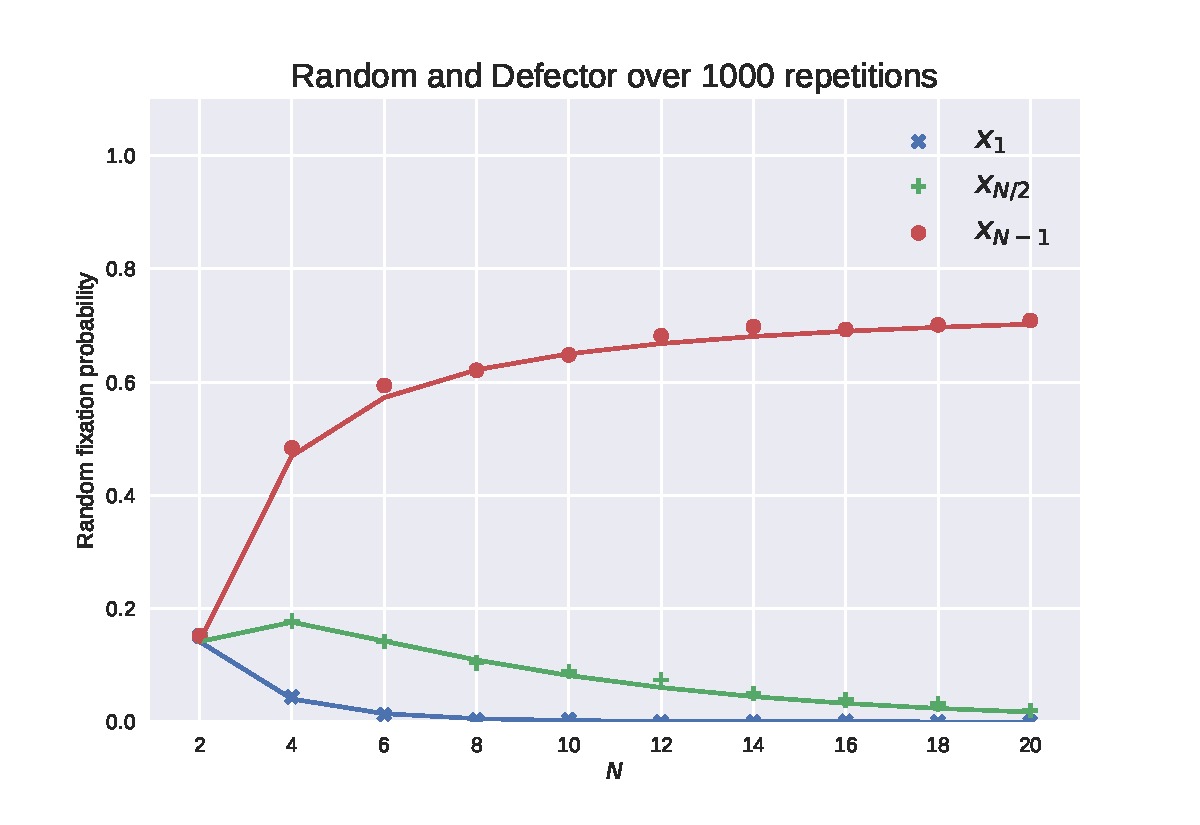
\includegraphics[width=.8\textwidth]{./img/Random_v_Defector.pdf}
        \caption{Random and Defector}
    \end{subfigure}%
    ~
    \begin{subfigure}[t]{.3\textwidth}
        \centering
        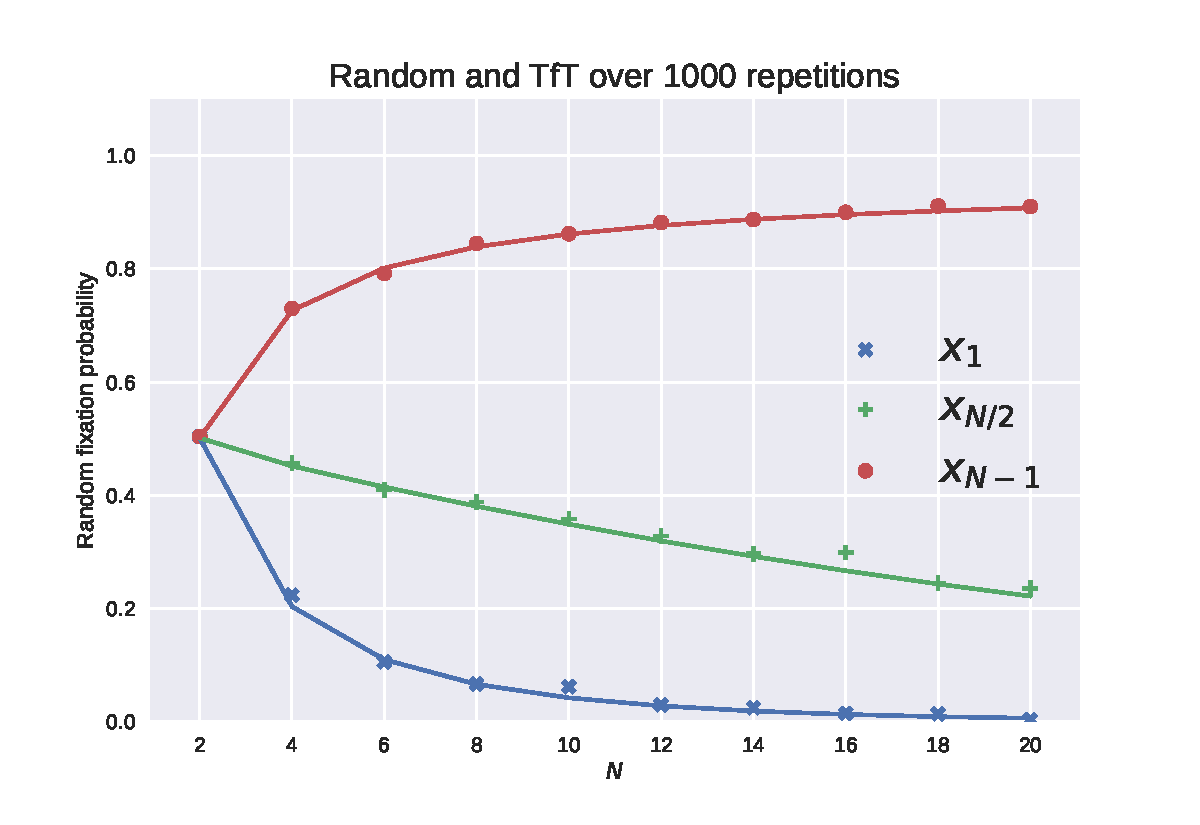
\includegraphics[width=.8\textwidth]{./img/Random_v_TfT.pdf}
        \caption{Random and Tit For Tat}
    \end{subfigure}%

    \begin{subfigure}[t]{.3\textwidth}
        \centering
        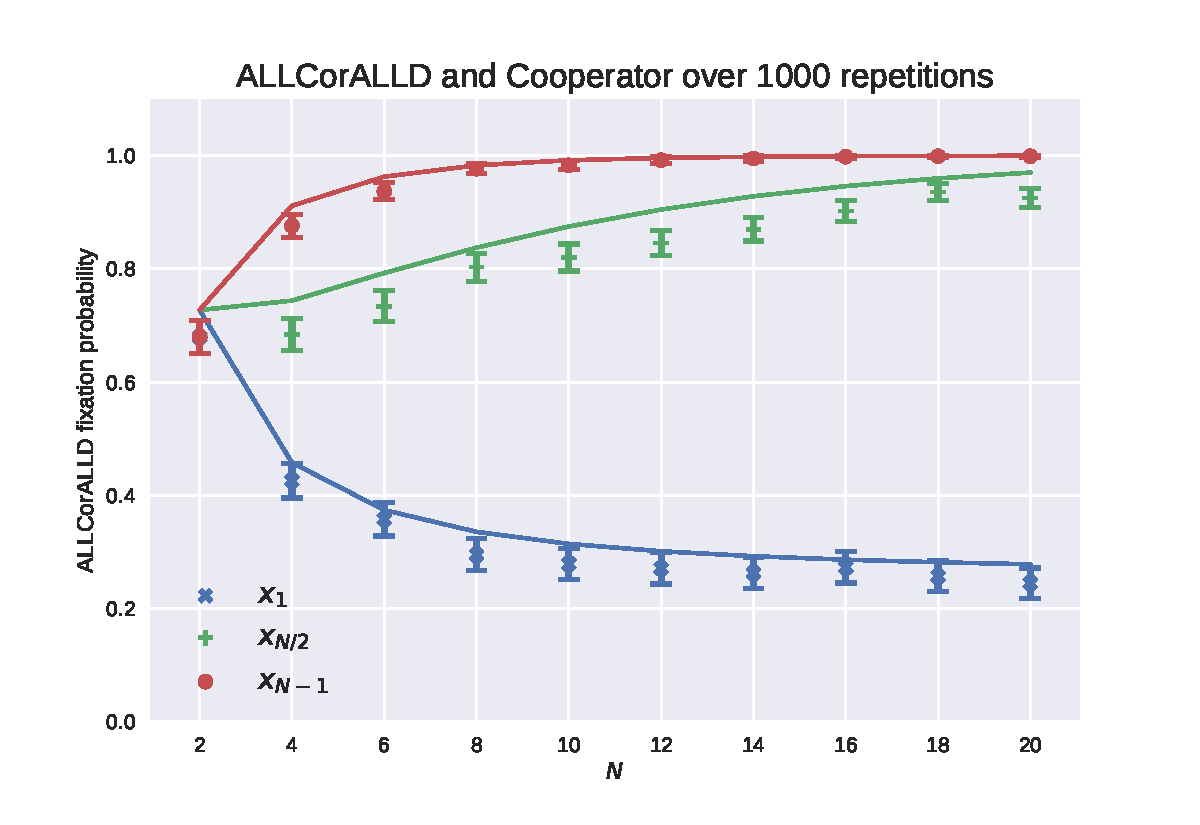
\includegraphics[width=.8\textwidth]{./img/ALLCorALLD_v_Cooperator.pdf}
        \caption{All C or all D and Cooperator}
    \end{subfigure}%
    ~
    \begin{subfigure}[t]{.3\textwidth}
        \centering
        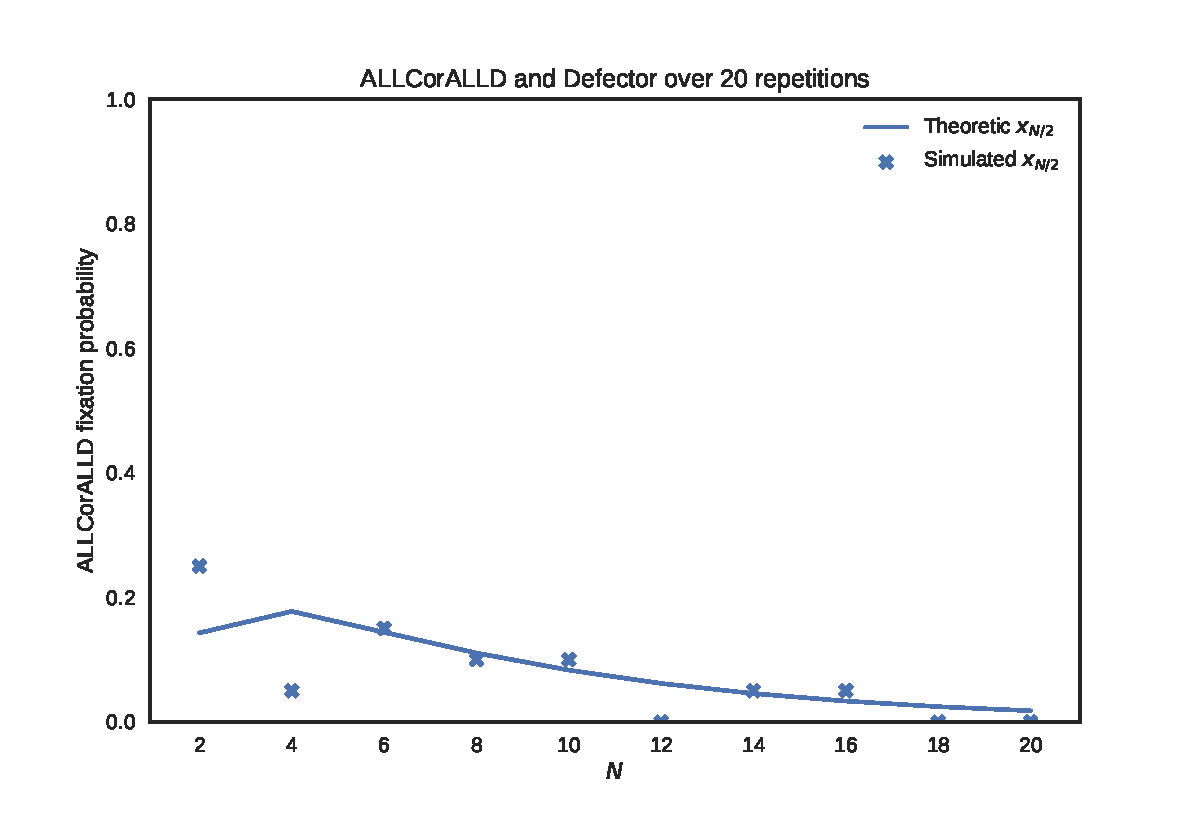
\includegraphics[width=.8\textwidth]{./img/ALLCorALLD_v_Defector.pdf}
        \caption{All C or all D and Defector}
    \end{subfigure}%
    ~
    \begin{subfigure}[t]{.3\textwidth}
        \centering
        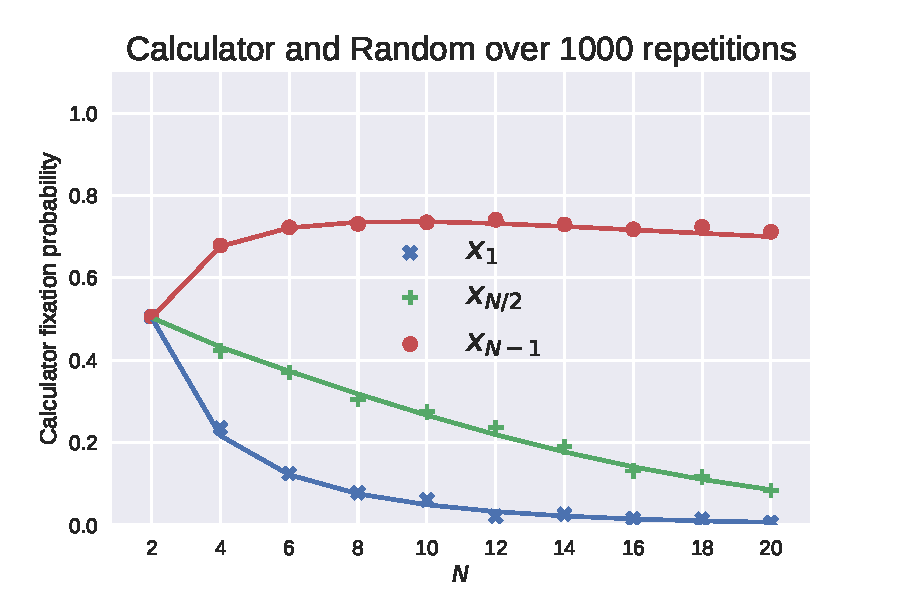
\includegraphics[width=.8\textwidth]{./img/Calculator_v_Random.pdf}
        \caption{Calculator and Random}
    \end{subfigure}%

    \begin{subfigure}[t]{.3\textwidth}
        \centering
        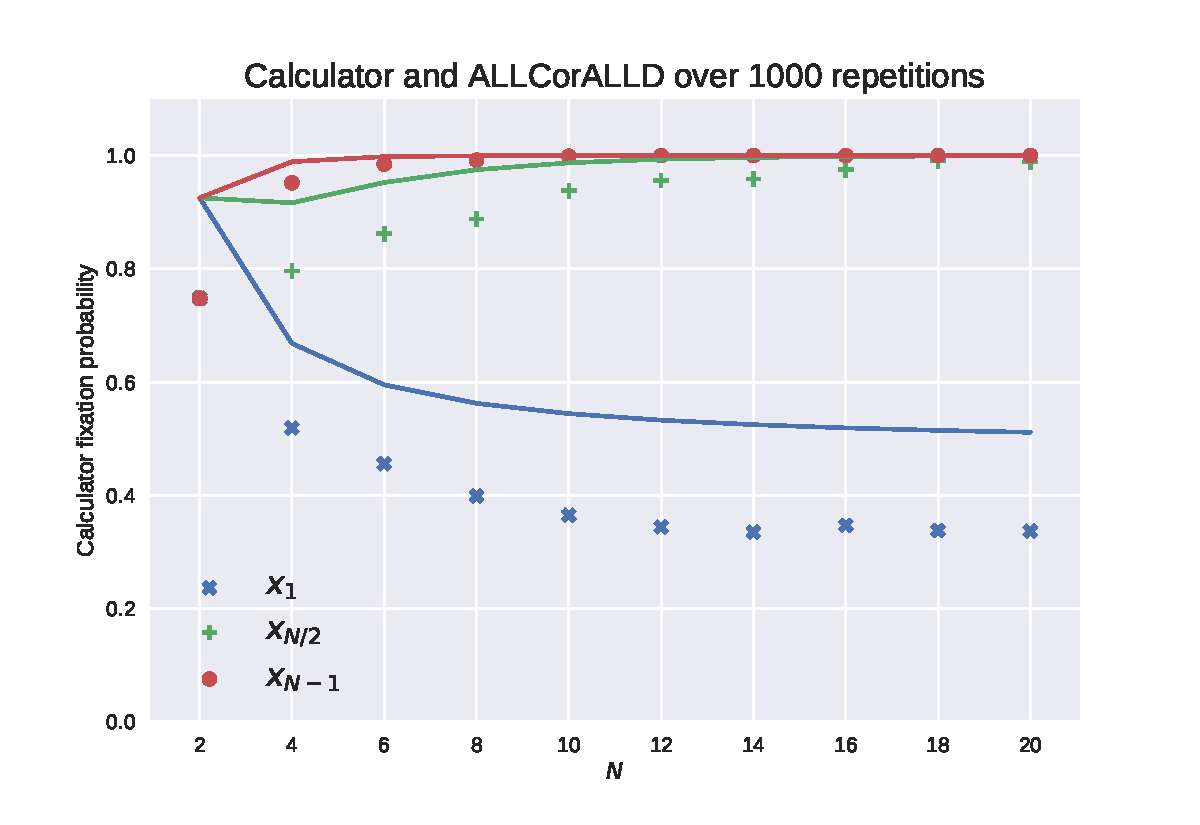
\includegraphics[width=.8\textwidth]{./img/Calculator_v_ALLCorALLD.pdf}
        \caption{Calculator and All C or all D}
    \end{subfigure}%
    ~
    \begin{subfigure}[t]{.3\textwidth}
        \centering
        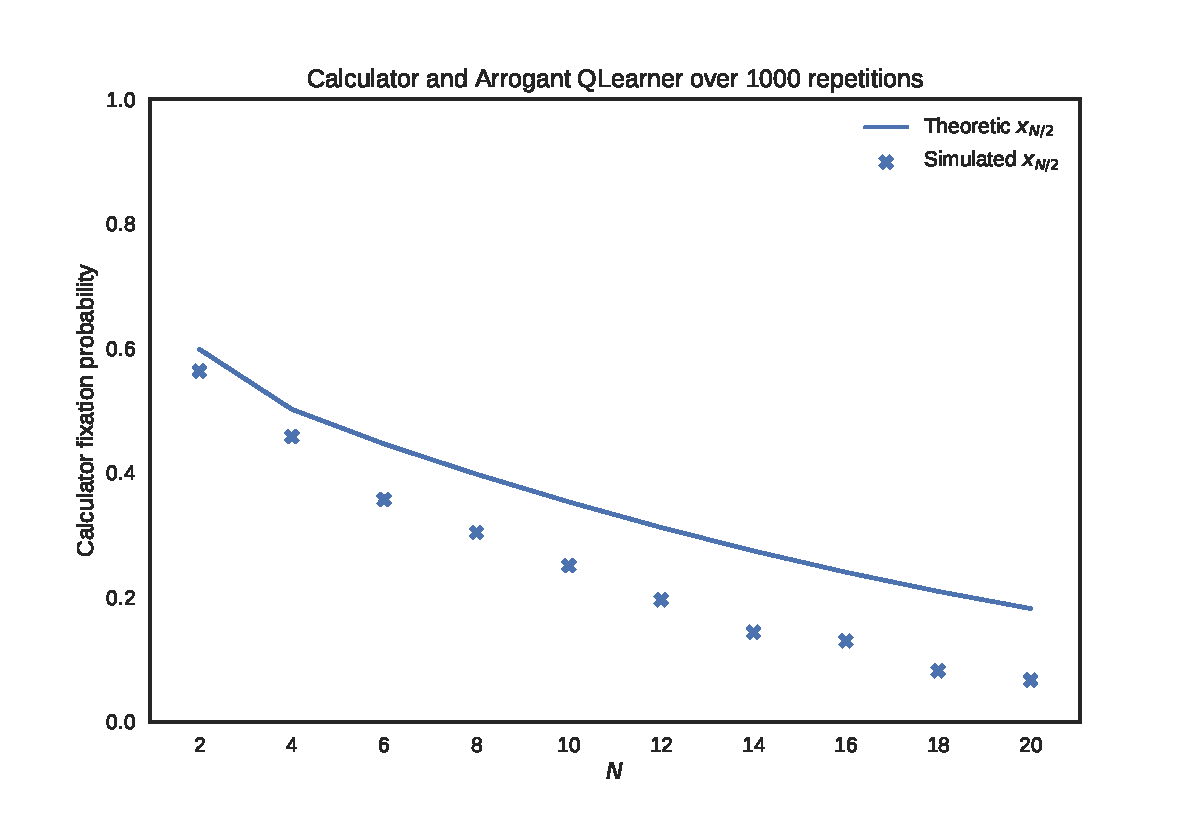
\includegraphics[width=.8\textwidth]{./img/Calculator_v_Arrogant_QLearner.pdf}
        \caption{Calculator and Arrogant Q learner}
    \end{subfigure}%
    ~
    \begin{subfigure}[t]{.3\textwidth}
        \centering
        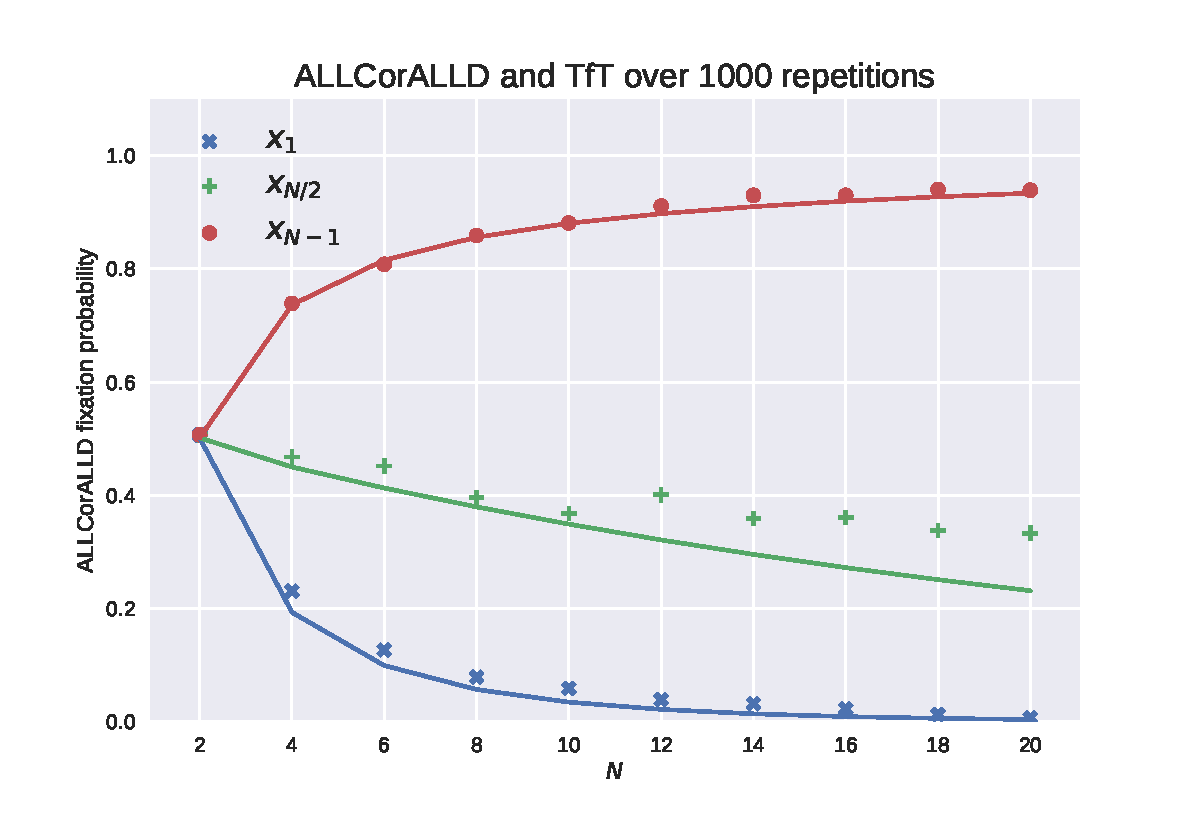
\includegraphics[width=.8\textwidth]{./img/ALLCorALLD_v_TfT.pdf}
        \caption{All C or all D and Tit For Tat}
    \end{subfigure}%
    \caption{Comparison of theoretic and actual Moran Process
             fixation probabilities for \textbf{stochastic} strategies}
    \label{fig:comparison_stochastic}
\end{figure}

Figure~\ref{fig:comparison_stochastic} shows the fixation probabilities for
stochastic strategies. These are no longer a good match which highlights the
weakness of the analytical formulae that relies on the average payoffs. A
detailed analysis of the 164 strategies considered, using direct Moran processes
will be shown in the next Section.


\section{Empirical results}\label{sec:empirical_results}

% TODO Archive all data (Zenodo) and include details/reference here.

This section outlines the data analysis carried out:

\begin{itemize}
    \item Section~\ref{sec:two_individuals} considers the specific case of
        \(N=2\).
    \item Section~\ref{sec:strong_invaders} investigates the effect of
        population size on the ability of a strategy to invade another
        population. This will highlight how complex strategies with long
        memories outperform simpler strategies.
    \item Section~\ref{sec:strong_resistors} similarly investigates the
        ability to defend against an invasion.
    \item Section~\ref{sec:population_size} investigates the relationship
        between performance for differing population sizes.
    \item Section~\ref{sec:relative_fitness} calculates the relative fitness of all
        strategies.
\end{itemize}

\subsection{The special case of \(N=2\)}\label{sec:two_individuals}

When $N=2$ the Moran process is effectively a measure of the relative
mean payoffs over all possible matches between two players. The strategy
that scores higher than the other more often will fixate more often.

Overall the main fixation probabilities of interest are \(x_1\) and \(x_{N-1}\), these
reflect a strategy's ability to invade or resist invasion; for \(N=2\) these two cases
coincide. Figure~\ref{fig:boxplot_2} shows
all fixation probabilities for the strategies considered. This is summarised
in Table~\ref{tbl:summary_top_2}.

\begin{enumerate}
    \item The top strategy is the Collective Strategy (CS) which has a simple
        handshake mechanism (a cooperation followed by a defection on the first
        move). As long as the opponent plays the same handshake and does not
        defect in the future it cooperates. Otherwise it defects for all
        rounds~\cite{Li2009}. This strategy was specifically designed for
        evolutionary processes.
    \item The finite state machine strategy % TODO Perhaps refer to earlier
        % discussion in the methodology section about these FSM strategies
    \item The Defector: it always defects. As it has little potential
        interaction with itself, recall that \(N=2\) is considered, its
        aggressiveness is rewarded.
    \item The Aggravater strategy which plays like Grudger (responding to any
        defections with unconditional defections throughout) however starts by
        playing 3 defections.
    \item Predator, a finite state machine described in~\cite{Ashlock2006}.
\end{enumerate}


\begin{figure}[!hbtp]
    \centering
    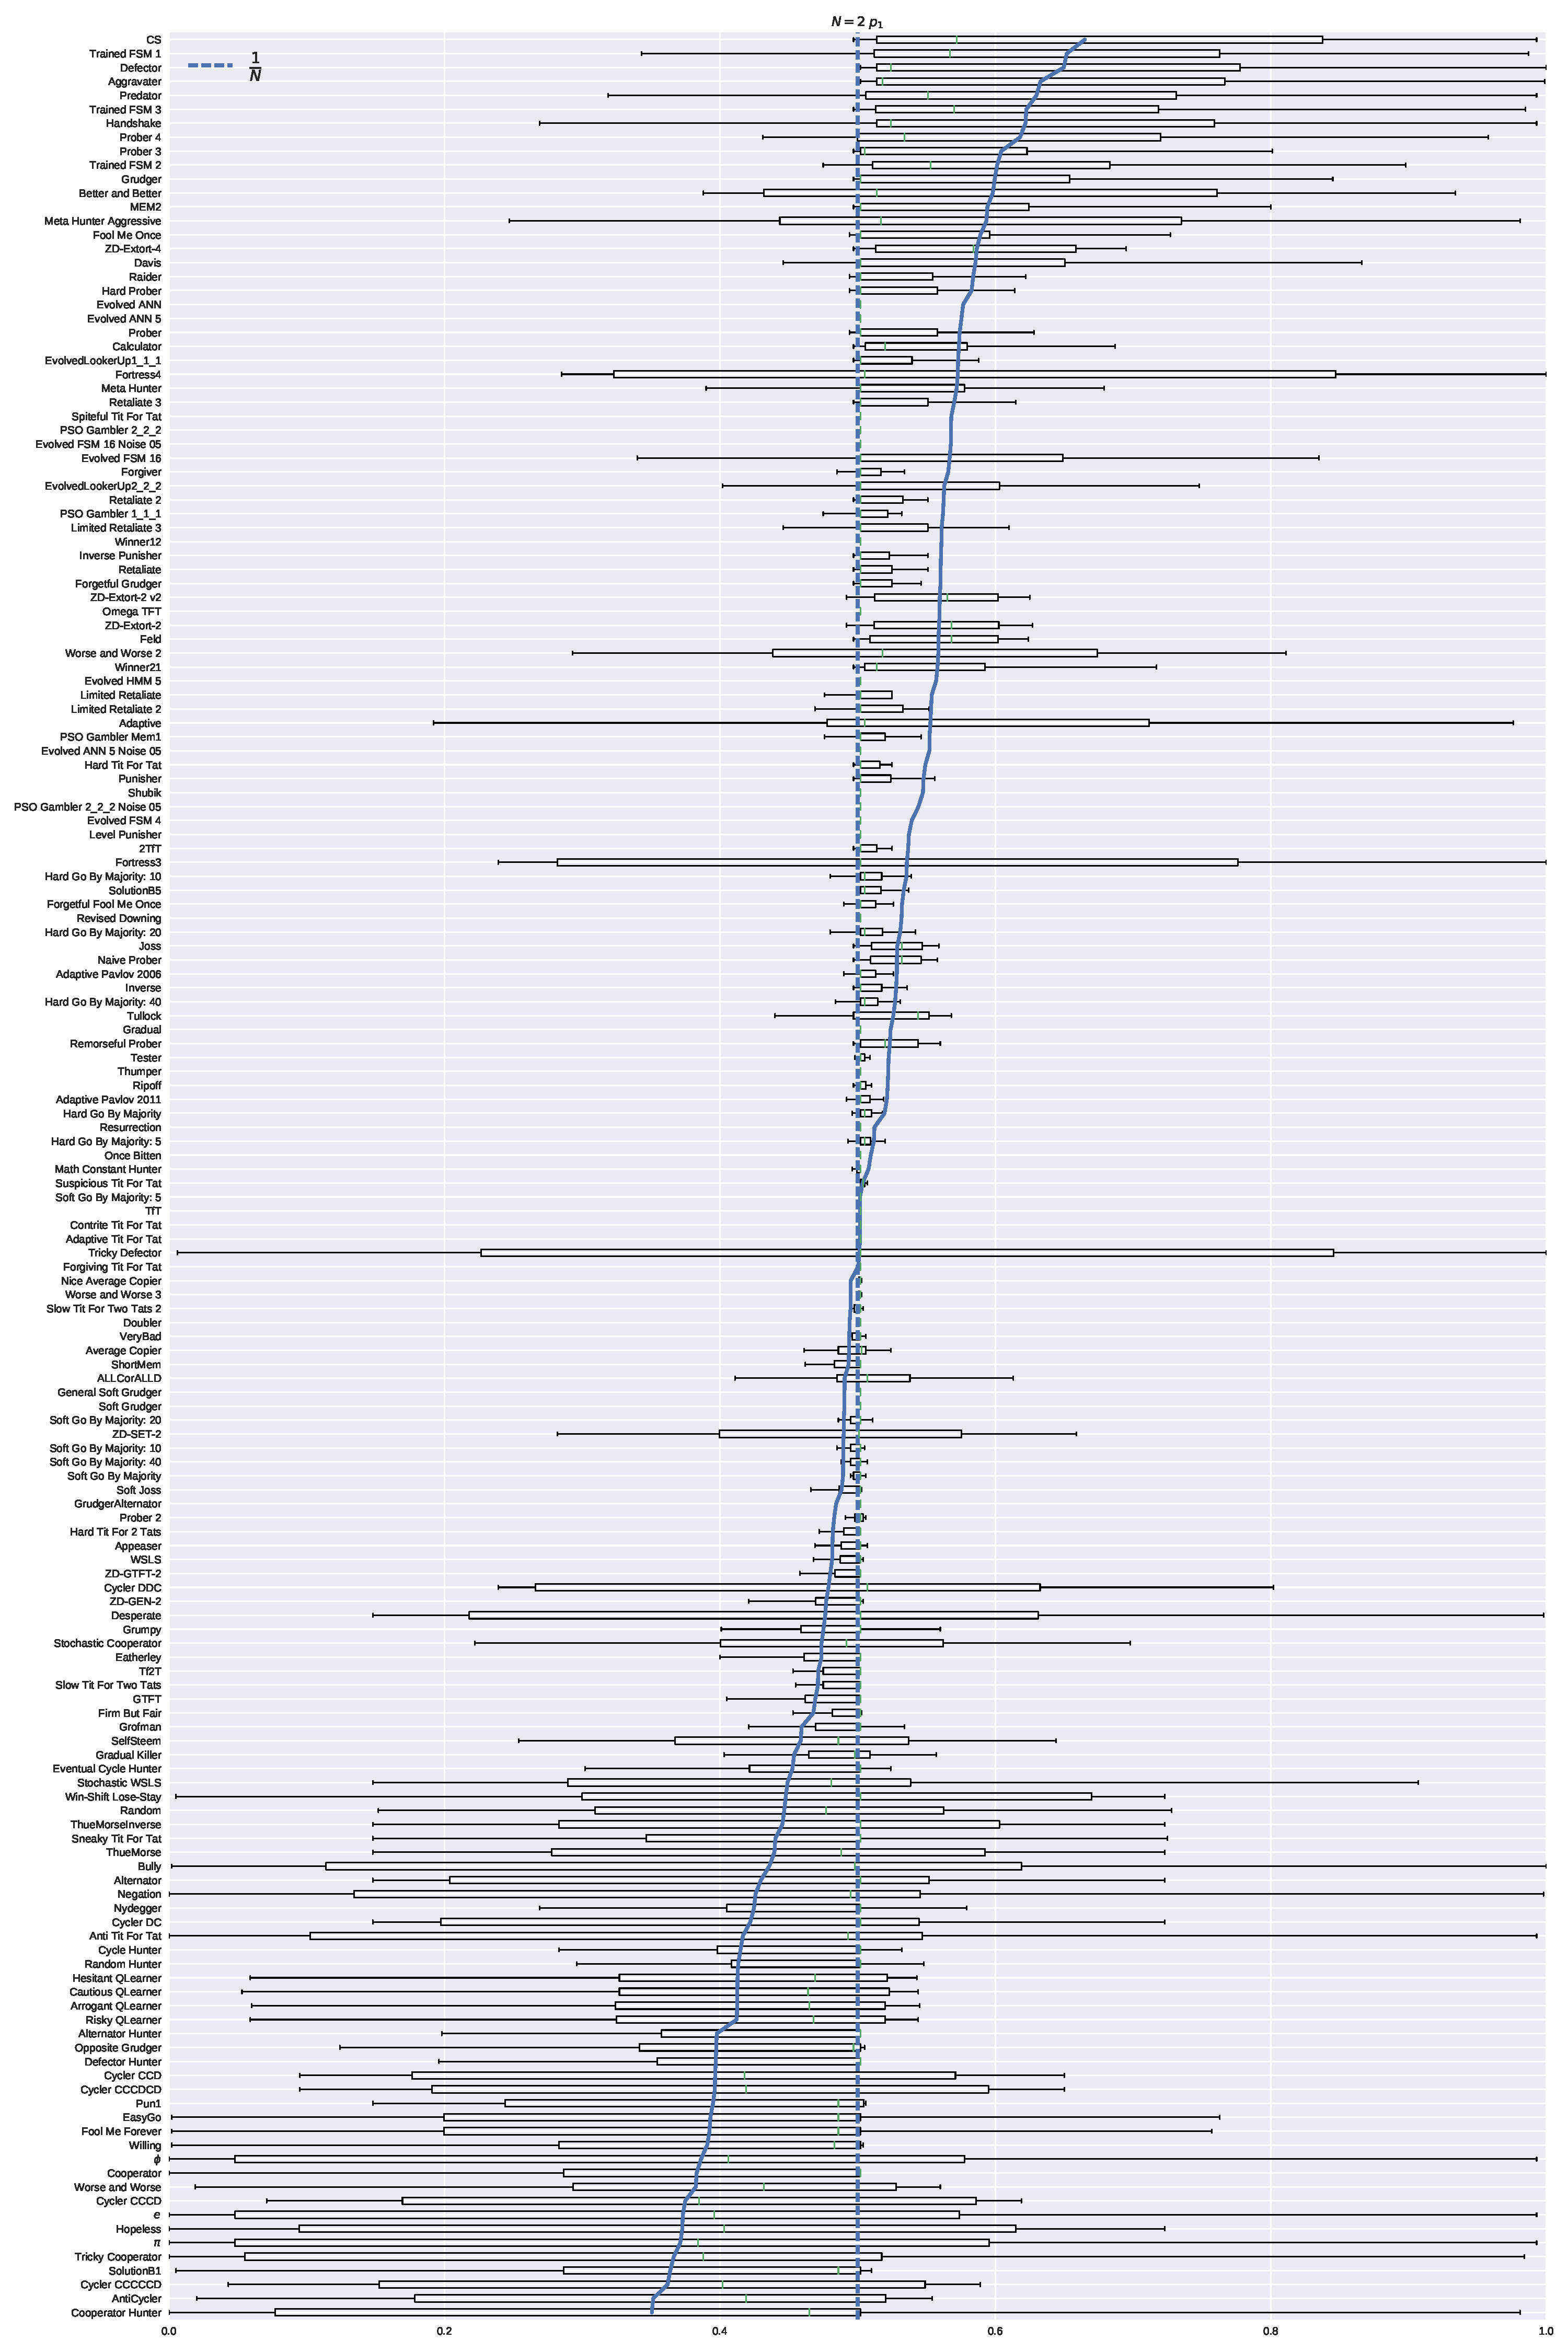
\includegraphics[height=.8\textheight]{./img/boxplot_2_invade.pdf}
    \caption{The fixation probabilities for \(N=2\)}
    \label{fig:boxplot_2}
\end{figure}

\begin{table}[!hbtp]
    \centering
    \begin{tabular}{lrrl}
\toprule
        Player &  Median $p_1$ &  Memory Depth & Stochastic \\
\midrule
   ZD-Extort-4 &         0.584 &             1 &       True \\
            CS &         0.572 &            \(\infty\) &      False \\
 Trained FSM 3 &         0.570 &             1 &      False \\
          Feld &         0.568 &           200 &       True \\
   ZD-Extort-2 &         0.568 &             1 &       True \\
\bottomrule
\end{tabular}

    \caption{Summary of top five strategies for \(N=2\)}
    \label{tbl:summary_top_2}
\end{table}

As will be demonstrated in Section~\ref{sec:population_size} the results for
\(N=2\) differ from those of larger $N$. Hence our results do not concur with
the literature which suggests that Zero Determinant strategies should be
effective for larger population sizes, but we note that those analysis run each
match to stationarity, while our matches run for a fixed number of rounds.

In the next sections we pay close attention to
strategies who are strong invaders/resistors.

\subsection{Strong invaders}\label{sec:strong_invaders}

In this section we focus on the ability of a mutant strategy to invade: the
probability of 1 individual of a given type successfully becoming fixated in a
population of \(N - 1\) other individuals, denoted by \(x_i\). The fixation
probabilities are shown in
Figures~\ref{fig:boxplot_3_invade},~\ref{fig:boxplot_7_invade}
and~\ref{fig:boxplot_14_invade} for \(N\in\{3, 7, 14\}\) showing the mean
fixation as well as the neutral fixation for each given scenario.

\begin{figure}[!hbtp]
    \centering
    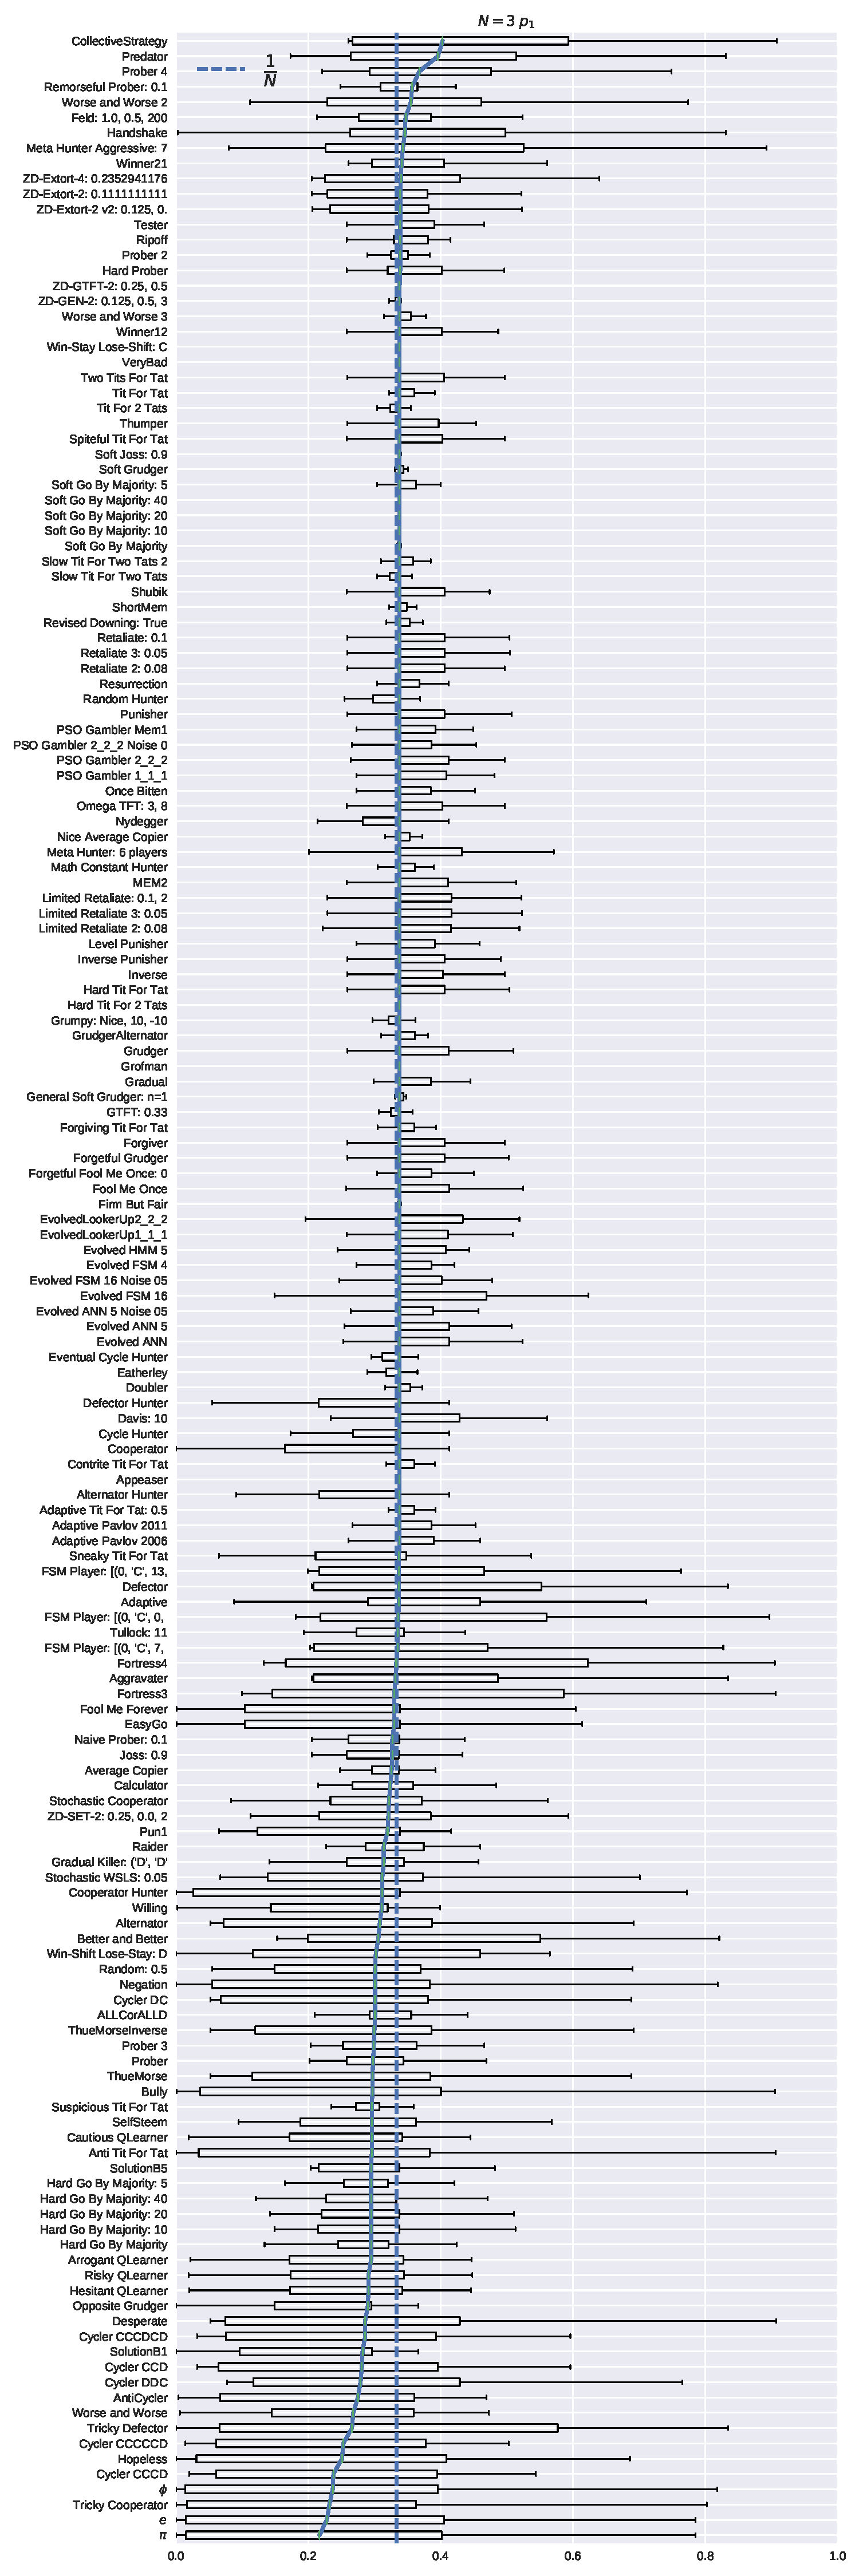
\includegraphics[height=.8\textheight]{./img/boxplot_3_invade.pdf}
    \caption{The fixation probability \(x_1\) for \(N=3\)}
    \label{fig:boxplot_3_invade}
\end{figure}

\begin{figure}[!hbtp]
    \centering
    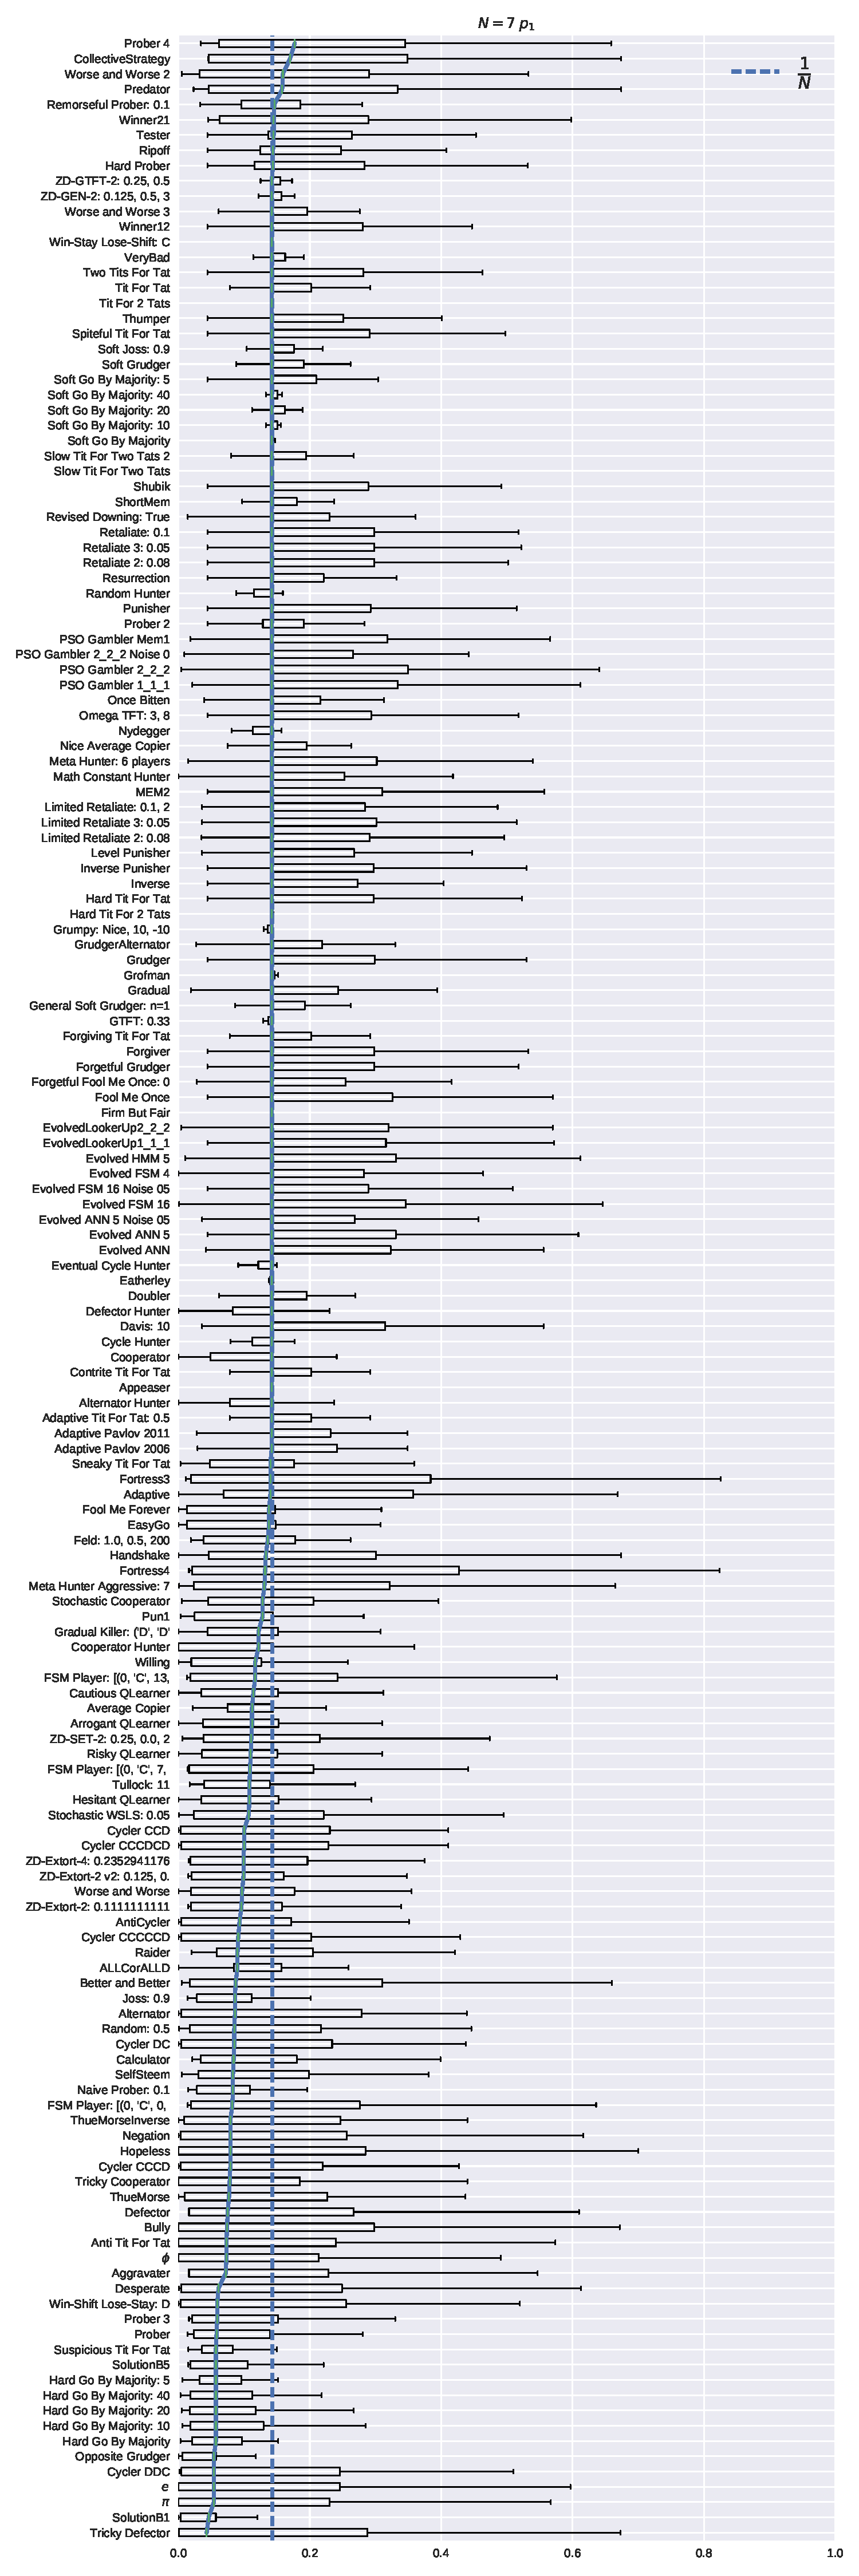
\includegraphics[height=.8\textheight]{./img/boxplot_7_invade.pdf}
    \caption{The fixation probability \(x_1\) for \(N=7\)}
    \label{fig:boxplot_7_invade}
\end{figure}

\begin{figure}[!hbtp]
    \centering
    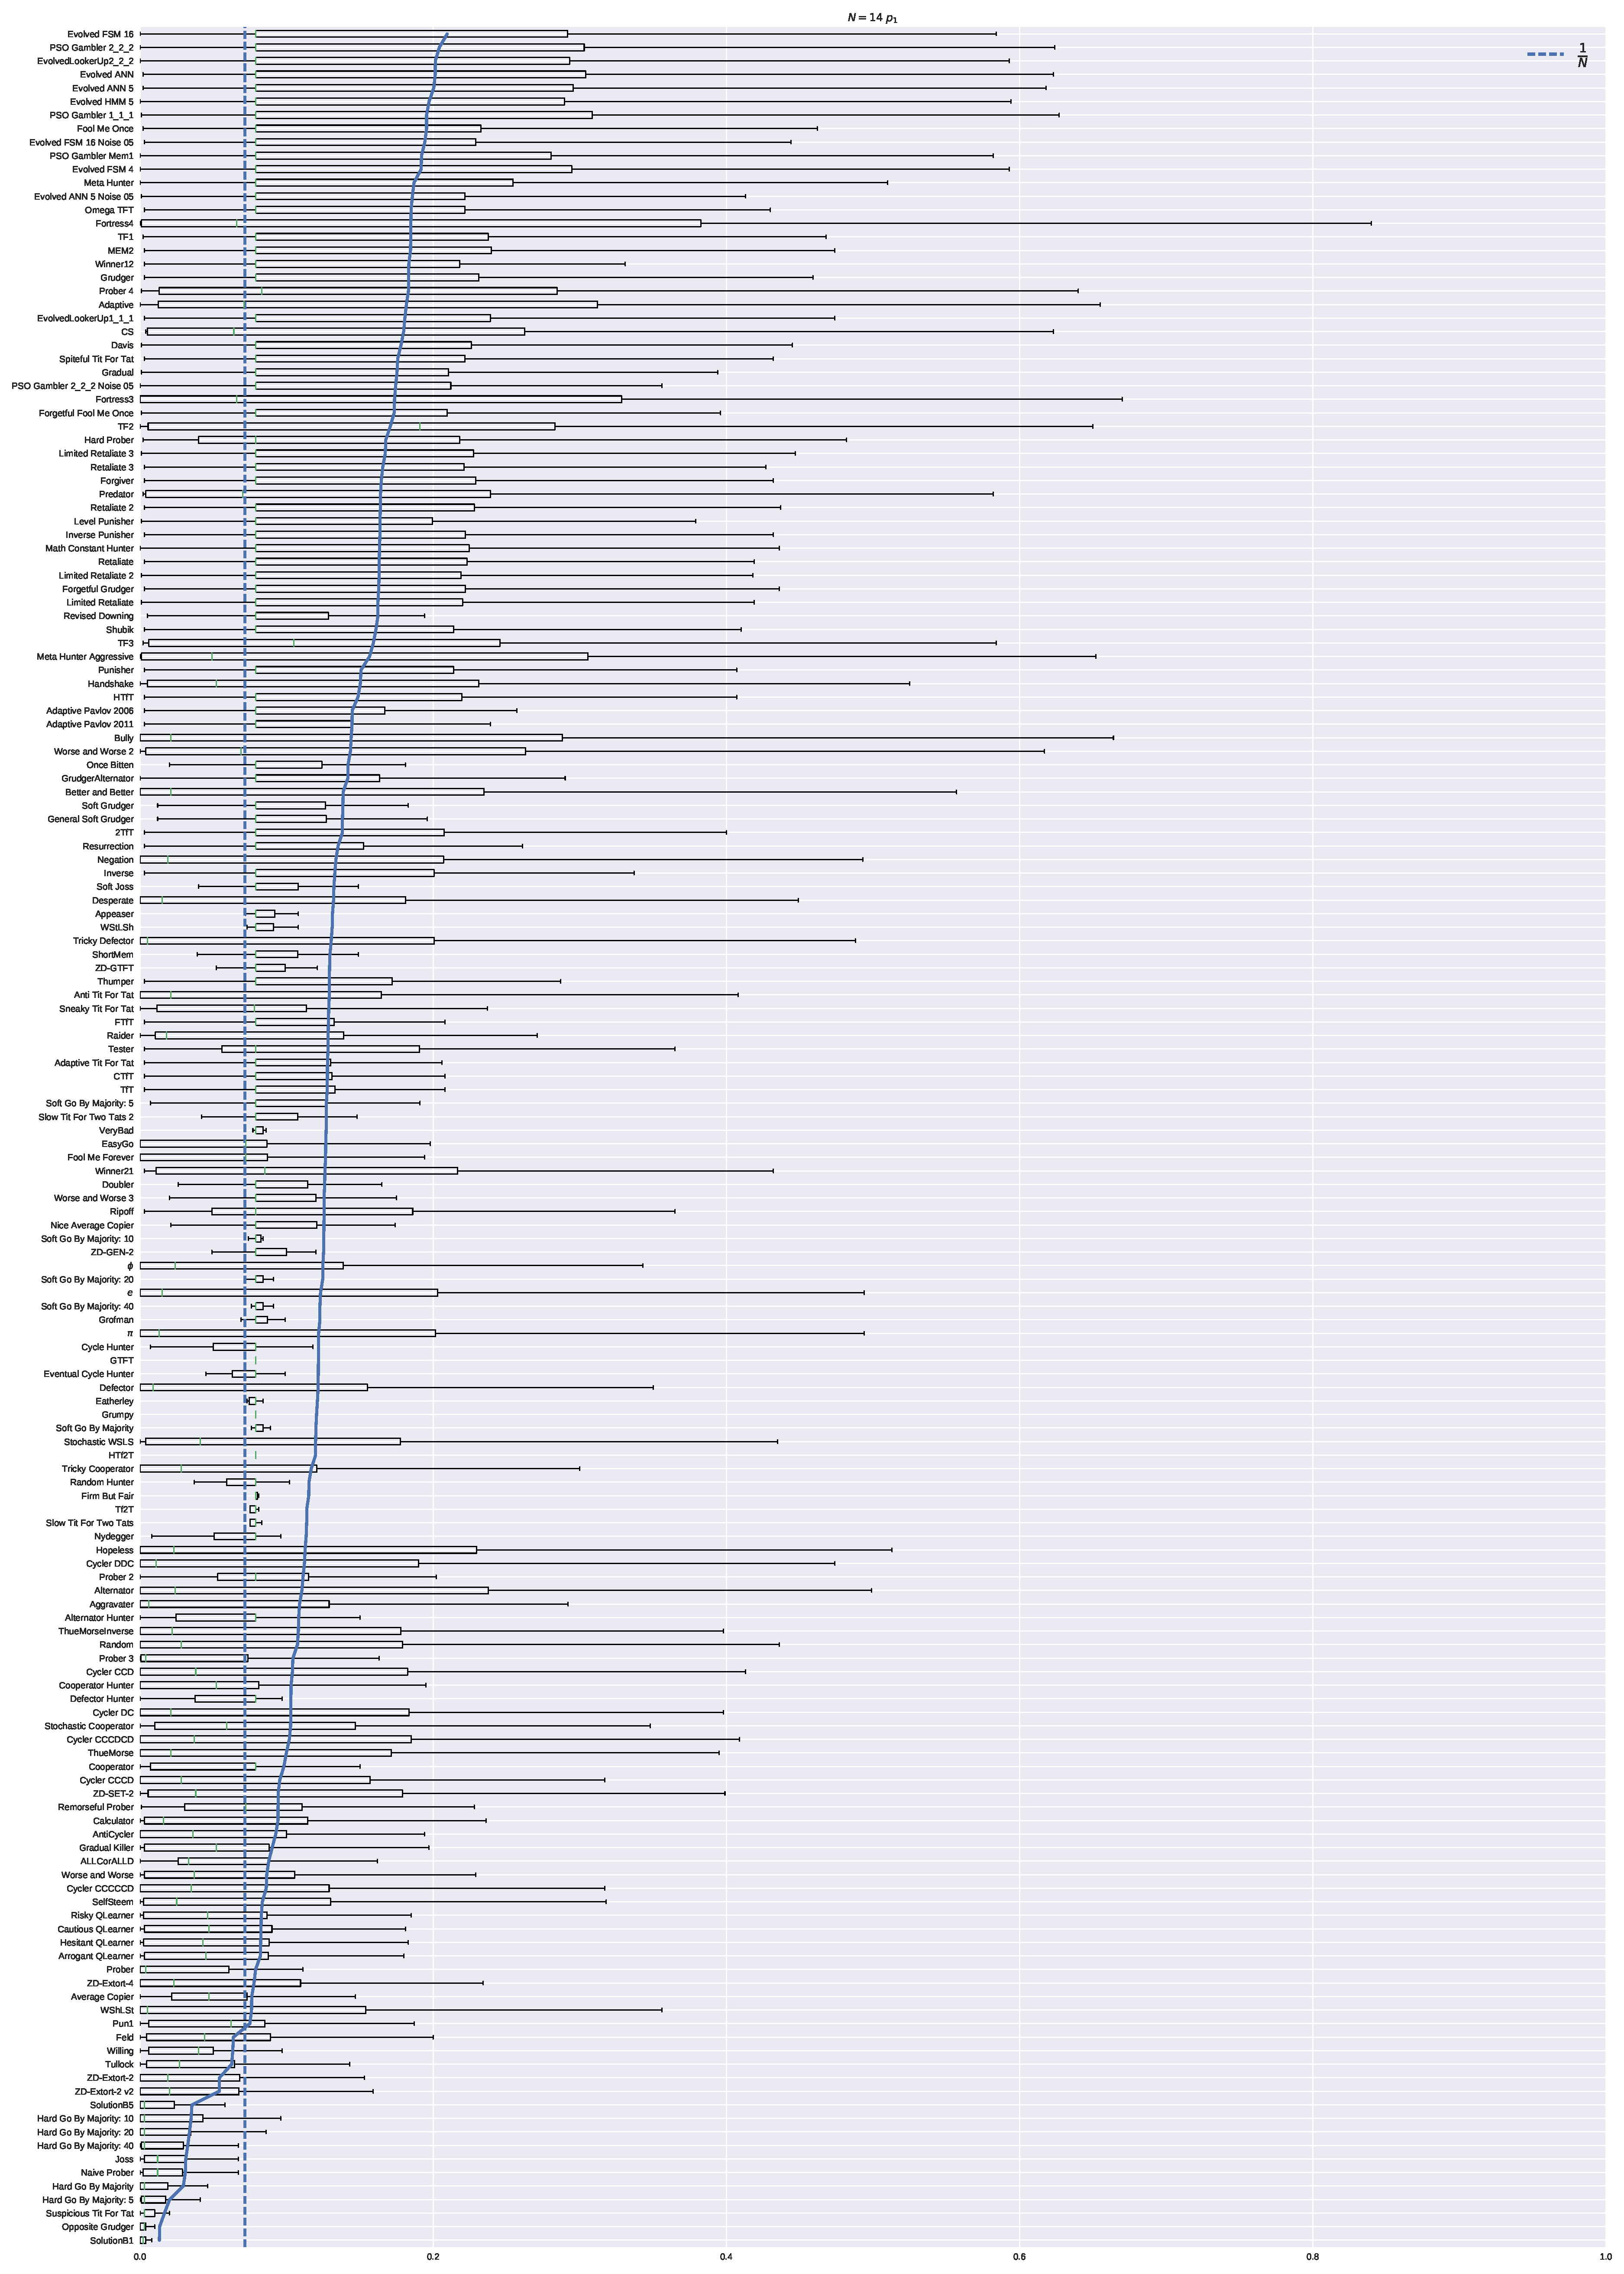
\includegraphics[height=.8\textheight]{./img/boxplot_14_invade.pdf}
    \caption{The fixation probability \(x_1\) for \(N=14\)}
    \label{fig:boxplot_14_invade}
\end{figure}


The top five strategies are given in Tables~\ref{tbl:top_five_invade}.

\begin{table}[!hbtp]
    \begin{subfigure}[t]{\textwidth}
        \centering
        \begin{tabular}{lrrl}
\toprule
   Player &  Mean $p_1$ &  Memory Depth & Stochastic \\
\midrule
       CS &    0.447761 &            \(\infty\) &      False \\
  Grudger &    0.431264 &            \(\infty\) &      False \\
     MEM2 &    0.427804 &            \(\infty\) &      False \\
      TF3 &    0.426736 &            16 &      False \\
 Prober 4 &    0.424215 &            \(\infty\) &      False \\
\bottomrule
\end{tabular}

        \caption{\(N=3\)}
    \end{subfigure}
    \begin{subfigure}[t]{\textwidth}
        \centering
        \begin{tabular}{llr}
\toprule
{} &                   Player &  Mean $p_1$ \\
\midrule
1  &           Evolved FSM 16 &      0.2523 \\
2  &        PSO Gambler 2\_2\_2 &      0.2467 \\
3  &             Fool Me Once &      0.2459 \\
4  &            Evolved ANN 5 &      0.2450 \\
5  &              Evolved ANN &      0.2449 \\
6  &     EvolvedLookerUp2\_2\_2 &      0.2443 \\
7  &                  Grudger &      0.2442 \\
8  &                     MEM2 &      0.2436 \\
9  &                      \textbf{TF3} &      0.2430 \\
10 &        PSO Gambler 1\_1\_1 &      0.2404 \\
11 &                       CS &      0.2395 \\
12 &  Evolved FSM 16 Noise 05 &      0.2394 \\
13 &            Evolved HMM 5 &      0.2390 \\
14 &              Meta Hunter &      0.2385 \\
15 &                    Davis &      0.2379 \\
16 &         PSO Gambler Mem1 &      0.2348 \\
\bottomrule
\end{tabular}

        \caption{\(N=7\)}
    \end{subfigure}
    \begin{subfigure}[t]{\textwidth}
        \centering
        \begin{tabular}{llrrrrrrr}
\toprule
{} &                   Player &    Min &   5th \% &    Mean &  Median &  95th \% &    Max &     Std \\
\midrule
1  &           Evolved FSM 16 &  0.000 &  0.0054 &  0.2096 &   0.079 &  0.7241 &  0.842 &  0.2172 \\
2  &        PSO Gambler 2\_2\_2 &  0.000 &  0.0113 &  0.2042 &   0.079 &  0.5940 &  0.842 &  0.2045 \\
3  &     EvolvedLookerUp2\_2\_2 &  0.000 &  0.0270 &  0.2014 &   0.079 &  0.6608 &  0.840 &  0.2097 \\
4  &              Evolved ANN &  0.002 &  0.0164 &  0.2014 &   0.079 &  0.5939 &  0.842 &  0.2074 \\
5  &            Evolved ANN 5 &  0.002 &  0.0505 &  0.2004 &   0.079 &  0.5940 &  0.834 &  0.2009 \\
6  &            Evolved HMM 5 &  0.000 &  0.0321 &  0.1972 &   0.079 &  0.5940 &  0.842 &  0.2034 \\
7  &        PSO Gambler 1\_1\_1 &  0.001 &  0.0455 &  0.1955 &   0.079 &  0.6150 &  0.841 &  0.1931 \\
8  &             Fool Me Once &  0.002 &  0.0058 &  0.1955 &   0.079 &  0.5940 &  0.842 &  0.2032 \\
9  &  Evolved FSM 16 Noise 05 &  0.003 &  0.0607 &  0.1943 &   0.079 &  0.5930 &  0.842 &  0.2005 \\
10 &         PSO Gambler Mem1 &  0.000 &  0.0517 &  0.1920 &   0.079 &  0.6118 &  0.841 &  0.1907 \\
11 &            Evolved FSM 4 &  0.000 &  0.0000 &  0.1918 &   0.079 &  0.5930 &  0.842 &  0.2049 \\
12 &              Meta Hunter &  0.000 &  0.0049 &  0.1869 &   0.079 &  0.5883 &  0.840 &  0.1882 \\
13 &   Evolved ANN 5 Noise 05 &  0.001 &  0.0303 &  0.1858 &   0.079 &  0.5930 &  0.840 &  0.1968 \\
14 &                Omega TFT &  0.003 &  0.0704 &  0.1849 &   0.079 &  0.5939 &  0.840 &  0.1927 \\
15 &                Fortress4 &  0.000 &  0.0000 &  0.1848 &   0.066 &  0.5919 &  0.840 &  0.2211 \\
16 &                      \textbf{TF3} &  0.002 &  0.0041 &  0.1846 &   0.079 &  0.6190 &  0.842 &  0.1890 \\
\bottomrule
\end{tabular}

        \caption{\(N=14\)}
    \end{subfigure}
    \caption{Properties of top five invaders}
    \label{tbl:top_five_invade}
\end{table}

It can be seen that apart from CS, none of the strategies
of Table~\ref{tbl:summary_top_2} perform well for \(N\in\{3, 7, 14\}\). The new
high performing strategies are:

\begin{itemize}
    \item Prober 4, complex strategy with an initial 20 move sequence of
        cooperations and defections~\cite{prison}. This initial sequence serves
        as approximate handshake.
    \item Grudger (which only performs well for \(N=3\)), starts by cooperating
        but will defect if at any point the opponent has defected.
    \item MEM2, an infinite memory strategy that switches between TfT, Tf2T, and
        Defector~\cite{Li2014}.
    \item Fool Me Once, forgives one defection but defects forever once a second
        defection takes place.
    \item  PSO Gambler and Evolved Lookerup 2 2 2: are strategies that make use
        of a lookup table mapping the first 2 moves of the opponent as well as
        the last 2 moves of both players to an action. The PSO gambler is a
        stochastic version which maps those states to probabilities of
        cooperating. The lookerup was described in \cite{Knight2016}.
	\item The evolved ANN strategies are neural networks that map a number of
		attributes (first move, number of cooperations, last move etc\dots) to
		an action. Both of these have been trained using an evolutionary
		algorithm and the ANN 5 was trained to perform well in a noisy
		tournament.
	\item The Evolved FSM 16, is a 16 state finite machine strategy that has
		been trained using an evolutionary algorithm.
\end{itemize}

As well as noting that the memory length and complexity of these strategies are
much greater than one, it is interesting to note that none of them are akin to
memory one strategies. Only one is stochastic.

\subsection{Strong resistors}\label{sec:strong_resistors}

In addition to identifying good invaders, we also identify strategies
resistant to invasion by other strategies by examining the distribution
of $x_{N-1}$ for each strategy. Note that this is equivalent to
looking at $x_1$ for all opponents.

The fixation
probabilities are shown in
Figures~\ref{fig:boxplot_3_resist},~\ref{fig:boxplot_7_invade}
and~\ref{fig:boxplot_14_resist} for \(N\in\{3, 7, 14\}\) showing the mean
fixation as well as the neutral fixation for each given scenario.

\begin{figure}[!hbtp]
    \centering
    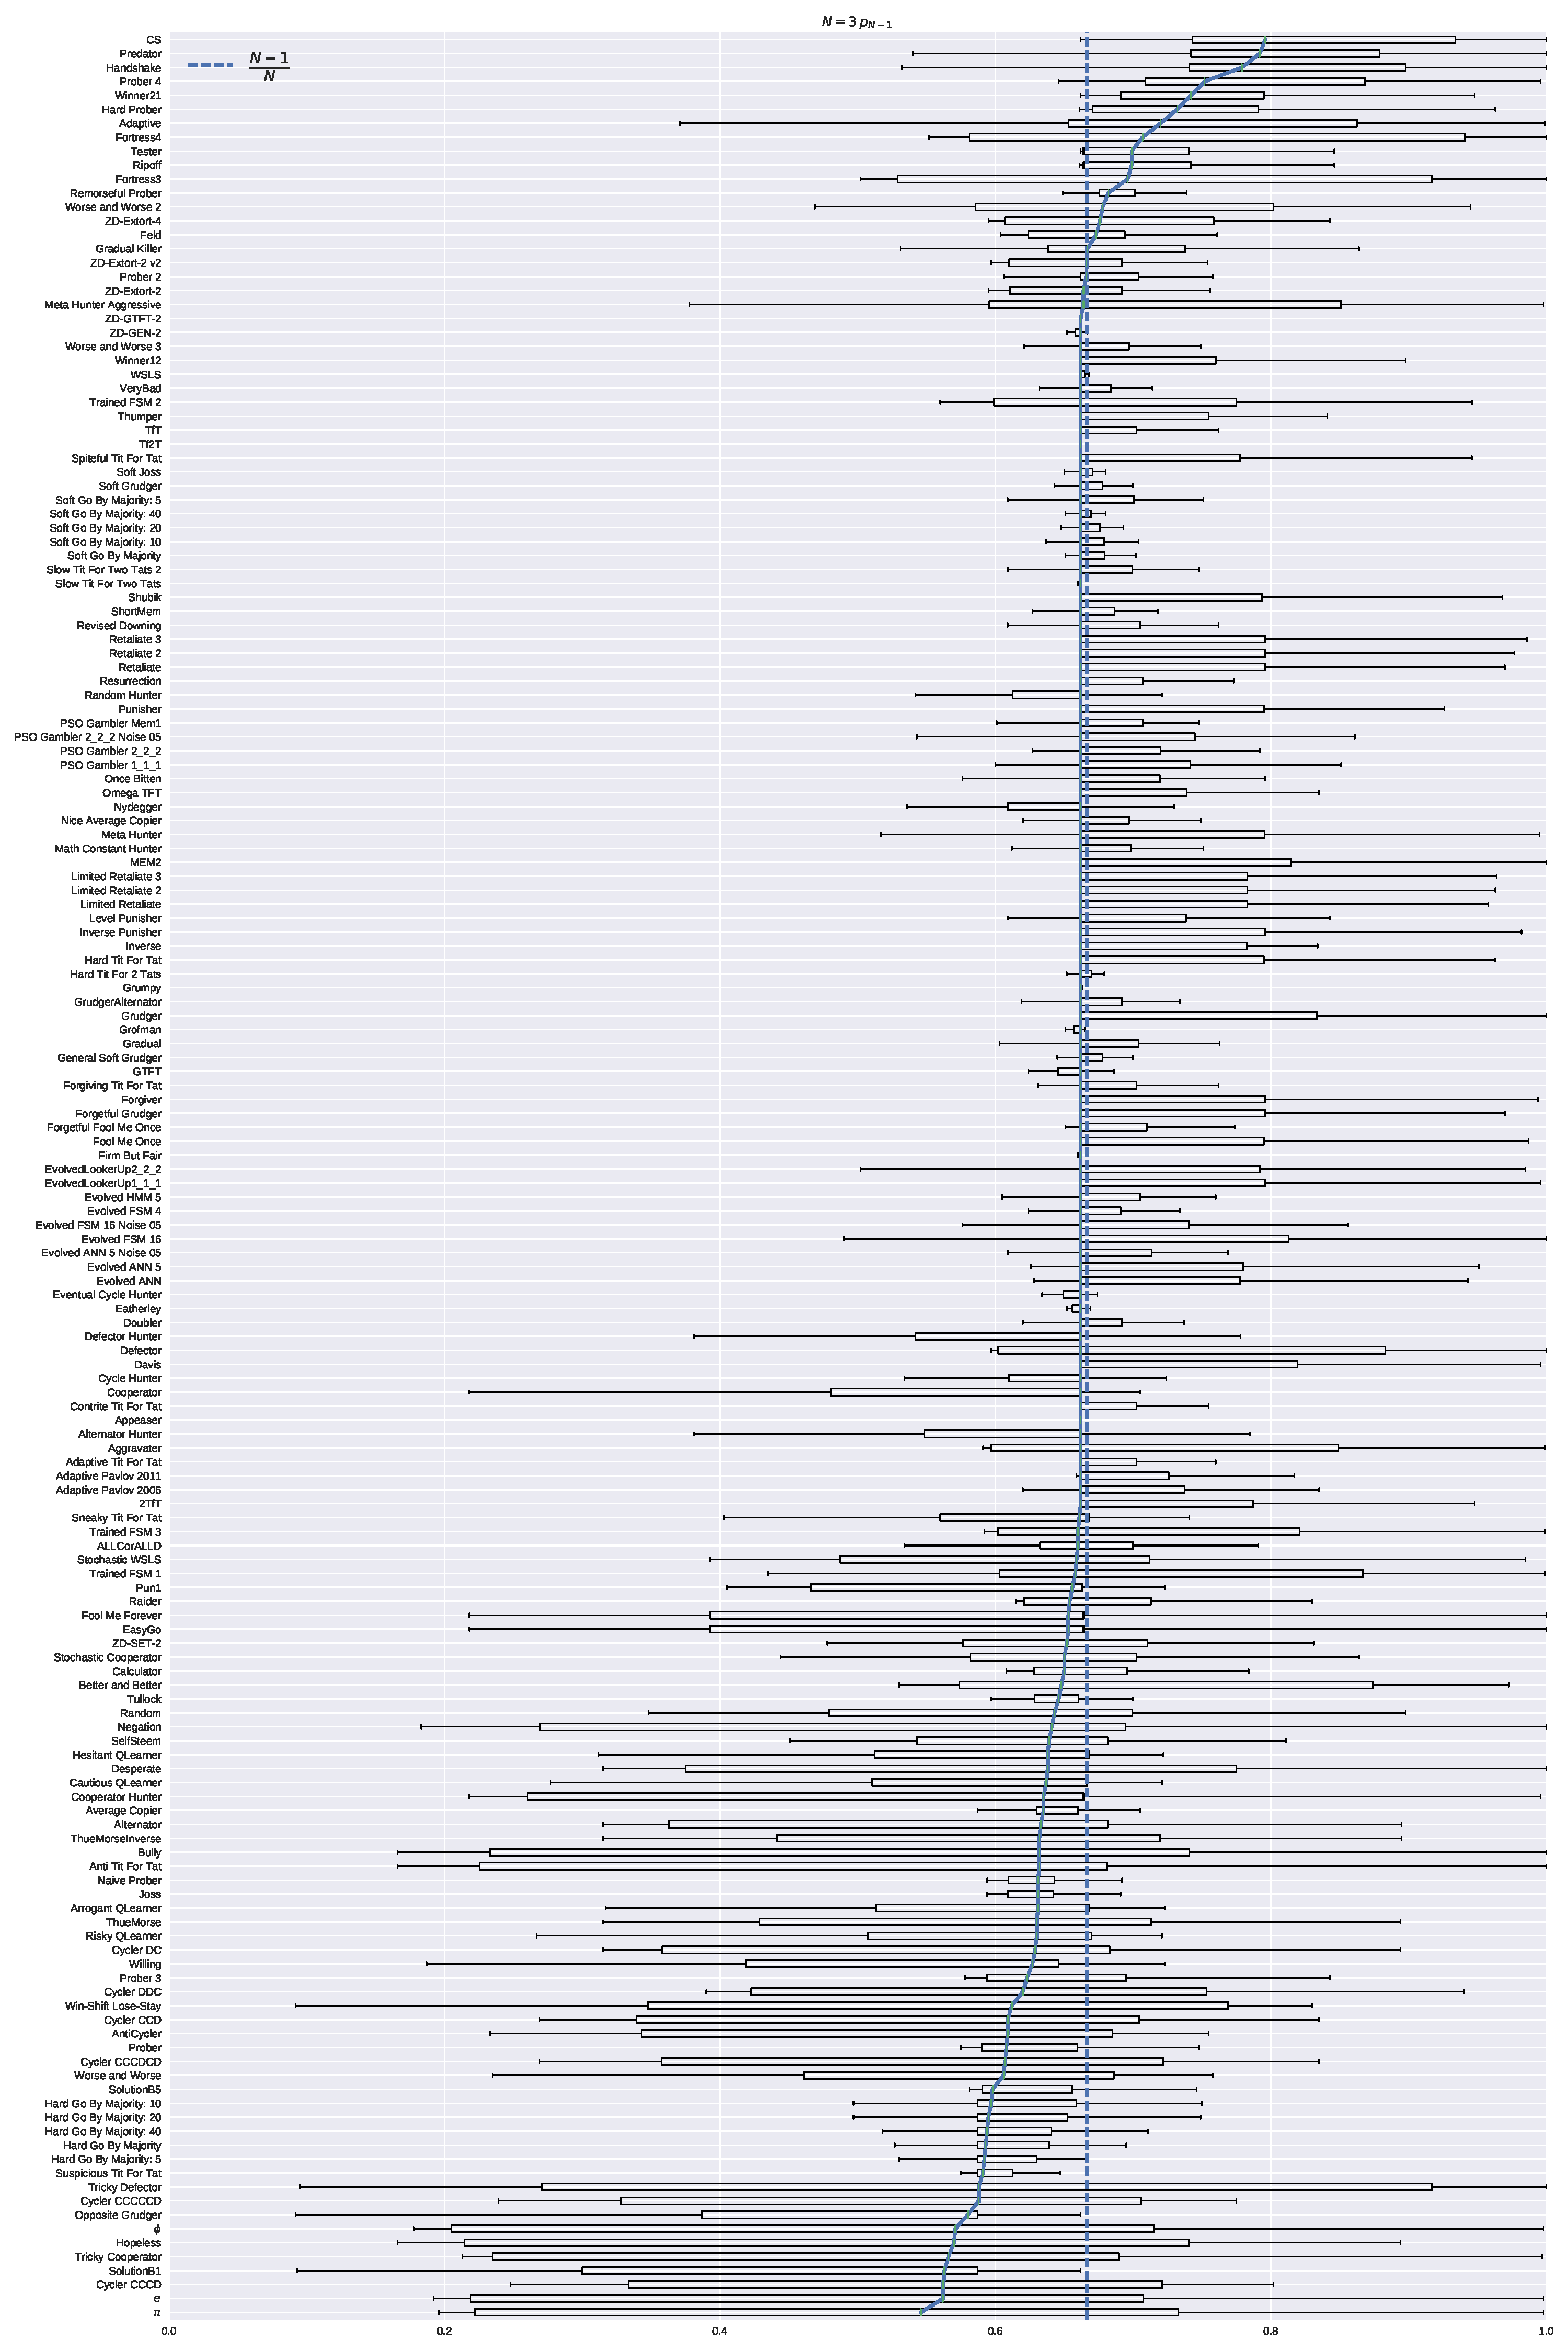
\includegraphics[height=.8\textheight]{./img/boxplot_3_resist.pdf}
    \caption{The fixation probability \(x_{N-1}\) for \(N=3\)}
    \label{fig:boxplot_3_resist}
\end{figure}

\begin{figure}[!hbtp]
    \centering
    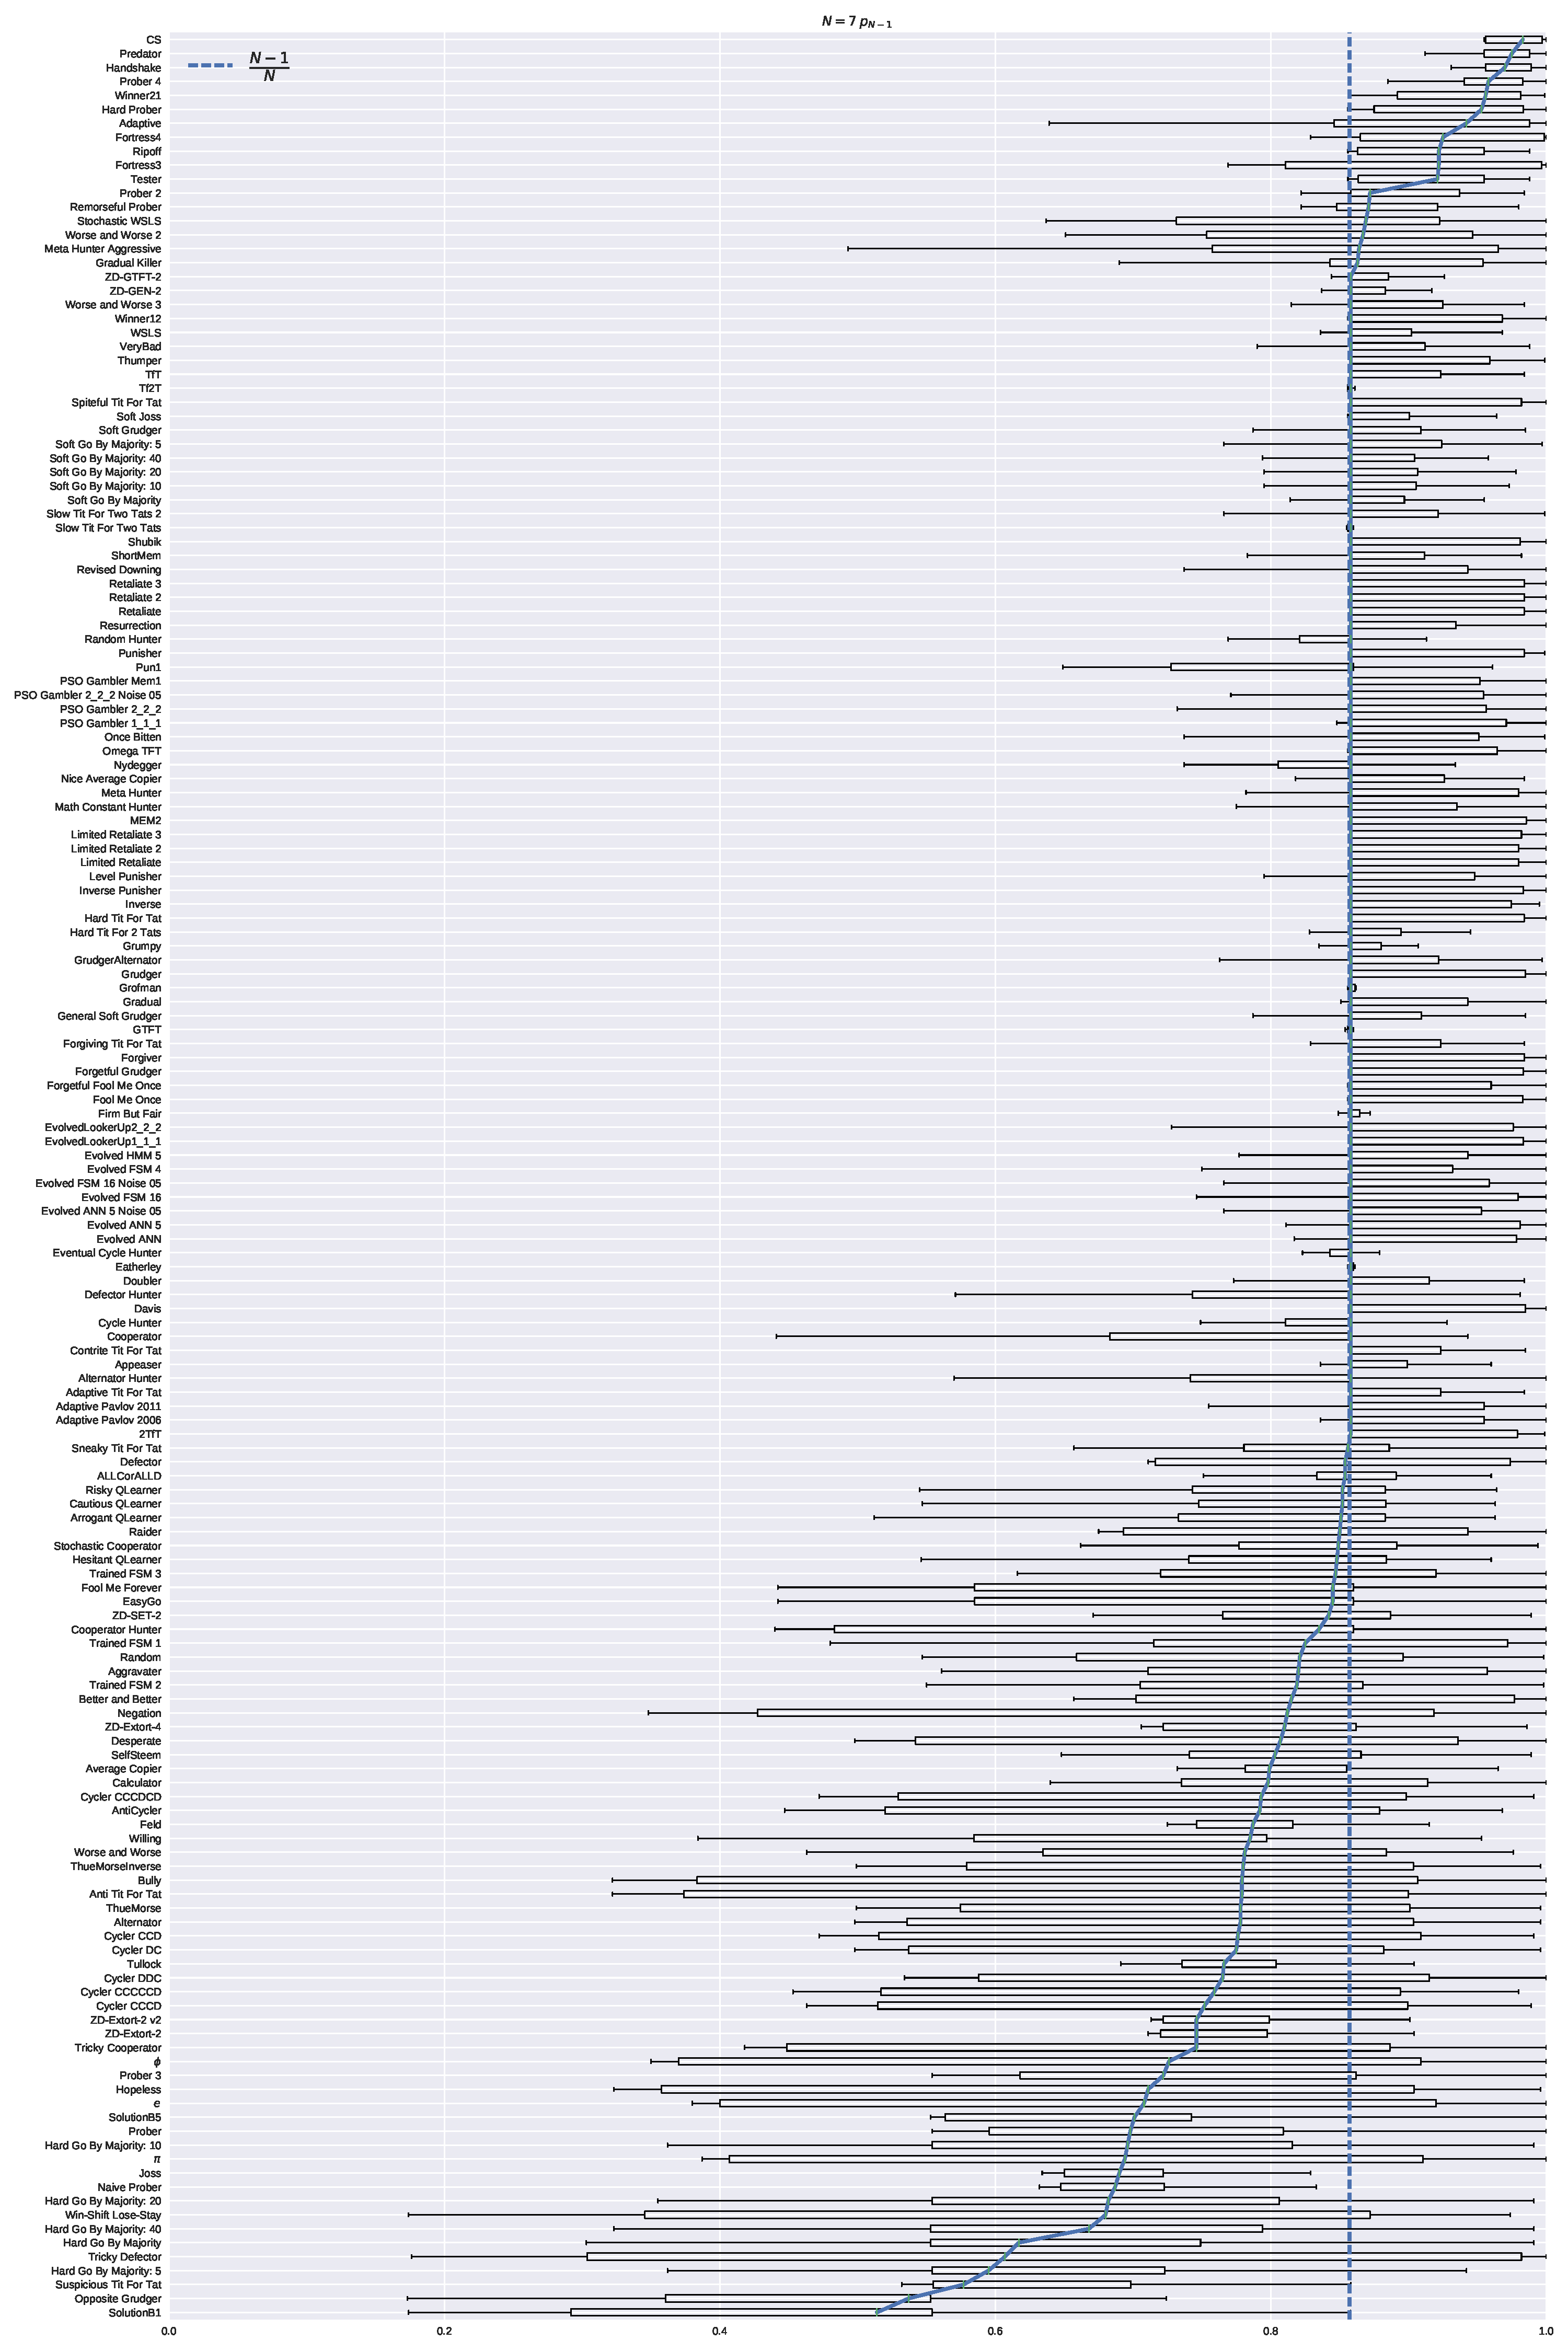
\includegraphics[height=.8\textheight]{./img/boxplot_7_resist.pdf}
    \caption{The fixation probability \(x_{N-1}\) for \(N=7\)}
    \label{fig:boxplot_6_resist}
\end{figure}

\begin{figure}[!hbtp]
    \centering
    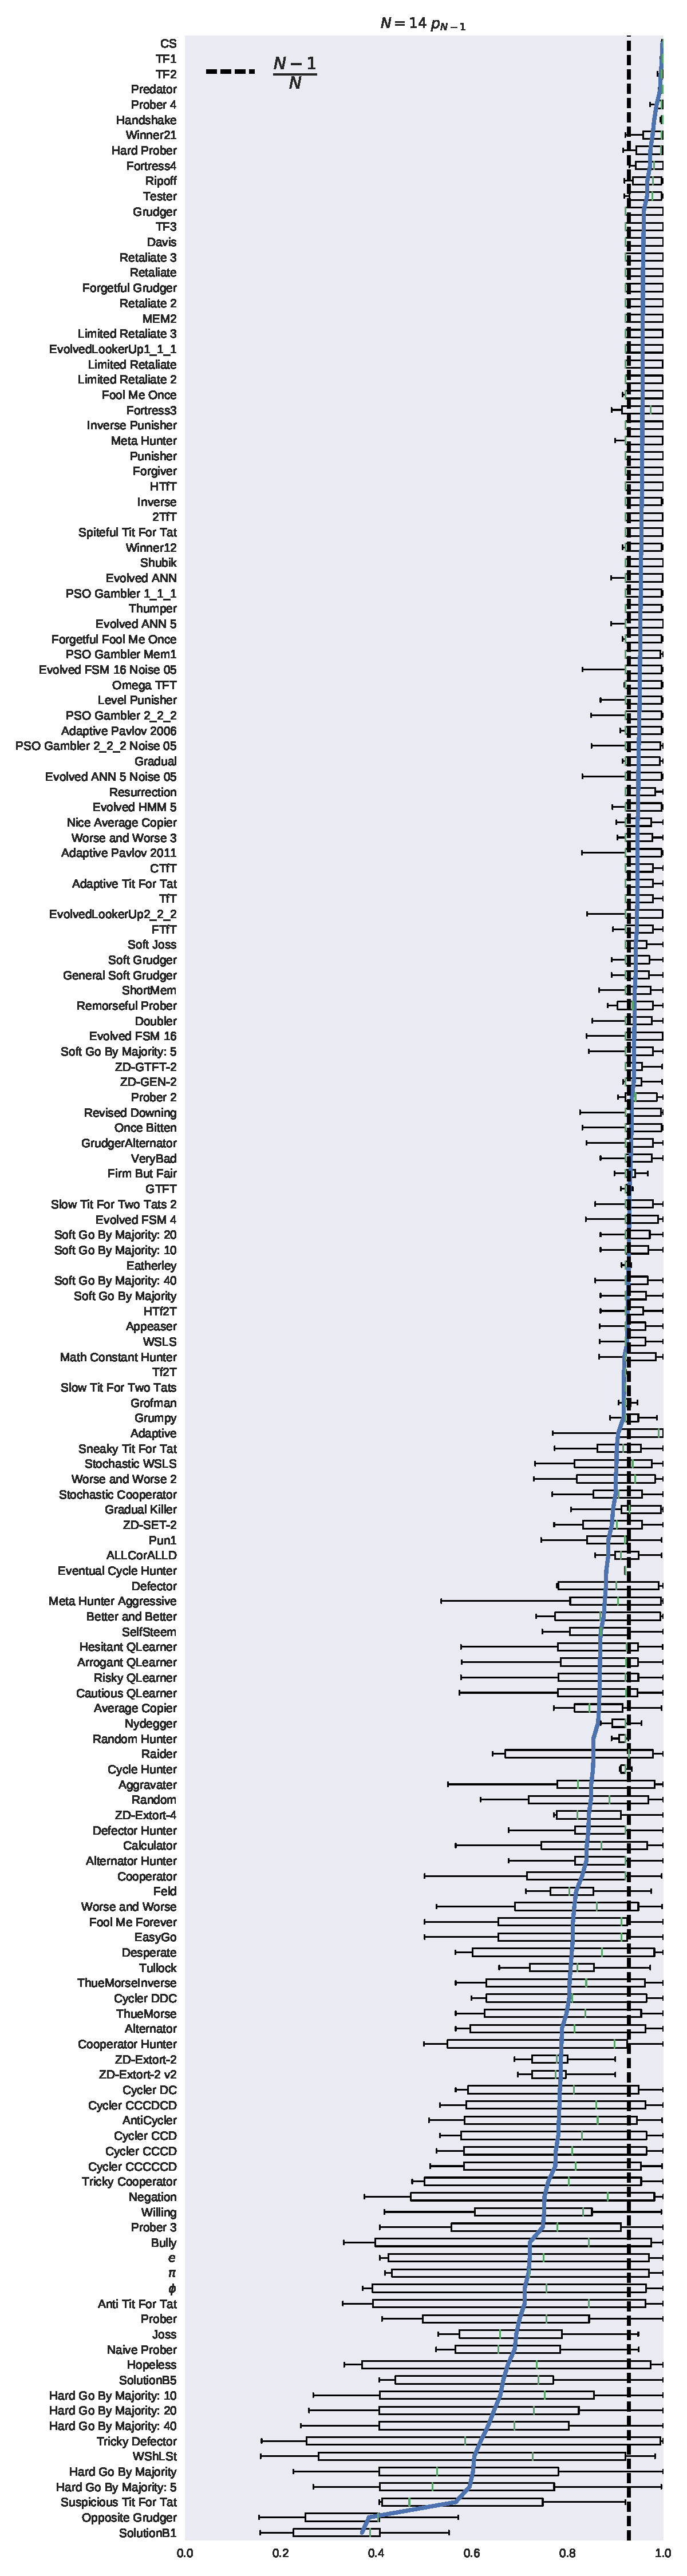
\includegraphics[height=.8\textheight]{./img/boxplot_14_resist.pdf}
    \caption{The fixation probability \(x_{N-1}\) for \(N=14\)}
    \label{fig:boxplot_14_resist}
\end{figure}

Table~\ref{tbl:top_five_resist} shows the top five strategies when ranked
according to \(x_{N-1}\) for \(N\in\{3, 7, 14\}\).
Once again none of the short memory strategies from
Section~\ref{sec:two_individuals} perform well for high \(N\).

\begin{table}[!hbtp]
    \begin{subfigure}[t]{\textwidth}
        \centering
        \begin{tabular}{lrrl}
\toprule
    Player &  Mean $p_{N-1}$ &  Memory Depth & Stochastic \\
\midrule
        CS &        0.835859 &            \(\infty\) &      False \\
  Predator &        0.812129 &             9 &      False \\
       TF3 &        0.808736 &             1 &      False \\
 Handshake &        0.801356 &            \(\infty\) &      False \\
       TF2 &        0.795736 &             1 &      False \\
\bottomrule
\end{tabular}

        \caption{\(N=3\)}
    \end{subfigure}
    \begin{subfigure}[t]{\textwidth}
        \centering
        \begin{tabular}{lrrl}
\toprule
    Player &  Mean $p_{N-1}$ &  Memory Depth & Stochastic \\
\midrule
        CS &        0.976491 &            \(\infty\) &      False \\
       TF3 &        0.971405 &             1 &      False \\
       TF2 &        0.967712 &             1 &      False \\
  Predator &        0.967687 &             9 &      False \\
 Handshake &        0.954650 &            \(\infty\) &      False \\
\bottomrule
\end{tabular}

        \caption{\(N=7\)}
    \end{subfigure}
    \begin{subfigure}[t]{\textwidth}
        \centering
        \begin{tabular}{lrrl}
\toprule
    Player &  Mean $p_{N-1}$ &  Memory Depth & Stochastic \\
\midrule
        CS &        0.998491 &            \(\infty\) &      False \\
  Predator &        0.994147 &             9 &      False \\
  Prober 4 &        0.986994 &            \(\infty\) &      False \\
 Handshake &        0.979761 &            \(\infty\) &      False \\
  Winner21 &        0.977853 &             2 &      False \\
\bottomrule
\end{tabular}

        \caption{\(N=14\)}
    \end{subfigure}
    \caption{Properties of top five resistors}
    \label{tbl:top_five_resist}
\end{table}

There are 3 strategies that are only top performers in \(x_{N-1}\):

\begin{itemize}
    \item Handshake: a slightly less aggressive version of the Collective
        strategy \cite{robson1989}. As long as the initial sequence is played
        then it cooperates. Thus it will do well in a population consisting of
        many members of itself: just as the Collective strategy does. However it
        is not aggressive enough to invade other populations.
    \item Winner 21: a strategy that makes its decision deterministically based
        on 1 round of its own strategy and 2 of the opponent's strategy
        \cite{Mathieu2015}.
	\item Predator: a finite state machine described in~\cite{Ashlock2006}
\end{itemize}

Interestingly none of these strategies are stochastic: this is explained by
the need of strategies to have a steady hand when interacting with their own
kind. In essence: acting stochastically increase the chance of friendly fire.
However we note that it is possible to design a strategy with a ``stochastic
handshake'' \cite{Lee2015}.

It is evident through
Sections~\ref{sec:two_individuals},~\ref{sec:strong_invaders}
and~\ref{sec:strong_resistors} that performance of strategies not only depends
on the initial population distribution but also that there seems to be a
difference depending on whether or not \(N>2\). This will be explored further in
the next section.

\subsection{The effect of population size}\label{sec:population_size}

Figures~\ref{fig:ranks_v_size_invade},~\ref{fig:ranks_v_size_resist}
and~\ref{fig:ranks_v_size_coexist} show the median rank of each strategy against
population size. For all starting populations \(i\in\{1, N/2, N-1\}\) the ranks
of strategies are relatively stable across the different values of \(N>2\)
however for \(N=2\) there is a distinct difference. This confirms what has been
discussed in previous sections.

Tables~\ref{tbl:ranks_v_size_invade},~\ref{tbl:ranks_v_size_resist}
and~\ref{tbl:ranks_v_size_coexist} show the same information for the strategies
that rated high for \(N=2\) and \(N=14\).

\begin{figure}[!hbtp]
    \centering
    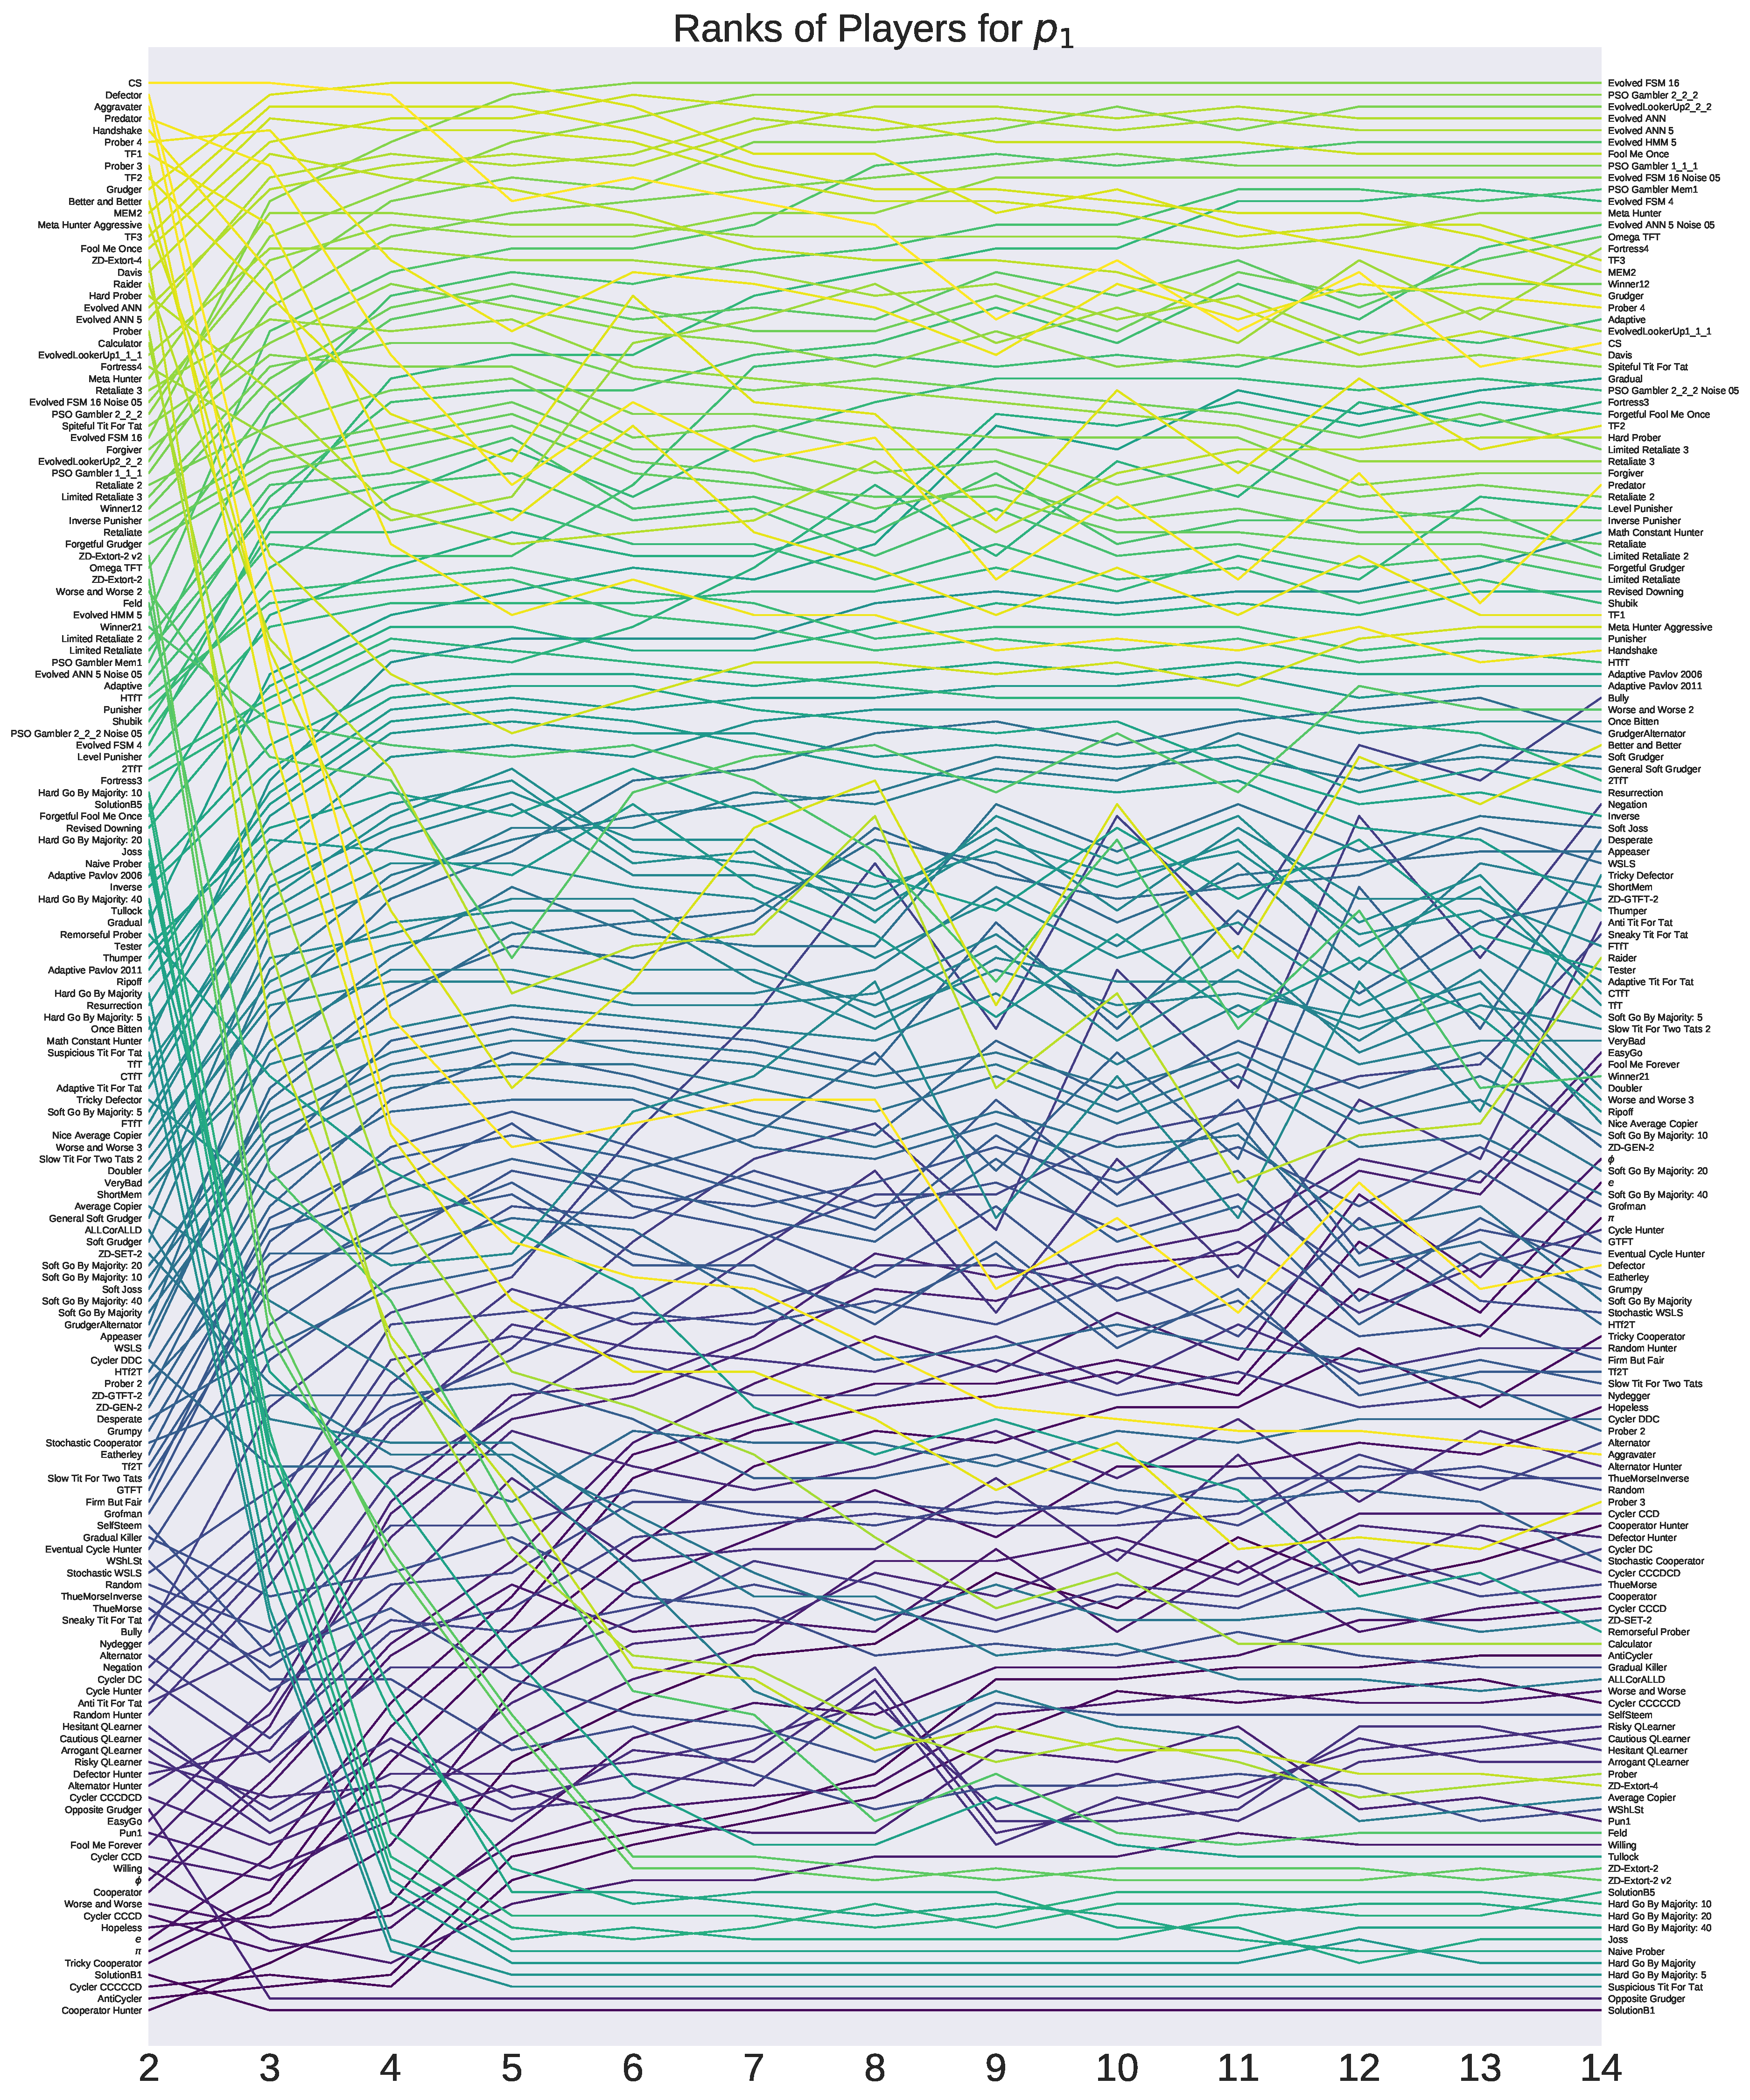
\includegraphics[height=.9\textheight]{./img/average_rank_vs_population_size_invade.pdf}
    \caption{Ranks of all strategies according to \(x_1\) for different
    population sizes}
    \label{fig:ranks_v_size_invade}
\end{figure}

\begin{table}[!hbtp]
    \centering
    \scriptsize
    \begin{tabular}{lrrrrrrrrrrrrr}
\toprule
               Player &     2 &     3 &     4 &     5 &      6 &      7 &      8 &      9 &     10 &     11 &     12 &     13 &     14 \\
\midrule
                   CS &   1.0 &   1.0 &   2.0 &   8.0 &    4.0 &    9.0 &   12.0 &   20.0 &   14.0 &   21.0 &   15.0 &   23.0 &   22.0 \\
        Trained FSM 1 &   2.0 &  29.0 &  55.0 &  71.0 &   67.0 &   57.0 &   54.0 &   71.0 &   60.0 &   68.0 &   53.0 &   59.0 &   53.0 \\
             Defector &   3.0 &  41.0 &  75.0 &  88.0 &   86.0 &   84.0 &   85.0 &   99.0 &   94.0 &  104.0 &   90.0 &  100.0 &   96.0 \\
           Aggravater &   4.0 &  48.0 &  88.0 &  98.0 &  101.0 &  102.0 &  107.0 &  112.0 &  111.0 &  114.0 &  113.0 &  113.0 &  116.0 \\
             Predator &   5.0 &   6.0 &  22.0 &  33.0 &   25.0 &   29.0 &   29.0 &   41.0 &   32.0 &   41.0 &   31.0 &   41.0 &   33.0 \\
       Evolved FSM 16 &  31.0 &  10.0 &   8.0 &   4.0 &    1.0 &    1.0 &    1.0 &    1.0 &    1.0 &    1.0 &    1.0 &    1.0 &    1.0 \\
    PSO Gambler 2\_2\_2 &  29.0 &  12.0 &   9.0 &   7.0 &    8.0 &    4.0 &    2.0 &    2.0 &    2.0 &    2.0 &    2.0 &    2.0 &    2.0 \\
          Evolved ANN &  20.0 &   9.0 &   6.0 &   5.0 &    7.0 &    5.0 &    3.0 &    3.0 &    3.0 &    3.0 &    3.0 &    3.0 &    3.0 \\
        Evolved ANN 5 &  21.0 &   8.0 &   5.0 &   6.0 &    6.0 &    3.0 &    5.0 &    4.0 &    4.0 &    4.0 &    5.0 &    4.0 &    4.0 \\
 EvolvedLookerUp2\_2\_2 &  33.0 &  15.0 &  11.0 &  10.0 &    9.0 &    8.0 &    6.0 &    6.0 &    5.0 &    5.0 &    4.0 &    5.0 &    5.0 \\
\bottomrule
\end{tabular}

    \caption{Ranks of some strategies according to \(x_1\) for different
    population sizes}
    \label{tbl:ranks_v_size_invade}
\end{table}

\begin{figure}[!hbtp]
    \centering
    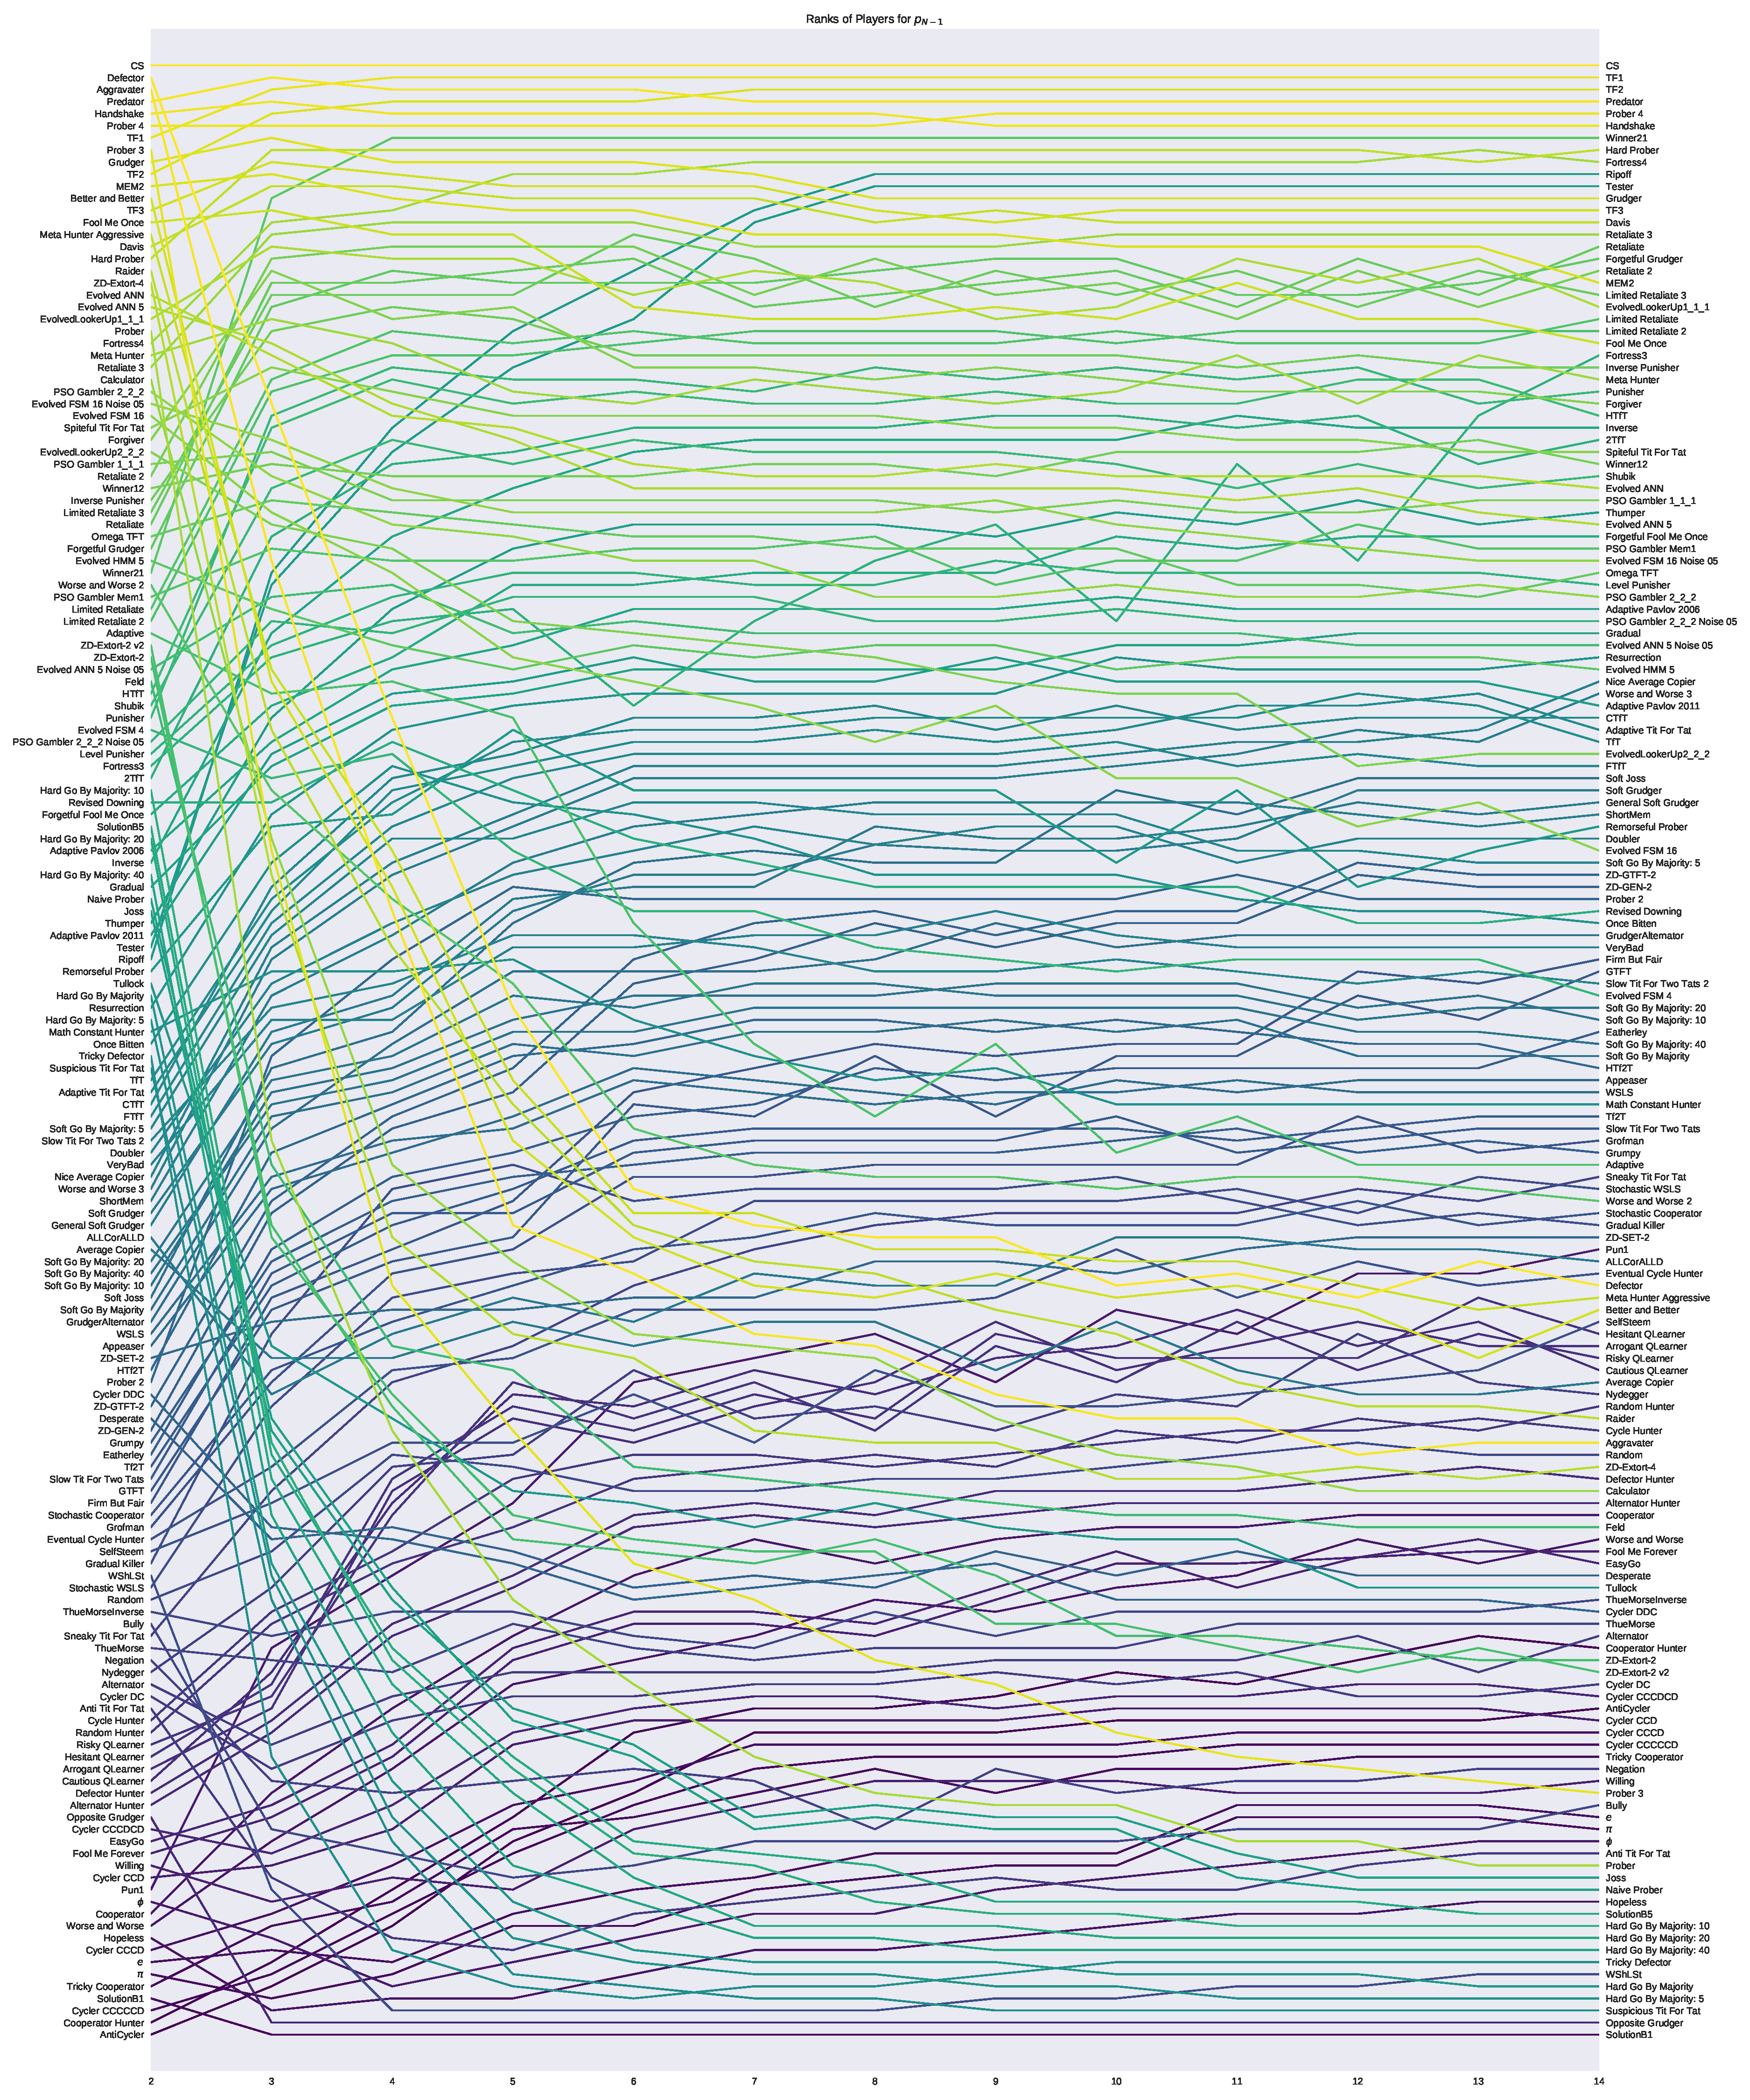
\includegraphics[height=.9\textheight]{./img/average_rank_vs_population_size_resist.pdf}
    \caption{Ranks of all strategies according to \(x_{N-1}\) for different
    population sizes}
    \label{fig:ranks_v_size_resist}
\end{figure}

\begin{table}[!hbtp]
    \centering
    \scriptsize
    \begin{tabular}{lrrrrrrrrrrr}
\toprule
        Player &     2 &      3 &      4 &      5 &      6 &      7 &      8 &      9 &     10 &     11 &     12 \\
\midrule
   ZD-Extort-4 &   1.0 &   10.0 &  103.0 &  108.0 &  118.0 &  120.5 &  123.5 &  122.0 &  124.5 &  129.0 &  128.5 \\
            CS &   2.0 &    1.0 &    1.0 &    1.0 &    1.0 &    2.0 &    2.0 &    2.0 &    2.0 &   48.5 &   49.5 \\
 Trained FSM 3 &   3.0 &  105.5 &  103.0 &  106.5 &  112.5 &  114.0 &  115.0 &  110.0 &  112.0 &  110.0 &  114.0 \\
          Feld &   4.5 &    6.0 &    6.0 &   99.5 &  103.0 &   99.0 &  108.0 &  107.0 &  103.0 &  109.0 &  113.0 \\
   ZD-Extort-2 &   4.5 &   13.5 &  112.0 &  113.5 &  119.5 &  123.0 &  125.0 &  126.5 &  134.0 &  130.0 &  142.5 \\
            CS &   3.0 &    1.0 &    1.0 &    1.0 &    1.0 &    1.0 &    1.0 &    1.0 &    1.0 &    1.0 &    1.0 \\
     Handshake &  17.0 &    3.0 &    3.0 &    3.0 &    3.0 &    3.0 &    3.0 &    2.0 &    3.0 &    3.0 &    2.5 \\
      Predator &   8.0 &    2.0 &    2.0 &    2.0 &    2.0 &    2.0 &    2.0 &    3.0 &    2.0 &    2.0 &    2.5 \\
      Prober 4 &  11.0 &    4.0 &    4.0 &    4.0 &    4.0 &    4.0 &    5.0 &    4.0 &    6.0 &    4.0 &    4.0 \\
      Winner21 &  22.0 &    5.0 &    5.0 &    5.0 &    5.0 &    5.0 &    4.0 &    5.0 &    4.0 &    5.0 &    5.0 \\
\bottomrule
\end{tabular}

    \caption{Ranks of some strategies according to \(x_{N-1}\) for different
    population sizes}
    \label{tbl:ranks_v_size_resist}
\end{table}

\begin{figure}[!hbtp]
    \centering
    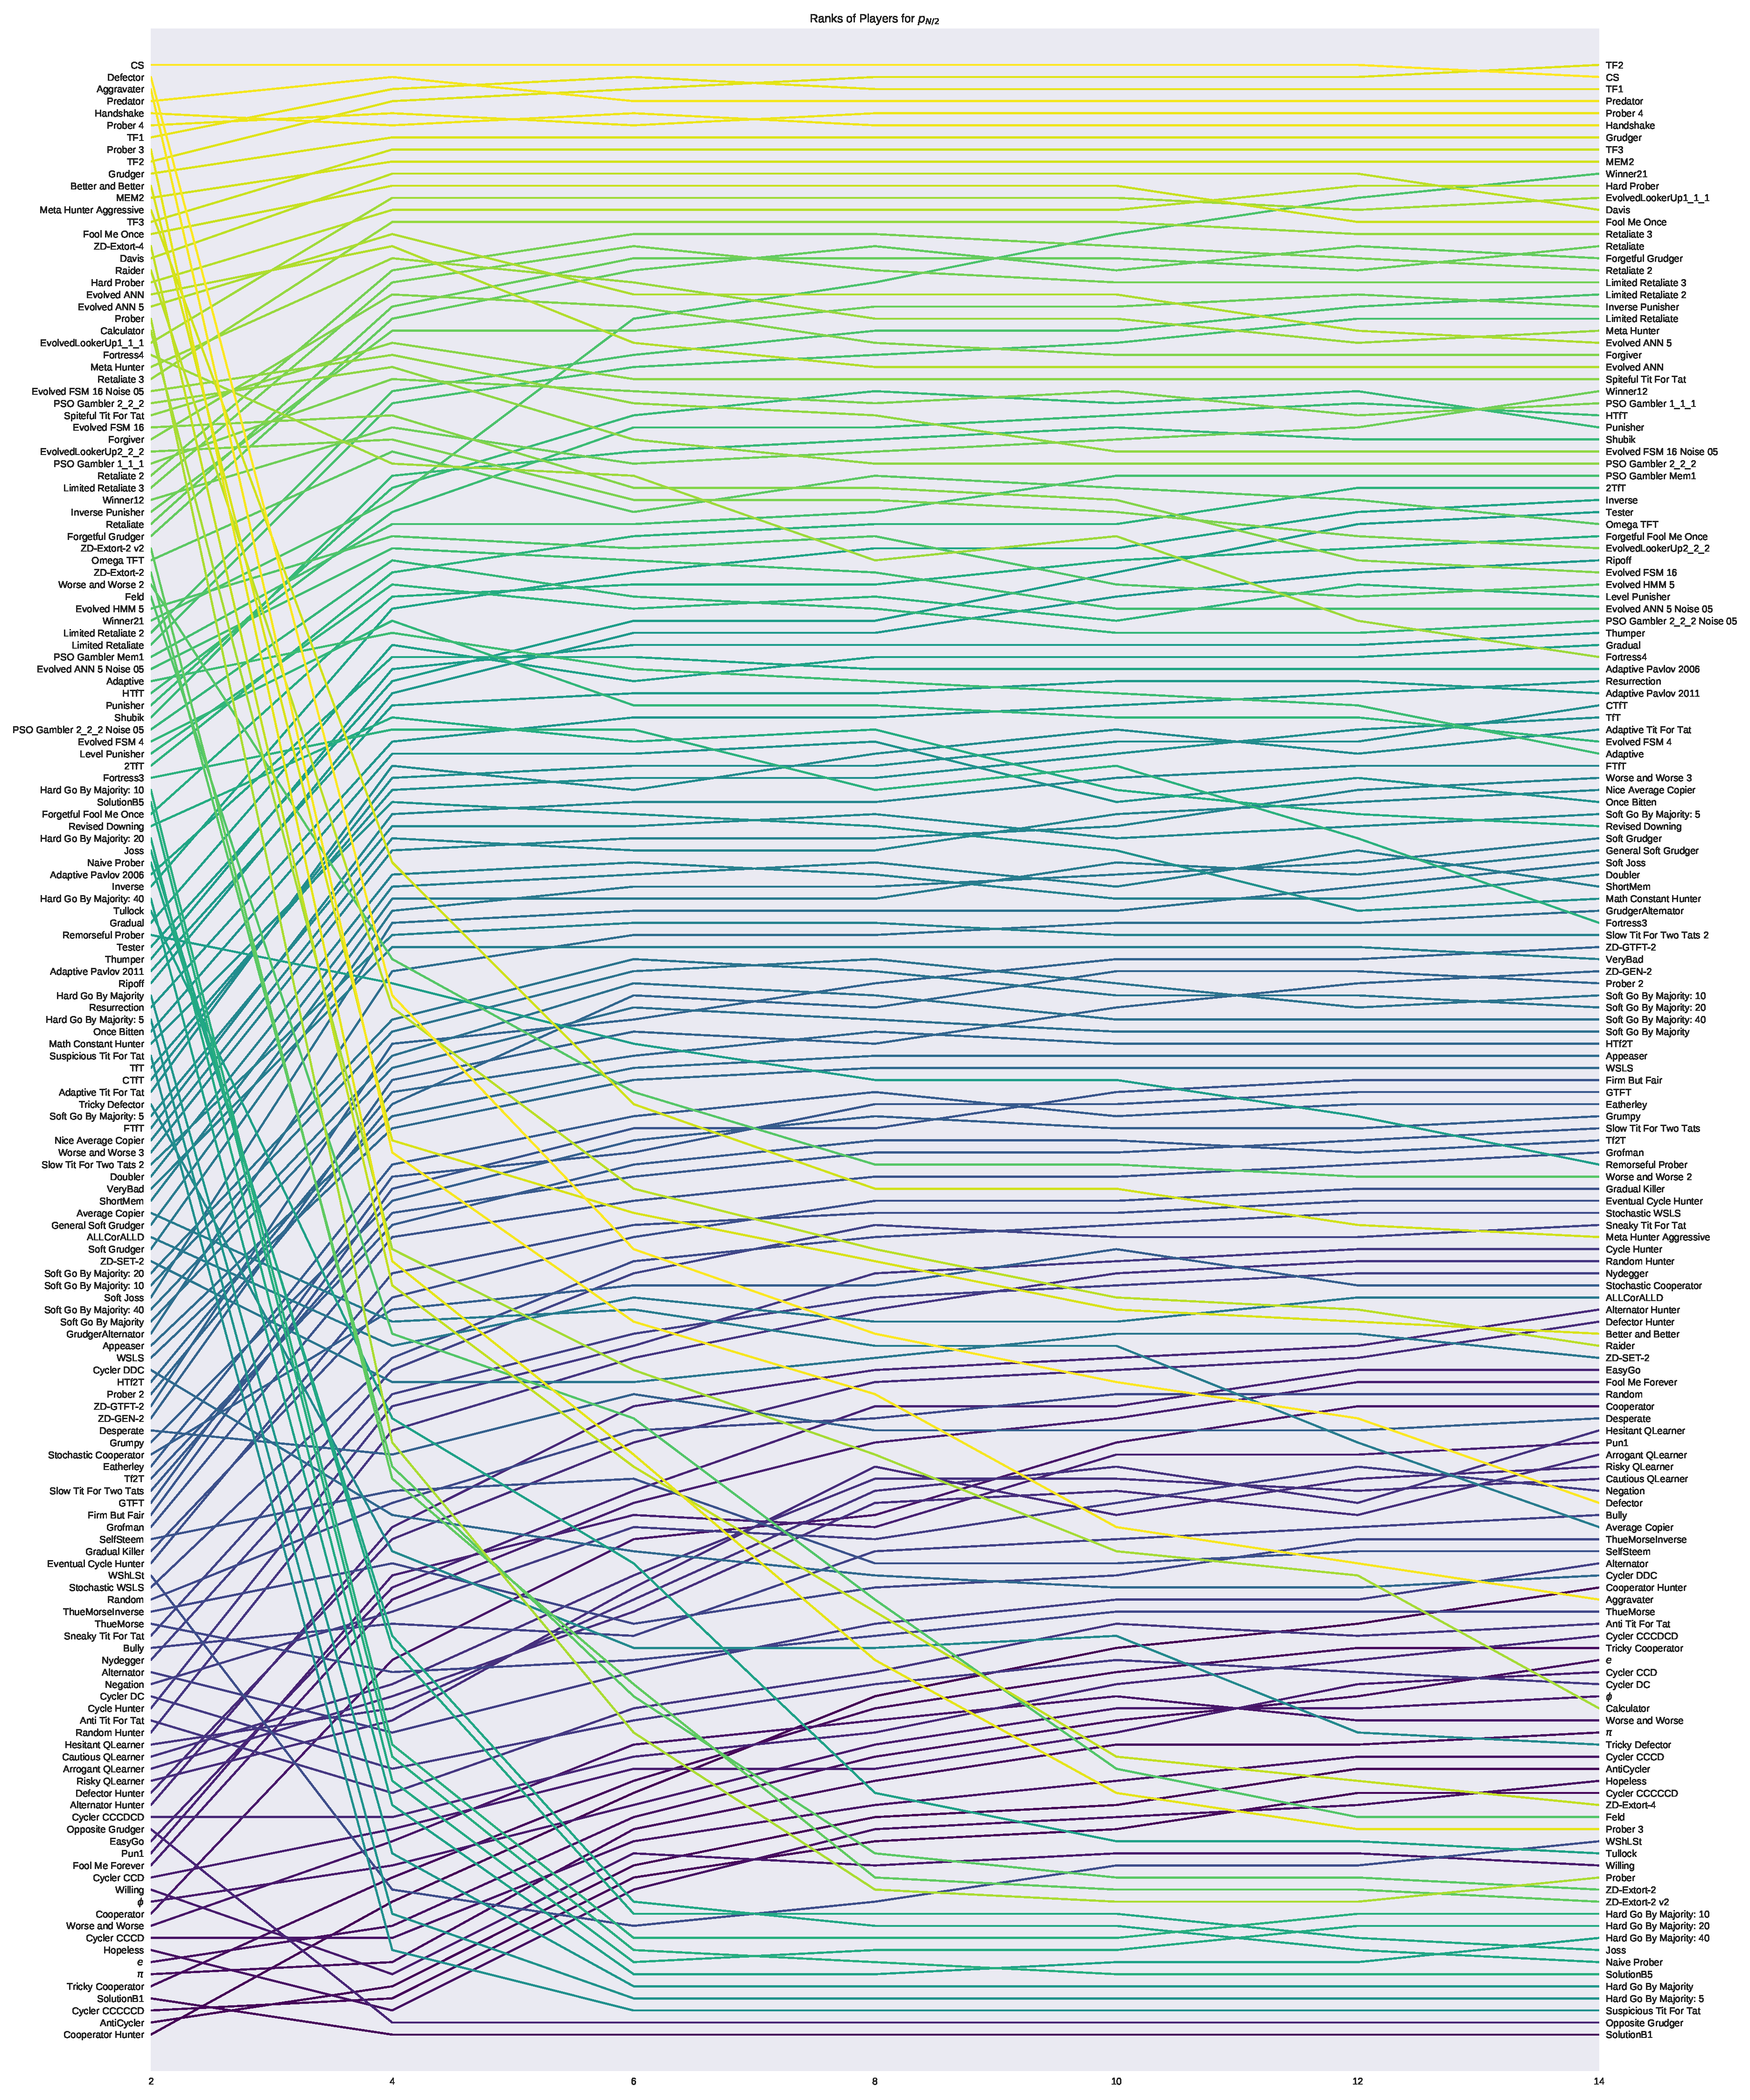
\includegraphics[height=.9\textheight]{./img/average_rank_vs_population_size_coexist.pdf}
    \caption{Ranks of all strategies according to \(x_{N/2}\) for different
    population sizes}
    \label{fig:ranks_v_size_coexist}
\end{figure}

\begin{table}[!hbtp]
    \centering
    \scriptsize
    \begin{tabular}{lrrrrrr}
\toprule
                                            Player &     2 &      4 &      6 &      8 &     10 &     12 \\
\midrule
         ZD-Extort-4: 0.23529411764705882, 0.25, 1 &   1.0 &  103.0 &  118.0 &  123.5 &  124.5 &  128.5 \\
                                CollectiveStrategy &   2.0 &    1.0 &    1.0 &    2.0 &    2.0 &   49.5 \\
 FSM Player: [(0, 'C', 7, 'C'), (0, 'D', 1, 'C'... &   3.0 &  103.0 &  112.5 &  115.0 &  112.0 &  114.0 \\
                               Feld: 1.0, 0.5, 200 &   4.5 &    6.0 &  103.0 &  108.0 &  103.0 &  113.0 \\
              ZD-Extort-2: 0.1111111111111111, 0.5 &   4.5 &  112.0 &  119.5 &  125.0 &  134.0 &  142.5 \\
                                CollectiveStrategy &   2.0 &    1.0 &    1.0 &    1.0 &    1.0 &    1.0 \\
                                          Predator &   9.0 &    2.0 &    2.0 &    2.0 &    2.0 &    2.0 \\
                                          Prober 4 &  11.0 &    3.0 &    3.0 &    3.0 &    3.0 &    3.0 \\
                                         Handshake &  14.5 &    4.0 &    4.0 &    4.0 &    4.0 &    4.0 \\
                                         Fortress4 &  29.0 &    8.5 &    8.0 &    7.0 &    5.0 &    5.0 \\
\bottomrule
\end{tabular}

    \caption{Ranks of some strategies according to \(x_{N/2}\) for different
    population sizes}
    \label{tbl:ranks_v_size_coexist}
\end{table}

% TODO Add discussion about ZD strategies

\begin{table}[!hbtp]
    \centering
    \scriptsize
    \begin{tabular}{lrrrrrrrrrrrrr}
\toprule
         player &      2 &      3 &      4 &      5 &      6 &      7 &      8 &      9 &     10 &     11 &     12 &     13 &     14 \\
\midrule
    ZD-Extort-4 &   16.0 &   81.0 &  107.0 &  120.0 &  135.0 &  136.0 &  142.0 &  140.0 &  142.0 &  142.0 &  144.0 &  144.0 &  145.0 \\
 ZD-Extort-2 v2 &   41.0 &  105.0 &  126.0 &  140.0 &  152.0 &  152.0 &  153.0 &  152.0 &  153.0 &  153.0 &  153.0 &  152.0 &  153.0 \\
    ZD-Extort-2 &   43.0 &  107.0 &  125.0 &  139.0 &  151.0 &  151.0 &  152.0 &  153.0 &  152.0 &  152.0 &  152.0 &  153.0 &  152.0 \\
       ZD-SET-2 &  100.0 &  111.0 &  117.0 &  117.0 &  122.0 &  127.0 &  131.0 &  128.0 &  131.0 &  131.0 &  130.0 &  132.0 &  131.0 \\
      ZD-GTFT-2 &  112.0 &   92.0 &   82.0 &   80.0 &   81.0 &   82.0 &   84.0 &   72.0 &   81.0 &   71.0 &   78.0 &   72.0 &   70.0 \\
       ZD-GEN-2 &  113.0 &   96.0 &   87.0 &   83.0 &   85.0 &   88.0 &   90.0 &   82.0 &   87.0 &   82.0 &   86.0 &   83.0 &   91.0 \\
\bottomrule
\end{tabular}

    \caption{Ranks of Zero determinant strategies according to \(x_{1}\) for different
    population sizes}
    \label{tbl:ZD_ranks_v_invade}
\end{table}

\begin{table}[!hbtp]
    \centering
    \scriptsize
    \begin{tabular}{lrrrrrrrrrrrrr}
\toprule
         player &      2 &      3 &      4 &      5 &      6 &      7 &      8 &      9 &     10 &     11 &     12 &     13 &     14 \\
\midrule
    ZD-Extort-4 &   19.0 &   68.0 &   98.0 &  106.0 &  108.0 &  114.0 &  115.0 &  115.0 &  118.0 &  118.0 &  117.0 &  118.0 &  117.0 \\
 ZD-Extort-2 v2 &   49.0 &   98.0 &  111.0 &  121.0 &  123.0 &  124.0 &  124.0 &  130.0 &  130.0 &  132.0 &  134.0 &  132.0 &  134.0 \\
    ZD-Extort-2 &   50.0 &   97.0 &  112.0 &  123.0 &  124.0 &  125.0 &  123.0 &  126.0 &  131.0 &  131.0 &  132.0 &  133.0 &  133.0 \\
       ZD-SET-2 &  108.0 &  105.0 &  104.0 &  104.0 &  103.0 &  103.0 &  100.0 &  100.0 &  101.0 &   99.0 &   98.0 &   98.0 &   98.0 \\
        ZD-GTFT &  112.0 &   95.0 &   88.0 &   84.0 &   75.0 &   72.0 &   71.0 &   73.0 &   71.0 &   71.0 &   67.0 &   68.0 &   68.0 \\
       ZD-GEN-2 &  114.0 &   96.0 &   89.0 &   86.0 &   77.0 &   75.0 &   72.0 &   74.0 &   72.0 &   72.0 &   68.0 &   69.0 &   69.0 \\
\bottomrule
\end{tabular}

    \caption{Ranks of Zero determinant strategies according to \(x_{N-1}\) for different
    population sizes}
    \label{tbl:ZD_ranks_v_size_resist}
\end{table}

\begin{table}[!hbtp]
    \centering
    \scriptsize
    \begin{tabular}{lrrrrrrr}
\toprule
         player &      2 &      4 &      6 &      8 &     10 &     12 &     14 \\
\midrule
    ZD-Extort-4 &   16.0 &  102.0 &  117.0 &  129.0 &  141.0 &  143.0 &  145.0 \\
 ZD-Extort-2 v2 &   41.0 &  118.0 &  135.0 &  151.0 &  152.0 &  152.0 &  153.0 \\
    ZD-Extort-2 &   43.0 &  117.0 &  136.0 &  149.0 &  151.0 &  151.0 &  152.0 \\
       ZD-SET-2 &  100.0 &  110.0 &  110.0 &  108.0 &  106.0 &  106.0 &  108.0 \\
      ZD-GTFT-2 &  112.0 &   82.0 &   80.0 &   77.0 &   75.0 &   75.0 &   74.0 \\
       ZD-GEN-2 &  113.0 &   85.0 &   81.0 &   82.0 &   79.0 &   77.0 &   76.0 \\
\bottomrule
\end{tabular}

    \caption{Ranks of Zero determinant strategies according to \(x_{N/2}\) for different
    population sizes}
    \label{tbl:ZD_ranks_v_size_coexist}
\end{table}

Tables~\ref{tbl:correlation_coeficients_invade},~\ref{tbl:correlation_coeficients_resist}
and~\ref{tbl:correlation_coeficients_coexist} show the correlation coefficients
of the ranks of strategies in differing population size. This is shown
graphically in Figure~\ref{fig:correlation_coefficients}. It is immediate to
note that how well a strategy performs in any Moran process for \(N>2\) has
little to do with the performance for \(N=2\). This illustrates why the strong
performance of zero determinant strategies predicted in \cite{Press2012} does
not extend to larger populations. This was discussed theoretically in
\cite{Adami2013} however not observed empirically at the scale presented here.

\begin{table}[!hbtp]
    \centering
    \begin{subfigure}{\textwidth}
        \centering
        \begin{tabular}{lrrrrrrrrr}
\toprule
N &    2  &    3  &    4  &    5  &    6  &    7  &    8  &    9  &    10 \\
\midrule
2  &  1.00 &  0.44 &  0.26 &  0.17 &  0.15 &  0.12 &  0.08 &  0.07 &  0.08 \\
3  &  0.44 &  1.00 &  0.92 &  0.87 &  0.87 &  0.86 &  0.83 &  0.83 &  0.84 \\
4  &  0.26 &  0.92 &  1.00 &  0.97 &  0.96 &  0.97 &  0.95 &  0.95 &  0.95 \\
5  &  0.17 &  0.87 &  0.97 &  1.00 &  0.98 &  0.99 &  0.97 &  0.98 &  0.98 \\
6  &  0.15 &  0.87 &  0.96 &  0.98 &  1.00 &  0.99 &  0.97 &  0.97 &  0.98 \\
7  &  0.12 &  0.86 &  0.97 &  0.99 &  0.99 &  1.00 &  0.98 &  0.98 &  0.99 \\
8  &  0.08 &  0.83 &  0.95 &  0.97 &  0.97 &  0.98 &  1.00 &  0.97 &  0.98 \\
9  &  0.07 &  0.83 &  0.95 &  0.98 &  0.97 &  0.98 &  0.97 &  1.00 &  0.99 \\
10 &  0.08 &  0.84 &  0.95 &  0.98 &  0.98 &  0.99 &  0.98 &  0.99 &  1.00 \\
\bottomrule
\end{tabular}

        \caption{Correlation coefficients for ranks for invasion}
        \label{tbl:correlation_coeficients_invade}
    \end{subfigure}%

    \begin{subfigure}{\textwidth}
        \centering
        \begin{tabular}{lrrrrrrrrrr}
\toprule
N &    2  &    3  &    4  &    5  &    6  &    7  &    8  &    9  &    10 &    12 \\
\midrule
2  &  1.00 &  0.61 &  0.42 &  0.29 &  0.35 &  0.34 &  0.34 &  0.20 &  0.30 &  0.27 \\
3  &  0.61 &  1.00 &  0.91 &  0.81 &  0.87 &  0.87 &  0.87 &  0.76 &  0.85 &  0.83 \\
4  &  0.42 &  0.91 &  1.00 &  0.93 &  0.98 &  0.97 &  0.97 &  0.89 &  0.96 &  0.95 \\
5  &  0.29 &  0.81 &  0.93 &  1.00 &  0.93 &  0.94 &  0.94 &  0.96 &  0.93 &  0.92 \\
6  &  0.35 &  0.87 &  0.98 &  0.93 &  1.00 &  0.98 &  0.98 &  0.92 &  0.99 &  0.99 \\
7  &  0.34 &  0.87 &  0.97 &  0.94 &  0.98 &  1.00 &  1.00 &  0.92 &  0.99 &  0.98 \\
8  &  0.34 &  0.87 &  0.97 &  0.94 &  0.98 &  1.00 &  1.00 &  0.91 &  0.98 &  0.98 \\
9  &  0.20 &  0.76 &  0.89 &  0.96 &  0.92 &  0.92 &  0.91 &  1.00 &  0.93 &  0.93 \\
10 &  0.30 &  0.85 &  0.96 &  0.93 &  0.99 &  0.99 &  0.98 &  0.93 &  1.00 &  1.00 \\
12 &  0.27 &  0.83 &  0.95 &  0.92 &  0.99 &  0.98 &  0.98 &  0.93 &  1.00 &  1.00 \\
\bottomrule
\end{tabular}

        \caption{Correlation coefficients for ranks for resistance}
        \label{tbl:correlation_coeficients_resist}
    \end{subfigure}

    \begin{subfigure}{\textwidth}
        \centering
        \begin{tabular}{lrrrrrr}
\toprule
N &    2  &    4  &    6  &    8  &    10 &    12 \\
\midrule
2  &  1.00 &  0.25 &  0.19 &  0.12 &  0.13 &  0.09 \\
4  &  0.25 &  1.00 &  0.99 &  0.97 &  0.98 &  0.97 \\
6  &  0.19 &  0.99 &  1.00 &  0.98 &  1.00 &  0.98 \\
8  &  0.12 &  0.97 &  0.98 &  1.00 &  0.99 &  1.00 \\
10 &  0.13 &  0.98 &  1.00 &  0.99 &  1.00 &  0.99 \\
12 &  0.09 &  0.97 &  0.98 &  1.00 &  0.99 &  1.00 \\
\bottomrule
\end{tabular}

        \caption{Correlation coefficients for ranks for coexistance}
        \label{tbl:correlation_coeficients_coexist}
    \end{subfigure}
    \caption{Correlation coefficients of rankings by population size}
\end{table}

\begin{figure}[!htbp]
    \centering
    \begin{subfigure}[t]{.3\textwidth}
        \centering
        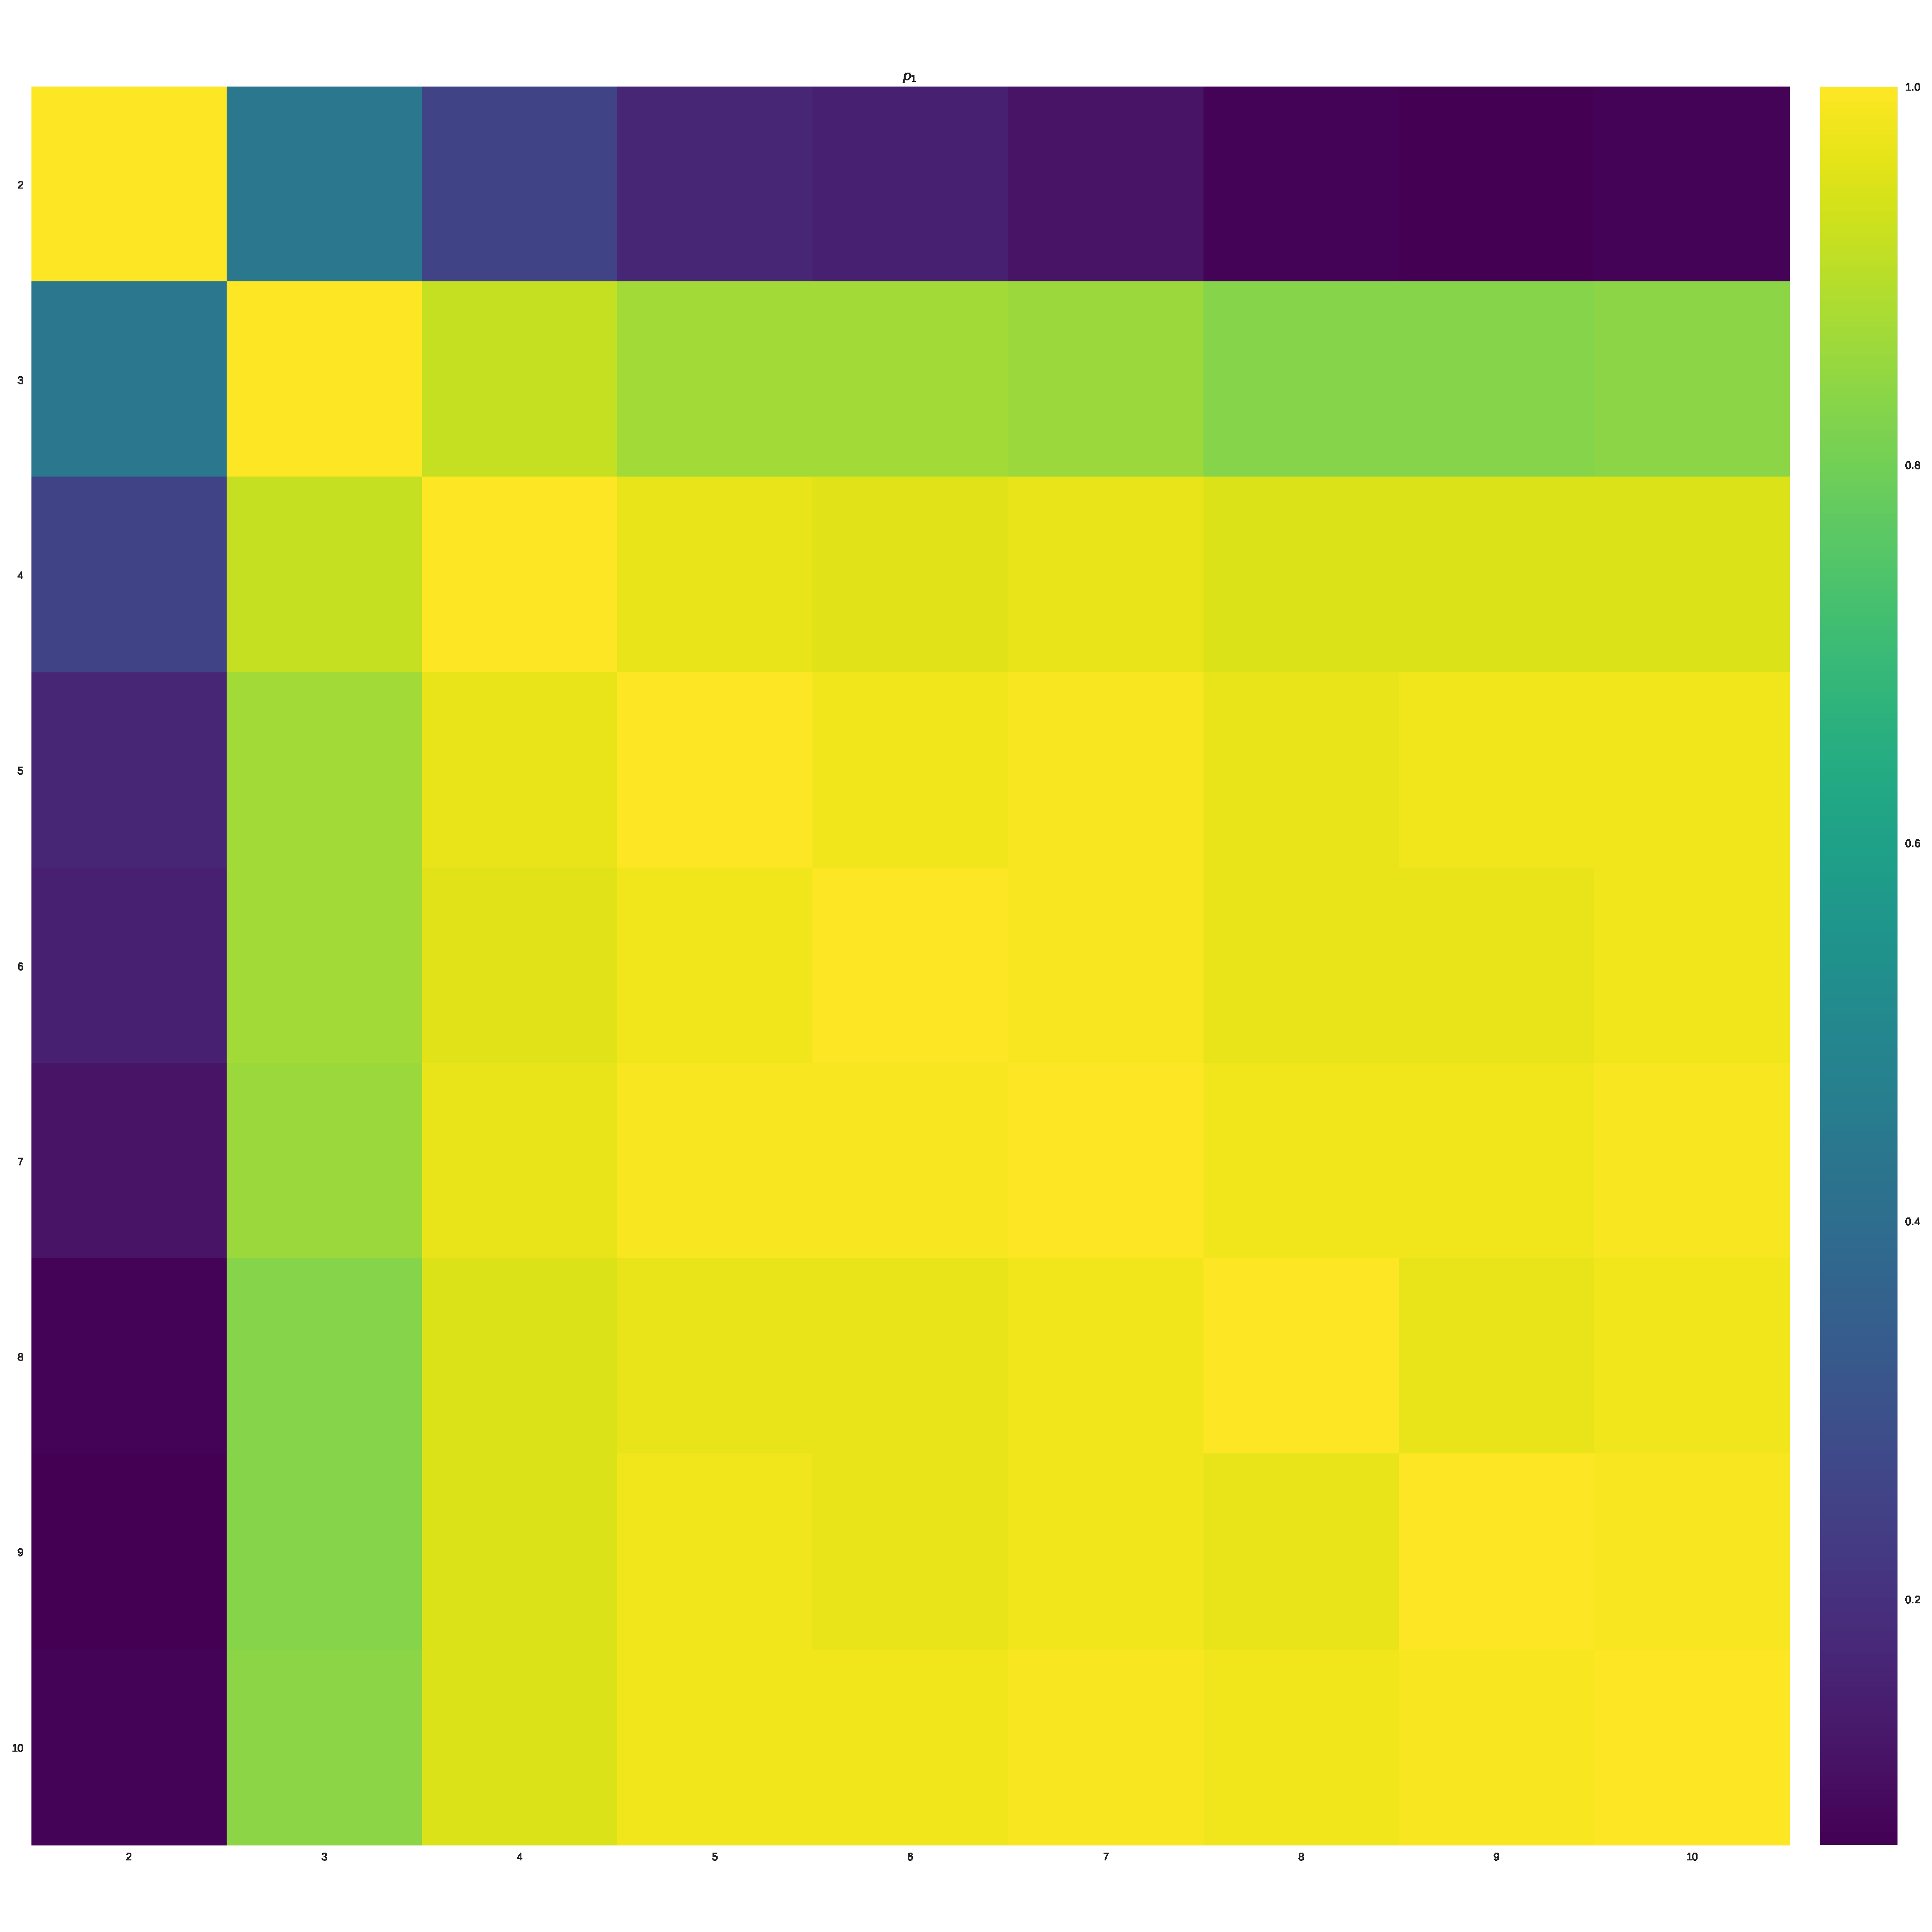
\includegraphics[width=.9\textwidth]{./img/correlation_heatmap_invade.pdf}
        \caption{Rank based on \(x_1\)}
    \end{subfigure}
    ~
    \begin{subfigure}[t]{.3\textwidth}
        \centering
        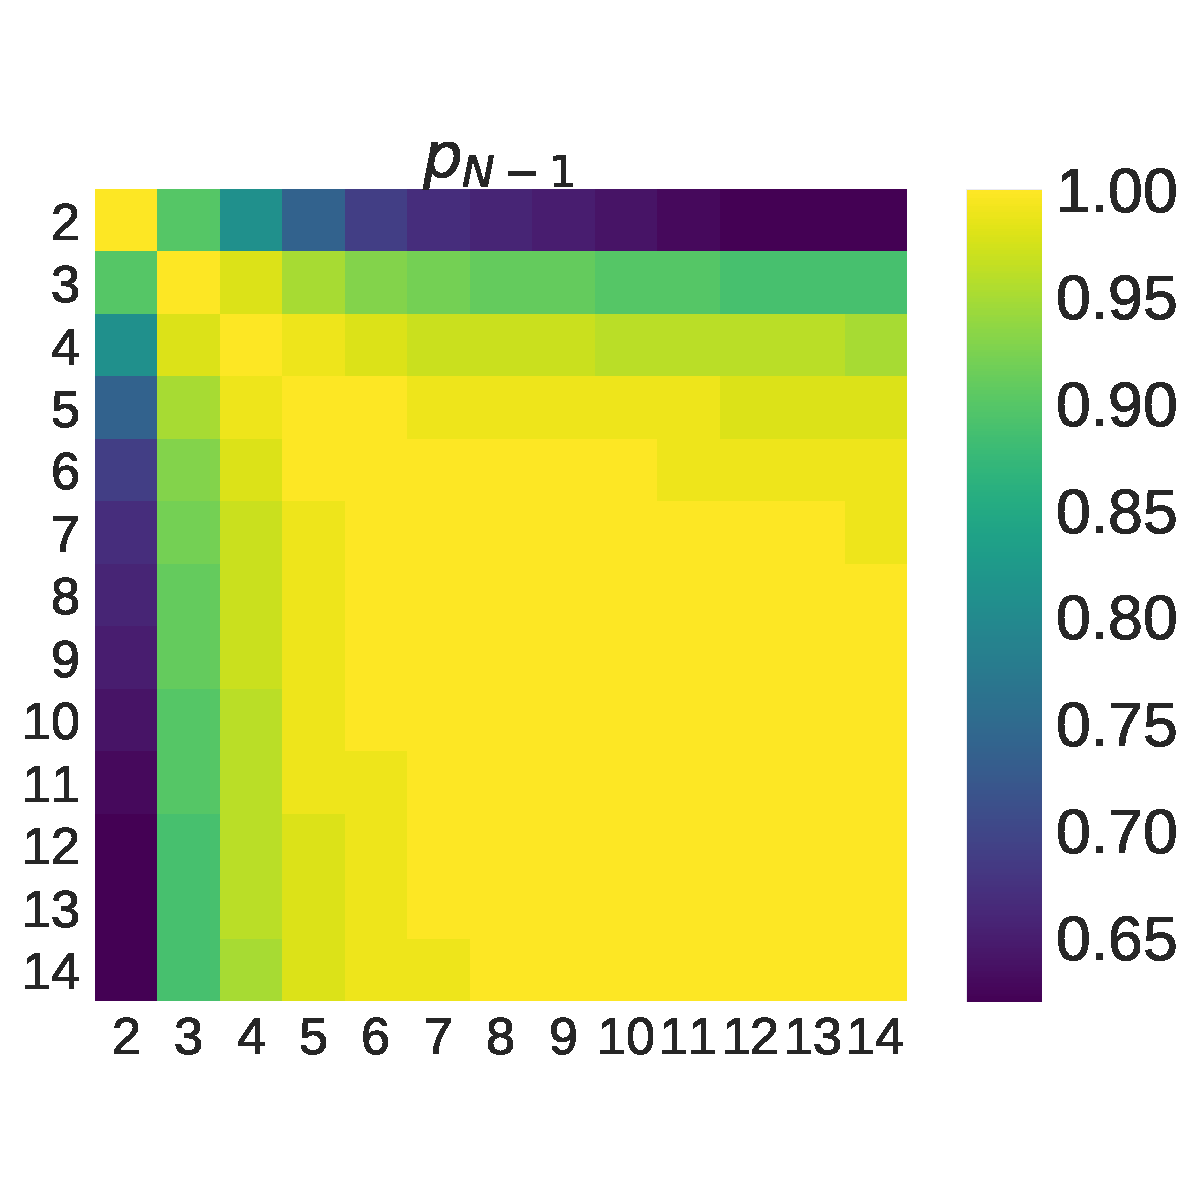
\includegraphics[width=.9\textwidth]{./img/correlation_heatmap_resist.pdf}
        \caption{Rank based on \(x_{N - 1}\)}
    \end{subfigure}
    ~
    \begin{subfigure}[t]{.3\textwidth}
        \centering
        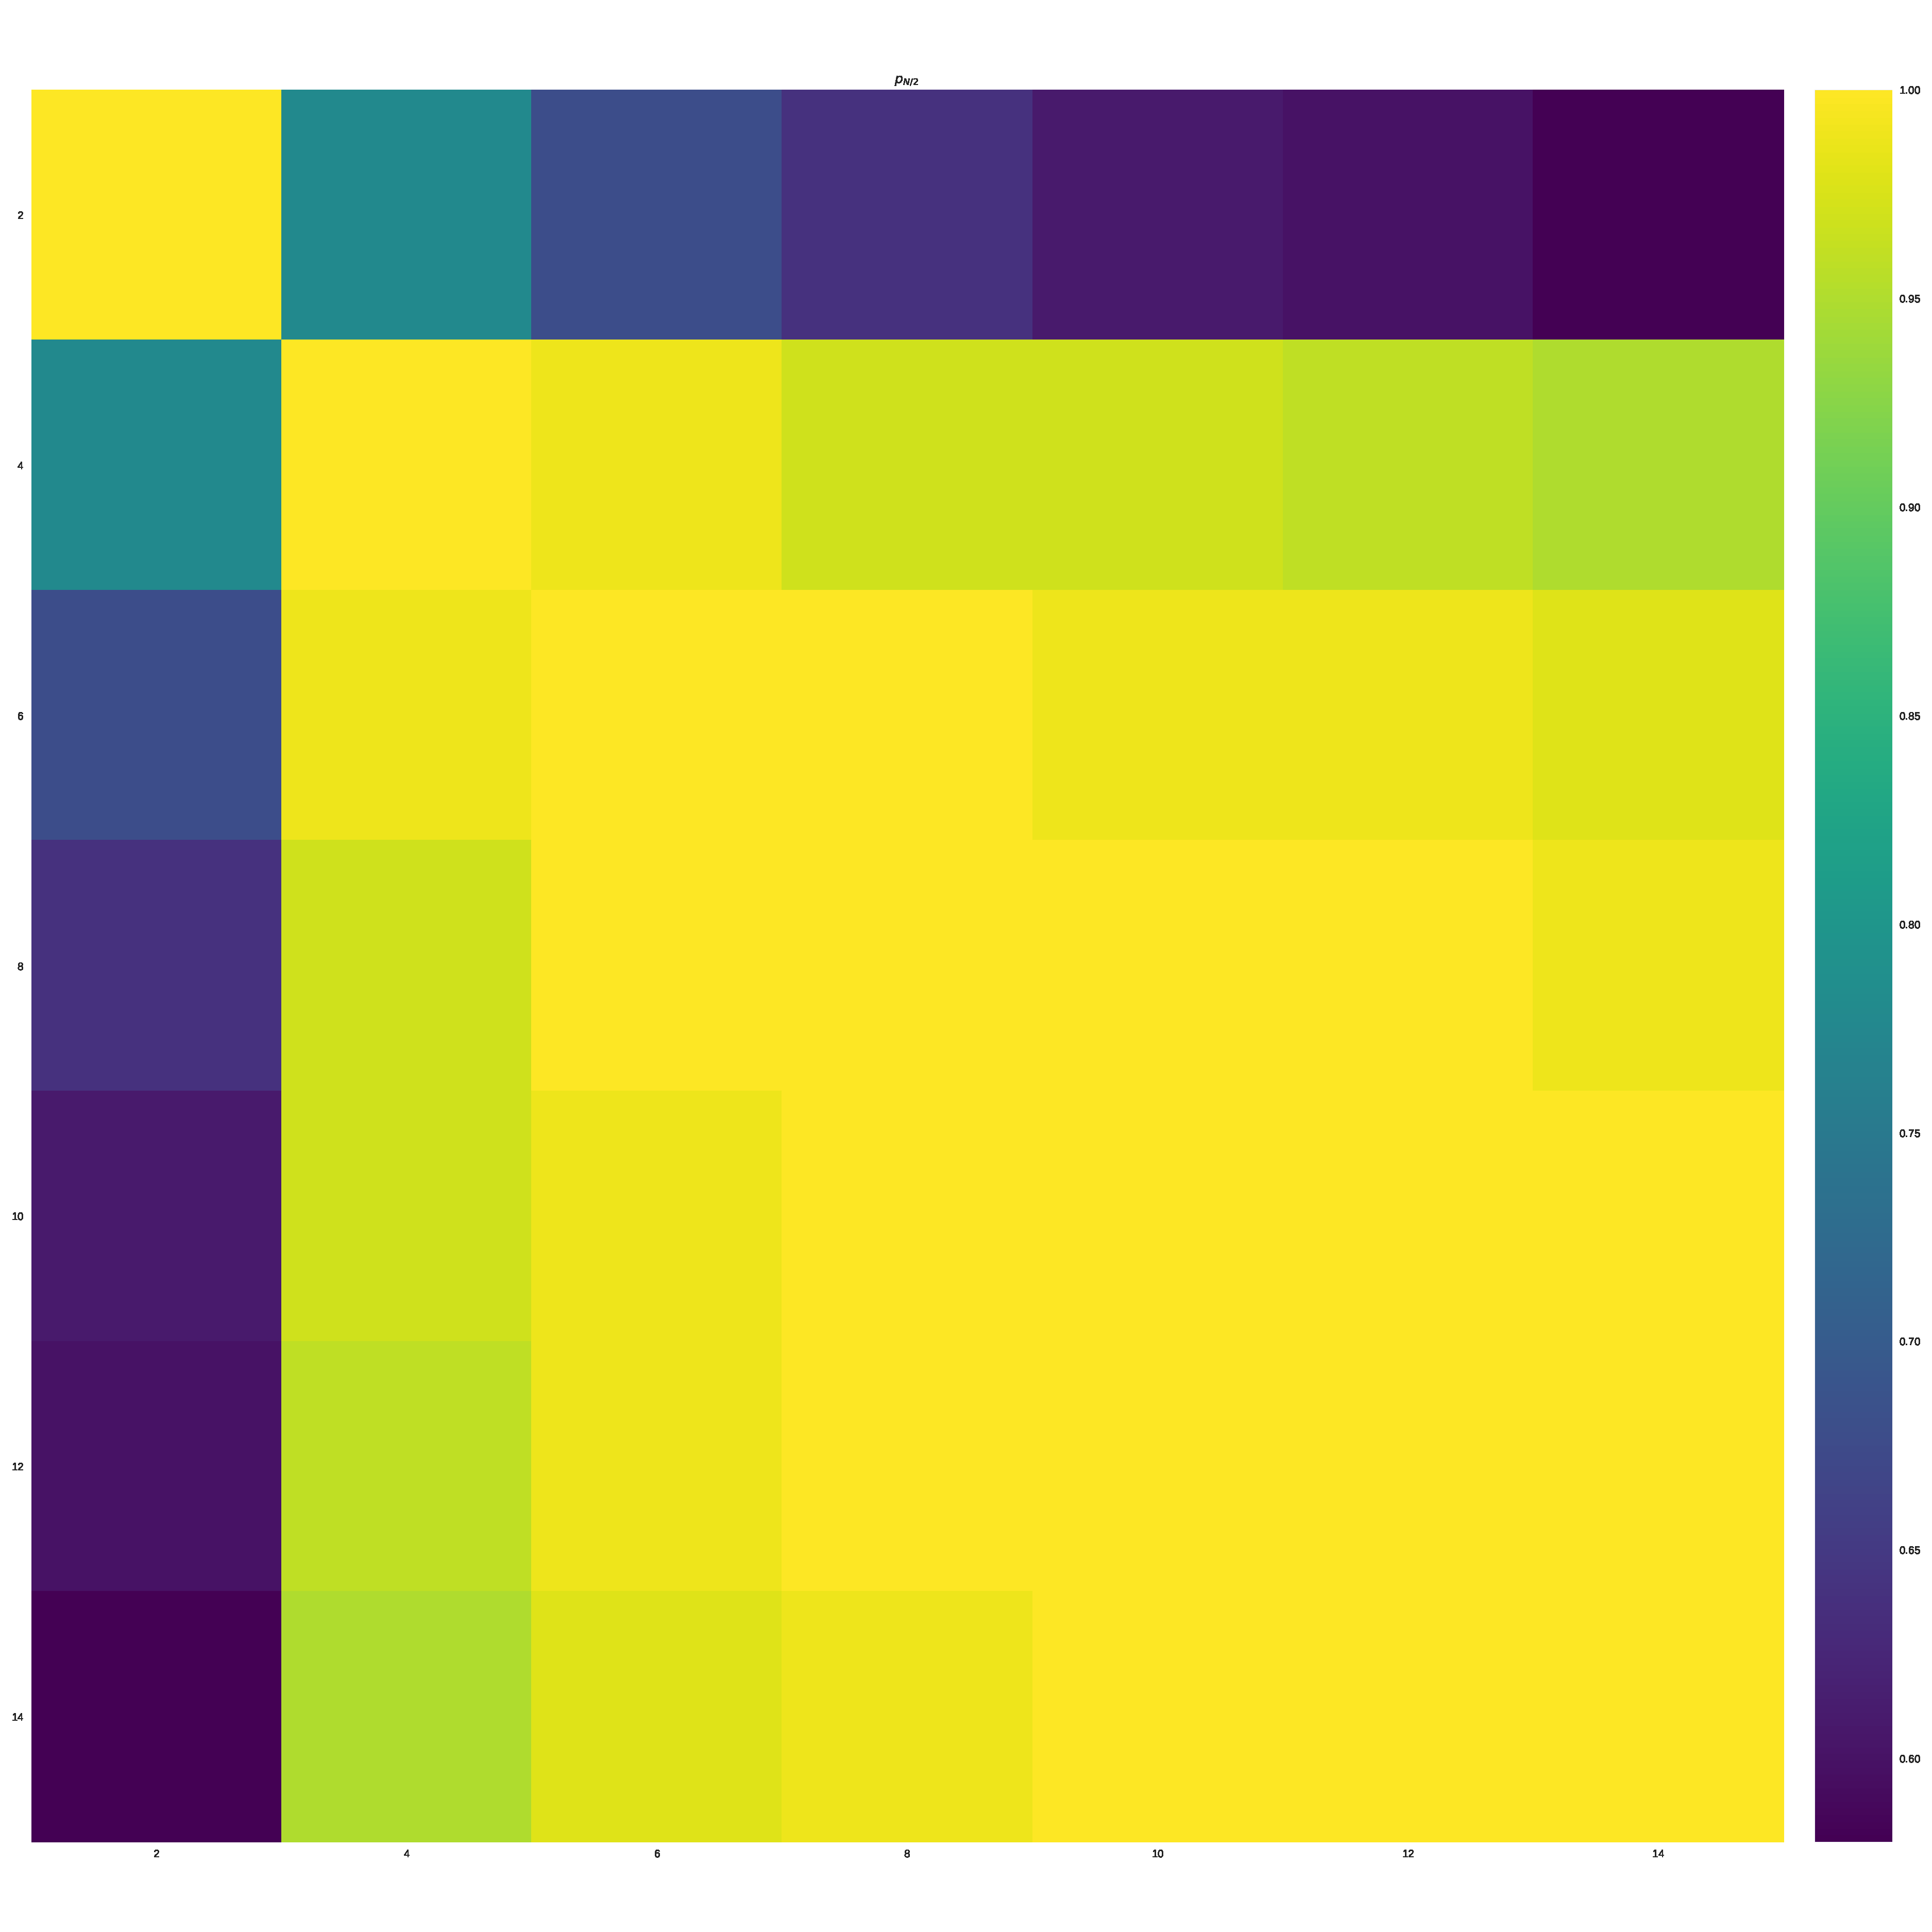
\includegraphics[width=.9\textwidth]{./img/correlation_heatmap_coexist.pdf}
        \caption{Rank based on \(x_{N/2}\)}
    \end{subfigure}
    \caption{Heatmap of correlation coefficients of rankings by population size}
    \label{fig:correlation_coefficients}
\end{figure}


\section{Conclusion}\label{sec:conclusion}

A detailed empirical analysis of 164 strategies of the IPD within a pairwise
Moran process has been carried out. All \(\binom{164}{2}=13,366\) possible
ordered pairs of strategies have been placed in a Moran process with different
starting values allowing the each strategy to attempt to invade the other.

This is the largest such experiment carried out and has lead to many insights.

When studying evolutionary processes it is vital to consider \(N>2\) as the
special case for \(N=2\) cannot be used to extrapolate performance in bigger
populations. This was shown both observationally in
Sections~\ref{sec:strong_invaders} and~\ref{sec:strong_resistors} but also by
considering the correlation of the ranks in different population sizes in
Section~\ref{sec:population_size}.

Memory one strategies do not perform well, as predicted by \cite{Press2012}.
However, there are no memory one strategies in the top 5 performing strategies
for \(N>3\). This is due to their lack of sophistication which allows them to
recognise and adjust to their opponent. Some very sophisticated strategies
proves to be high performers for invasion: these are infinite memory strategies
which have been trained using a number of reinforcement learning algorithms.
Interestingly they have been trained to perform well in tournaments and not
Moran processes which highlights the potentially for improvement.

It is felt that these findings are important for the ongoing understanding of
population dynamics and offer evidence for some of the shortcomings of short
memory which has started to be recognised by the community~\cite{Hilbe2017}.

All source code for this work has been written in a sustainable manner: it is
open source, under version control and tested which ensures that all results can
be reproduced \cite{Prlic2012, Sandve2013, Wilson2014}. The raw data as well as
the processed data has also been properly archived.

There are various areas for further work to build on this. Firstly, an analysis
of the effect of noise would offer insights about the stability of the findings.
It would also be possible to consider three or more types of strategy in the
population and finally mutation would also offer an interesting dimension to
explore.

\section*{Acknowledgements}

This work was performed using the computational facilities of the Advanced
Research Computing @ Cardiff (ARCCA) Division, Cardiff University.

A variety of software libraries have been used in this work:

\begin{itemize}
    \item The Axelrod library (IPD strategies and Moran processes)
        \cite{axelrodproject}.
    \item The matplotlib library (visualisation) \cite{hunter2007matplotlib}.
    \item The pandas and numpy libraries (data manipulation)
        \cite{mckinney2010data, walt2011numpy}.
\end{itemize}

\printbibliography

\appendix

\section{List of players}\label{app:list_of_players}

\begin{multicols}{3}
	\begin{enumerate}
		\item $\phi$
\item $\pi$
\item $e$
\item ALLCorALLD
\item Adaptive
\item Adaptive Pavlov 2006
\item Adaptive Pavlov 2011
\item Adaptive Tit For Tat: 0.5
\item Aggravater
\item Alternator
\item Alternator Hunter
\item Anti Tit For Tat
\item AntiCycler
\item Appeaser
\item Arrogant QLearner
\item Average Copier
\item Better and Better
\item Bully
\item Calculator
\item Cautious QLearner
\item CollectiveStrategy
(\textbf{CS})\item Contrite Tit For Tat
\item Cooperator
\item Cooperator Hunter
\item Cycle Hunter
\item Cycler CCCCCD
\item Cycler CCCD
\item Cycler CCCDCD
\item Cycler CCD
\item Cycler DC
\item Cycler DDC
\item Davis: 10
\item Defector
\item Defector Hunter
\item Desperate
\item Doubler
\item EasyGo
\item Eatherley
\item Eventual Cycle Hunter
\item Evolved ANN
\item Evolved ANN 5
\item Evolved ANN 5 Noise 05
\item Evolved FSM 16
\item Evolved FSM 16 Noise 05
\item Evolved FSM 4
\item Evolved HMM 5
\item EvolvedLookerUp1\_1\_1
\item EvolvedLookerUp2\_2\_2
\item FSM Player: [(0, 'C', 0, 'C'), (0, 'D', 3, 'C'), (1, 'C', 5, 'D'), (1, 'D', 0, 'C'), (2, 'C', 3, 'C'), (2, 'D', 2, 'D'), (3, 'C', 4, 'D'), (3, 'D', 6, 'D'), (4, 'C', 3, 'C'), (4, 'D', 1, 'D'), (5, 'C', 6, 'C'), (5, 'D', 3, 'D'), (6, 'C', 6, 'D'), (6, 'D', 6, 'D'), (7, 'C', 7, 'D'), (7, 'D', 5, 'C')], 1, C
(\textbf{Trained FSM 1})\item FSM Player: [(0, 'C', 13, 'D'), (0, 'D', 12, 'D'), (1, 'C', 3, 'D'), (1, 'D', 4, 'D'), (2, 'C', 14, 'D'), (2, 'D', 9, 'D'), (3, 'C', 0, 'C'), (3, 'D', 1, 'D'), (4, 'C', 1, 'D'), (4, 'D', 2, 'D'), (5, 'C', 12, 'C'), (5, 'D', 6, 'C'), (6, 'C', 1, 'C'), (6, 'D', 14, 'D'), (7, 'C', 12, 'D'), (7, 'D', 2, 'D'), (8, 'C', 7, 'D'), (8, 'D', 9, 'D'), (9, 'C', 8, 'D'), (9, 'D', 0, 'D'), (10, 'C', 2, 'C'), (10, 'D', 15, 'C'), (11, 'C', 7, 'D'), (11, 'D', 13, 'D'), (12, 'C', 3, 'C'), (12, 'D', 8, 'D'), (13, 'C', 7, 'C'), (13, 'D', 10, 'D'), (14, 'C', 10, 'D'), (14, 'D', 7, 'D'), (15, 'C', 15, 'C'), (15, 'D', 11, 'D')], 1, C
(\textbf{Trained FSM 2})\item FSM Player: [(0, 'C', 7, 'C'), (0, 'D', 1, 'C'), (1, 'C', 11, 'D'), (1, 'D', 11, 'D'), (2, 'C', 8, 'D'), (2, 'D', 8, 'C'), (3, 'C', 3, 'C'), (3, 'D', 12, 'D'), (4, 'C', 6, 'C'), (4, 'D', 3, 'C'), (5, 'C', 11, 'C'), (5, 'D', 8, 'D'), (6, 'C', 13, 'D'), (6, 'D', 14, 'C'), (7, 'C', 4, 'D'), (7, 'D', 2, 'D'), (8, 'C', 14, 'D'), (8, 'D', 8, 'D'), (9, 'C', 0, 'C'), (9, 'D', 10, 'D'), (10, 'C', 8, 'C'), (10, 'D', 15, 'C'), (11, 'C', 6, 'D'), (11, 'D', 5, 'D'), (12, 'C', 6, 'D'), (12, 'D', 9, 'D'), (13, 'C', 9, 'D'), (13, 'D', 8, 'D'), (14, 'C', 8, 'D'), (14, 'D', 13, 'D'), (15, 'C', 4, 'C'), (15, 'D', 5, 'C')], 1, C
(\textbf{Trained FSM 3})\item Feld: 1.0, 0.5, 200
\item Firm But Fair
\item Fool Me Forever
\item Fool Me Once
\item Forgetful Fool Me Once: 0.05
\item Forgetful Grudger
\item Forgiver
\item Forgiving Tit For Tat
\item Fortress3
\item Fortress4
\item GTFT: 0.33
\item General Soft Grudger: n=1,d=4,c=2
\item Gradual
\item Gradual Killer: ('D', 'D', 'D', 'D', 'D', 'C', 'C')
\item Grofman
\item Grudger
\item GrudgerAlternator
\item Grumpy: Nice, 10, -10
\item Handshake
\item Hard Go By Majority
\item Hard Go By Majority: 10
\item Hard Go By Majority: 20
\item Hard Go By Majority: 40
\item Hard Go By Majority: 5
\item Hard Prober
\item Hard Tit For 2 Tats
\item Hard Tit For Tat
\item Hesitant QLearner
\item Hopeless
\item Inverse
\item Inverse Punisher
\item Joss: 0.9
\item Level Punisher
\item Limited Retaliate 2: 0.08, 15
\item Limited Retaliate 3: 0.05, 20
\item Limited Retaliate: 0.1, 20
\item MEM2
\item Math Constant Hunter
\item Meta Hunter Aggressive: 7 players
\item Meta Hunter: 6 players
\item Naive Prober: 0.1
\item Negation
\item Nice Average Copier
\item Nydegger
\item Omega TFT: 3, 8
\item Once Bitten
\item Opposite Grudger
\item PSO Gambler 1\_1\_1
\item PSO Gambler 2\_2\_2
\item PSO Gambler 2\_2\_2 Noise 05
\item PSO Gambler Mem1
\item Predator
\item Prober
\item Prober 2
\item Prober 3
\item Prober 4
\item Pun1
\item Punisher
\item Raider
\item Random Hunter
\item Random: 0.5
\item Remorseful Prober: 0.1
\item Resurrection
\item Retaliate 2: 0.08
\item Retaliate 3: 0.05
\item Retaliate: 0.1
\item Revised Downing: True
\item Ripoff
\item Risky QLearner
\item SelfSteem
\item ShortMem
\item Shubik
\item Slow Tit For Two Tats
\item Slow Tit For Two Tats 2
\item Sneaky Tit For Tat
\item Soft Go By Majority
\item Soft Go By Majority: 10
\item Soft Go By Majority: 20
\item Soft Go By Majority: 40
\item Soft Go By Majority: 5
\item Soft Grudger
\item Soft Joss: 0.9
\item SolutionB1
\item SolutionB5
\item Spiteful Tit For Tat
\item Stochastic Cooperator
\item Stochastic WSLS: 0.05
\item Suspicious Tit For Tat
\item Tester
\item ThueMorse
\item ThueMorseInverse
\item Thumper
\item Tit For 2 Tats
(\textbf{Tf2T})\item Tit For Tat
(\textbf{TfT})\item Tricky Cooperator
\item Tricky Defector
\item Tullock: 11
\item Two Tits For Tat
(\textbf{2TfT})\item VeryBad
\item Willing
\item Win-Shift Lose-Stay: D
\item Win-Stay Lose-Shift: C
(\textbf{WSLS})\item Winner12
\item Winner21
\item Worse and Worse
\item Worse and Worse 2
\item Worse and Worse 3
\item ZD-Extort-2 v2: 0.125, 0.5, 1
\item ZD-Extort-2: 0.1111111111111111, 0.5
\item ZD-Extort-4: 0.23529411764705882, 0.25, 1
\item ZD-GEN-2: 0.125, 0.5, 3
\item ZD-GTFT-2: 0.25, 0.5
\item ZD-SET-2: 0.25, 0.0, 2

	\end{enumerate}
\end{multicols}

\end{document}
